\documentclass[12pt]{cs}

% =============================================================================
% Effective Context Length — Main Entry Point
% =============================================================================

% Packages
\usepackage{amsmath, amsfonts, amssymb}
\usepackage{amsthm}
\usepackage{mathtools}
\usepackage[ruled,vlined,linesnumbered]{algorithm2e}
\usepackage{float}
\usepackage{longtable}
\usepackage{array}
\usepackage{enumitem}
\usepackage{tabularx}
\usepackage{makecell}

% Algorithm2e cosmetics
\SetKwComment{Comment}{$\triangleright$\ }{}
\SetKwInOut{Input}{Input}
\SetKwInOut{Output}{Output}

% cleveref format for algorithm2e
\crefname{algocf}{Algorithm}{Algorithms}
\Crefname{algocf}{Algorithm}{Algorithms}

% Local macros
% =============================================================================
% math_commands.tex — ECL Paper Macros
% =============================================================================

% Blackboard letters
\newcommand{\bbR}{\mathbb{R}}
\newcommand{\bbN}{\mathbb{N}}
\newcommand{\bbZ}{\mathbb{Z}}
\newcommand{\E}{\mathbb{E}}

% Calligraphic letters
\newcommand{\cX}{\mathcal{X}}
\newcommand{\cY}{\mathcal{Y}}
\newcommand{\cZ}{\mathcal{Z}}
\newcommand{\cA}{\mathcal{A}}
\newcommand{\cS}{\mathcal{S}}
\newcommand{\cH}{\mathcal{H}}
\newcommand{\cK}{\mathcal{K}}
\newcommand{\cB}{\mathcal{B}}
\newcommand{\cV}{\mathcal{V}}
\newcommand{\cG}{\mathcal{G}}
\newcommand{\cI}{\mathcal{I}}
\newcommand{\cR}{\mathcal{R}}
\newcommand{\cF}{\mathcal{F}}
\newcommand{\cD}{\mathcal{D}}

% Operators
\DeclareMathOperator{\Var}{Var}
\DeclareMathOperator{\Cov}{Cov}
\DeclareMathOperator{\KL}{KL}
\DeclareMathOperator{\TV}{TV}
\DeclareMathOperator{\Lip}{Lip}
\DeclareMathOperator{\Ham}{Ham}
\DeclareMathOperator{\sign}{sign}
\DeclareMathOperator*{\argmin}{arg\,min}
\DeclareMathOperator*{\argmax}{arg\,max}

% Norms, absolute values, inner products
\newcommand{\norm}[1]{\left\lVert #1 \right\rVert}
\newcommand{\abs}[1]{\left\lvert #1 \right\rvert}
\newcommand{\ip}[2]{\left\langle #1,\, #2 \right\rangle}

% ECL-specific symbols
\newcommand{\ECL}{\mathrm{ECL}}
\newcommand{\ECP}{\mathrm{ECP}}
\newcommand{\ECD}{\mathrm{ECD}}
\newcommand{\AECP}{\mathrm{AECP}}
\newcommand{\gNIAH}{\mathrm{gNIAH}}
\newcommand{\CDS}{\mathrm{CDS}}

% Indicator function
\newcommand{\ind}{\mathbf{1}}


% Theorem environments
\newtheorem{theorem}{Theorem}[section]
\newtheorem{proposition}[theorem]{Proposition}
\newtheorem{lemma}[theorem]{Lemma}
\newtheorem{corollary}[theorem]{Corollary}
\newtheorem{definition}[theorem]{Definition}
\newtheorem{assumption}[theorem]{Assumption}
\newtheorem{example}[theorem]{Example}
\theoremstyle{remark}
\newtheorem{remark}[theorem]{Remark}

% Title block
\title{Effective Context Length: A Perturbation--Variance Framework for Estimating and Comparing Context Utilization in Sequence Models}

\author[1]{Omid Shams Solari}
\affiliation[1]{Cerebras Systems}

% Abstract
\abstract{%
Modern sequence models---including genomic language models (GLMs) such as Enformer, Borzoi, and Evo~2, as well as long-context large language models---accept nominal context windows spanning hundreds of kilobases to megabases (or hundreds of thousands of tokens), yet empirical analyses repeatedly indicate that only a fraction of the input context is functionally utilized for any given prediction. This discrepancy motivates a rigorous, estimable, and comparable notion of \emph{effective context length} (ECL): a model- and data-dependent quantity measuring the input span that materially affects a model's embedding or output at a reference locus.

We formalize ECL for embedding-generating models as a property of the joint distribution of sequences and perturbations. Our primary definition---\emph{perturbation--variance ECL}---is the minimal radius around a reference position needed to capture a prescribed fraction of the expected squared embedding change induced by localized, distribution-aware perturbations. We introduce several companion quantities: the \emph{Effective Context Profile} (ECP), the \emph{Effective Context Dimension} (ECD), \emph{directional ECL}, \emph{interaction ECL}, and \emph{Context Decay Spectroscopy} (CDS). We present a unified theoretical treatment linking perturbation ECL to variance-based global sensitivity indices (Sobol/total-effect), effective receptive field theory, information-theoretic context measures, and decision-theoretic model comparison via Blackwell sufficiency. We establish monotonicity, invariance properties, exponential decay bounds, minimax estimation rates, and architectural locality results. We develop statistically consistent estimators with non-asymptotic concentration guarantees (Bernstein bounds), antithetic variance reduction, importance sampling, and bootstrap confidence intervals. We propose a comprehensive experimental protocol---including a genomic Needle-in-a-Haystack test (gNIAH)---for estimating and comparing ECL across genomic models and tasks. Eight appendices provide complete proofs, implementation guidance, computational complexity analysis, and an annotated reference guide.
}


\begin{document}
\maketitle

% Main content
% =============================================================================
\section{Introduction}\label{sec:intro}
% =============================================================================

The capacity to integrate long-range context is a central objective in modern sequence modeling. In regulatory genomics, distal enhancers, chromatin interactions, and gene-scale architecture couple sequence elements separated by tens to hundreds of kilobases, motivating models with large input windows. Sequence-to-function models have progressed from kilobase-scale convolutional architectures~\citep{Zhou2015DeepSEA,Kelley2016Basset,Kelley2018Basenji,Kelley2020Basenji2} to transformer-based models with explicit long-range attention~\citep{Avsec2021Enformer,Linder2025Borzoi} and sub-quadratic foundation models accepting up to $10^6$ nucleotides~\citep{Nguyen2023HyenaDNA,Nguyen2024Evo,Schiff2024Caduceus,Brixi2025Evo2}. In natural language processing (NLP), analogous progress has extended context windows from thousands to millions of tokens~\citep{Vaswani2017Transformer}. Yet across both domains, a persistent gap separates \emph{nominal context length}---the maximum input length a model architecture accepts---from the \emph{effective context} that is functionally utilized for a given prediction.

\paragraph{The nominal--effective gap.}
In NLP, the RULER benchmark~\citep{Hsieh2024RULER} demonstrated that most open-source long-context models effectively utilize less than half of their claimed context window. ``Lost in the middle'' analyses~\citep{Liu2024LostInMiddle} revealed a U-shaped performance curve: models underweight information placed at intermediate positions. In genomics, \citet{Karollus2023Limited} showed that Enformer's predictions are dominated by promoter-proximal sequence despite a 196~kb receptive field, and AlphaGenome acknowledges prediction degradation for genes more than 100~kb from the input center~\citep{Benegas2026AlphaGenome}. These observations raise a fundamental question: \emph{given a sequence model with nominal context $L$, what is the effective radius of context that materially contributes to its outputs?}

\paragraph{Why existing approaches are insufficient.}
Current methods for probing context utilization are either too coarse or too narrow to serve as a formal ECL measure. Needle-in-a-Haystack (NIAH) tests~\citep{Hsieh2024RULER} are task-specific and binary (pass/fail). Gradient-based attributions~\citep{Sundararajan2017IG} and attention-map analyses are observational rather than causal, and attention weight magnitude does not reliably indicate functional dependence~\citep{Kendiukhov2026MechInterp}. In silico saturation mutagenesis (ISM)~\citep{Nair2022fastISM} provides per-position attribution scores but does not aggregate them into a formal context-length measure with statistical guarantees. What is missing is a definition that is (i) model-agnostic, applicable to convolutional, transformer, state-space, and hybrid architectures; (ii) statistically estimable with quantified uncertainty; and (iii) equipped for formal model comparison.

\paragraph{Contributions.}
This paper addresses the gap with five main contributions:
\begin{enumerate}[leftmargin=2em]
\item \textbf{Formal definitions.} We propose perturbation--variance ECL and a family of companion quantities---the Effective Context Profile (ECP), Effective Context Dimension (ECD), directional ECL, interaction ECL, and Context Decay Spectroscopy (CDS)---that together provide a multi-faceted characterization of context utilization (\cref{sec:framework}).
\item \textbf{Theory.} We establish monotonicity, invariance, and exponential-decay ECL bounds; connect ECL to Sobol total-effect indices; prove minimax estimation rates; formalize model comparison via Blackwell ordering; and derive architectural locality bounds for convolutional, attention, and SSM architectures (\cref{sec:theory}).
\item \textbf{Estimation.} We design implementable estimators with Bernstein concentration bounds, antithetic variance reduction, importance sampling, and bootstrap confidence intervals, and prove their statistical consistency (\cref{sec:estimation}).
\item \textbf{Novel methodological ideas.} We introduce the genomic Needle-in-a-Haystack (gNIAH) protocol, Context Decay Spectroscopy, ECL-as-training-diagnostic, and cross-model ECL transfer validation (\cref{sec:framework,sec:experiments}).
\item \textbf{Experimental protocols.} We propose a comprehensive empirical program spanning ten experiments across six genomic models (Enformer, Borzoi, HyenaDNA, Caduceus, Evo~2, DNABERT-2), four perturbation types, three locus classes, and biological ground-truth validation against known long-range regulatory interactions (\cref{sec:experiments}).
\end{enumerate}

\paragraph{Why embeddings?}
Embeddings are the interface between pretraining and downstream use, enabling transfer learning, retrieval, and mechanistic interpretation. Context utilization should therefore be defined at the embedding level, not only through final task accuracy. We focus on a complementary question to representation similarity measures such as CKA~\citep{Kornblith2019CKA}: \emph{which input positions influence the embedding, and how far does that influence extend?}

% =============================================================================
\section{Related Work}\label{sec:related}
% =============================================================================

\subsection{Sequence-to-function genomic models}

Deep learning for regulatory genomics began with convolutional neural networks (CNNs) operating on kilobase-scale windows. DeepSEA~\citep{Zhou2015DeepSEA} and Basset~\citep{Kelley2016Basset} predicted chromatin features from $\sim$1~kb inputs. Basenji~\citep{Kelley2018Basenji} extended context to $\sim$131~kb via dilated convolutions and predicted genome-wide signal tracks; Basenji2~\citep{Kelley2020Basenji2} improved multi-assay coverage. Enformer~\citep{Avsec2021Enformer} introduced transformer attention over a $\sim$196~kb window, achieving state-of-the-art gene expression prediction. Borzoi~\citep{Linder2025Borzoi} extended this to $\sim$524~kb with RNA-seq coverage prediction. Most recently, AlphaGenome~\citep{Benegas2026AlphaGenome} processes 1~Mb via a CNN--transformer hybrid predicting thousands of functional genomic tracks.

In parallel, genomic foundation models have pushed nominal context to the megabase scale. HyenaDNA~\citep{Nguyen2023HyenaDNA} used implicit long convolutions (Hyena operator) at single-nucleotide resolution up to $10^6$ tokens. DNABERT~\citep{Ji2021DNABERT} and DNABERT-2~\citep{Zhou2023DNABERT2} applied $k$-mer and BPE tokenization with ALiBi positional encoding. The Nucleotide Transformer~\citep{DallasTorre2024NT} provided up to 2.5B-parameter models with 6--12~kb context. Caduceus~\citep{Schiff2024Caduceus} introduced bidirectional Mamba (BiMamba) with reverse-complement equivariance at 131~kb. GENA-LM~\citep{Fishman2025GENA} extended BigBird sparse attention to 36~kb. GPN-MSA~\citep{Benegas2024GPNMSA} takes only 128~bp but incorporates multi-species alignment for evolutionary context. Evo~\citep{Nguyen2024Evo} (7B parameters, StripedHyena, 131~kb) and Evo~2~\citep{Brixi2025Evo2} (40B parameters, 1~Mb) represent the current frontier, trained on 9.3 trillion base pairs across all domains of life. Emerging hybrid architectures include HybriDNA~\citep{Chen2025HybriDNA} (Transformer-Mamba2, 131~kb) and JanusDNA~\citep{Chen2025JanusDNA} (bidirectional Mamba-Attention-MoE, 1~Mb). \Cref{tab:model_taxonomy} summarizes the landscape.

\begin{table}[t]
\centering
\caption{Taxonomy of genomic sequence models. Nominal context is reported in base pairs for nucleotide-resolution models and in tokens for tokenized models (DNABERT, DNABERT-2, Nucleotide Transformer, GENA-LM); for tokenized models, the approximate base-pair span is given in parentheses where applicable.}
\label{tab:model_taxonomy}
\small
\begin{tabular}{@{}llcrr@{}}
\toprule
\textbf{Model} & \textbf{Architecture} & \textbf{Year} & \textbf{Nominal ctx (bp)} & \textbf{Parameters} \\
\midrule
DeepSEA & CNN & 2015 & 1,000 & $\sim$0.3M \\
Basset & CNN & 2016 & 600 & $\sim$2M \\
Basenji & Dilated CNN & 2018 & 131,072 & $\sim$4M \\
Basenji2 & Dilated CNN & 2020 & 131,072 & $\sim$4M \\
Enformer & CNN + Transformer & 2021 & 196,608 & $\sim$250M \\
Borzoi & CNN + Transformer & 2025 & 524,288 & $\sim$250M \\
DNABERT & BERT ($k$-mer) & 2021 & $\sim$512 & 110M \\
DNABERT-2 & BERT (BPE + ALiBi) & 2024 & $\sim$3,000 & 117M \\
Nucleotide Transf. & Transformer (6-mer) & 2024 & 12,000 & 50M--2.5B \\
HyenaDNA & Hyena (implicit conv) & 2023 & 1,000,000 & 1.6M--6.6M \\
Caduceus & BiMamba (SSM) & 2024 & 131,072 & $\sim$8M \\
GENA-LM & BigBird (sparse attn.) & 2025 & 36,000 & 110M--336M \\
GPN-MSA & CNN + MSA & 2025 & 128 & $\sim$80M \\
Evo & StripedHyena & 2024 & 131,072 & 7B \\
Evo~2 & StripedHyena + Transf. & 2025 & 1,000,000 & 40B \\
AlphaGenome & CNN + Transformer & 2026 & 1,000,000 & N/A \\
HybriDNA & Transf.--Mamba2 hybrid & 2025 & 131,072 & 7B \\
JanusDNA & Mamba--Attn.--MoE & 2025 & 1,000,000 & N/A \\
\bottomrule
\end{tabular}
\end{table}

\subsection{Long-context modeling and effective utilization in NLP}\label{sec:related_nlp}

The nominal--effective context gap was first systematically documented in NLP. \citet{Liu2024LostInMiddle} showed that language models exhibit a U-shaped retrieval accuracy curve, with up to 30\% performance loss for information at intermediate context positions. Follow-up work~\citep{Hsieh2024RULER} introduced the RULER benchmark, defining effective context length as the maximum length at which a model maintains performance above a fixed threshold across 13 tasks spanning retrieval, multi-hop tracing, aggregation, and question answering. RULER found that most open-source models effectively use less than 50\% of their training context. HELMET~\citep{Yen2024HELMET} further showed that effective context length is task-dependent: synthetic retrieval tasks do not predict performance on summarization or generation. BABILong~\citep{Kuratov2024BABILong} embeds reasoning tasks in long distractor text, finding degradation beyond 10\% of claimed capacity. An et al.~\citep{An2024EffCtx} traced the root cause to left-skewed position frequency distributions during pretraining: distant position indices are undertrained. \citet{Shi2025Entropy} derived relationships among cross-entropy loss, intrinsic entropy, and context length, proving that an optimal context length exists and that additional context beyond this point increases approximation loss.

\subsection{Effective receptive fields and over-squashing}

The theoretical receptive field (TRF) of a network is the maximal input span that can influence an output position. The \emph{effective receptive field} (ERF) describes the distribution of actual influence and typically occupies only a fraction of TRF, often exhibiting approximately Gaussian decay in deep convolutional networks~\citep{Luo2016EffectiveRF}. ECL generalizes ERF to arbitrary perturbation kernels and embedding spaces. Recent theoretical work on \emph{over-squashing}~\citep{Barbero2024OverSquashing} establishes that in decoder-only transformers, sensitivity to distant tokens decays with the sum of weighted paths through the attention graph, creating information bottlenecks that intensify with context length.

\subsection{Feature attribution, perturbations, and sensitivity analysis}

Attribution methods include gradient-based approaches (saliency, integrated gradients)~\citep{Sundararajan2017IG}, activation-difference methods (DeepLIFT)~\citep{Shrikumar2017DeepLIFT}, and perturbation-based approaches such as ISM~\citep{Nair2022fastISM,Schreiber2022Yuzu}. In genomics, the CREME toolkit~\citep{Toneyan2024CREME} shuffles distal context to measure context dependence, and SQUID~\citep{Seitz2024SQUID} fits interpretable surrogate models to in silico mutagenesis data. Variance-based sensitivity analysis provides a classical framework for decomposing output variance into coordinate contributions~\citep{Saltelli2002Saltelli,Saltelli2010VarianceSA}. \citet{Fel2021Sobol} applied Sobol attribution to neural network explanations, and \citet{Grunert2024Unifying} formally unified HDMR/FANOVA, Sobol indices, and ML interpretability methods through Hoeffding's decomposition.

\subsection{Decision-theoretic comparison of information sources}

Blackwell's theory of comparing experiments provides a partial order on information structures~\citep{Blackwell1951Comparison,Blackwell1953Equivalent}. We adapt this to compare models' \emph{context experiments}: each radius induces a channel from input sequence to embedding, enabling formal comparison of whether one model is more informative than another at a given context scale.

\subsection{State-space models and sub-quadratic architectures}\label{sec:related_ssm}

Transformers provide uniform access to all context positions but incur quadratic cost. State-space models (SSMs) such as S4~\citep{Gu2022S4}, Mamba~\citep{Gu2023Mamba}, and Mamba-2~\citep{Dao2024Mamba2} compress history into fixed-size latent states with linear cost. Mamba's selective state-space mechanism allows input-dependent gating. The Structured State Space Duality (SSD)~\citep{Dao2024Mamba2} establishes mathematical equivalence between SSMs and certain forms of linear attention. However, SSMs have provable limitations in exact recall: any model with fixed-size memory is fundamentally limited at copying long random strings~\citep{Jelassi2024Copying}. Hybrid architectures, predominantly SSM layers with sparse attention (as in Evo's StripedHyena), have emerged as the dominant paradigm for long-range genomics. These architectural differences create qualitatively different ECL profiles: transformers have approximately uniform (but positionally biased) access within context, while SSMs have exponentially decaying fidelity.

\subsection{Causal and interventional perspectives}

The distinction between observational and interventional context analysis is critical for ECL measurement. Activation patching~\citep{Geiger2025CausalAbstraction} tests whether specific internal components causally depend on distant information. Sparse autoencoders (SAEs) trained on Evo~2 recover biologically meaningful features (coding regions, TFBS, tRNA) without supervision~\citep{Goodfire2025Evo2}, but these remain correlational. \citet{Kendiukhov2026MechInterp} demonstrated that attention-based regulatory network extraction fails in single-cell genomic models, with the most attention-aligned heads being computationally dispensable. These findings motivate interventional rather than observational ECL measurement. ECL itself depends on a perturbation mechanism, which can be interpreted as an intervention on input coordinates; this aligns with the do-calculus view of interventions~\citep{Pearl2009Causality} and clarifies the dependence of ECL on the perturbation distribution and baseline sequence model.

% =============================================================================
\section{Setup and Notation}\label{sec:setup}
% =============================================================================

\subsection{Sequences, indices, and context windows}
Let $\cV$ be a finite alphabet (e.g., $\{A,C,G,T\}$ for DNA) and define the raw input space $\cX_{\mathrm{raw}} := \cV^{L_{\mathrm{bp}}}$, where $L_{\mathrm{bp}}$ is the number of base pairs. Models that use tokenization (BPE, $k$-mers) operate on a token space $\cX := \cV_{\mathrm{tok}}^{L}$ with $L \leq L_{\mathrm{bp}}$. We define a \emph{position mapping} $\phi:\{1,\dots,L\}\to\{1,\dots,L_{\mathrm{bp}}\}$ that maps token indices to base-pair coordinates, enabling conversion between token-space and bp-space ECL. For single-nucleotide models (HyenaDNA, Evo), $\phi$ is the identity.

We index positions by $\{1,\dots,L\}$. For a reference position $r\in\{1,\dots,L\}$ and radius $\ell\in\{0,\dots,L\}$, define the symmetric window
\[
W_\ell(r) := \{ i\in\{1,\dots,L\} : |i-r|\le \ell\}.
\]
We also use distance $d(i,r):=|i-r|$. For directional analysis, define upstream and downstream half-windows:
\[
W_\ell^-(r) := \{i : r-\ell \le i < r\}, \qquad W_\ell^+(r) := \{i : r < i \le r+\ell\}.
\]

\subsection{Embedding-generating models}

Let $(\cZ,\norm{\cdot}_\cZ)$ be a normed vector space (typically $\bbR^d$ with Euclidean norm). A sequence model (encoder or encoder-style component) is modeled as a measurable mapping $f:\cX \to \cZ$. For models producing multi-track outputs (e.g., Enformer predicts $T$ functional genomic tracks), we write $f:\cX \to \cZ^T$ and define per-track and aggregated ECL.

We consider a distribution $P_X$ over $\cX$ representing the population of sequences (e.g., genomic windows sampled from a reference genome). The embedding random variable is $Z := f(X)$ when $X\sim P_X$.

For architectures with multiple layers, we write $f^{(l)}:\cX \to \cZ_l$ for the embedding at layer $l$, recognizing that ECL may vary across layers. For models composed as $f = g \circ h$ (e.g., convolutional stem $h$ followed by attention blocks $g$), the composition structure constrains ECL through the receptive fields of each stage.

\subsection{Perturbations and interventions}

A perturbation mechanism modifies sequence coordinates in a controlled manner. We formalize this as a family of Markov kernels $\{\Pi_{S}\}_{S\subseteq\{1,\dots,L\}}$: for each set $S$, $\Pi_S(\cdot\mid x)$ is a distribution on $\cX$ that modifies coordinates in $S$ while preserving coordinates outside $S$.

\begin{definition}[Distribution-aware perturbation kernel]\label{def:perturbation}
A family $\{\Pi_S\}$ is \emph{distribution-aware} for $P_X$ if, for each $S$, coordinates outside $S$ are preserved and coordinates in $S$ are resampled according to a specified conditional model:
\[
X^{(S)} \sim \Pi_S(\cdot\mid X) \quad \text{such that}\quad X^{(S)}_{-S}=X_{-S},\quad X^{(S)}_{S}\sim P_{X_S\mid X_{-S}}(\cdot\mid X_{-S}).
\]
\end{definition}

In practice, exact conditional resampling is rarely available. We consider four concrete perturbation types:
\begin{enumerate}[leftmargin=2em, label=(\roman*)]
\item \textbf{Random substitution} ($\Pi^{\mathrm{sub}}$): replace each nucleotide in $S$ with a uniformly random alternative.
\item \textbf{Dinucleotide shuffle} ($\Pi^{\mathrm{shuf}}$): shuffle positions in $S$ preserving dinucleotide frequencies, as in CREME~\citep{Toneyan2024CREME}.
\item \textbf{$k$-mer Markov resampling} ($\Pi^{\mathrm{Markov}}$): resample from a $k$-th order Markov model fitted to the local sequence context.
\item \textbf{Generative infilling} ($\Pi^{\mathrm{gen}}$): mask positions in $S$ and infill from a pretrained masked language model.
\end{enumerate}

\subsection{Block perturbations}

For computational efficiency on long sequences, we define block perturbations. Let $\{B_k\}_{k=1}^K$ be a partition of $\{1,\dots,L\}$ into contiguous blocks of size $b$, so $K = \lceil L/b \rceil$. A block perturbation $\Pi_{B_k}$ perturbs all positions in block $B_k$ simultaneously. Block size $b$ ranges from 1~bp (single-nucleotide) to 512~bp, trading resolution for computational cost.

\subsection{Metrics on embeddings}

We use a measurable discrepancy $d_\cZ:\cZ\times \cZ\to [0,\infty)$. The primary choice is squared Euclidean distance: $d_\cZ(z,z') := \norm{z-z'}_2^2$. Alternatives include cosine distance $d_{\cos}(z,z') := 1 - \frac{\ip{z}{z'}}{\norm{z}\norm{z'}}$, Mahalanobis distance $d_\Sigma(z,z') := (z-z')^\top \Sigma^{-1}(z-z')$ where $\Sigma = \Cov(f(X))$, and task-weighted quadratic forms $d_W(z,z') := (z-z')^\top W (z-z')$.

\subsection{Notation summary}

\begin{table}[H]
\centering
\caption{Notation summary.}
\label{tab:notation}
\small
\begin{tabular}{@{}p{0.15\textwidth}p{0.80\textwidth}@{}}
\toprule
\textbf{Symbol} & \textbf{Meaning} \\
\midrule
$\cV$ & Alphabet (e.g., $\{A,C,G,T\}$) \\
$L$, $L_{\mathrm{bp}}$ & Sequence length (tokens), sequence length (base pairs) \\
$\phi$ & Token-to-bp position mapping \\
$\cX=\cV^L$ & Input sequence space \\
$r$ & Reference position/locus \\
$W_\ell(r)$ & Context window of radius $\ell$ around $r$ \\
$W_\ell^\pm(r)$ & Upstream/downstream half-windows \\
$f:\cX\to \cZ$ & Embedding-generating model \\
$f^{(l)}$ & Layer-$l$ embedding \\
$P_X$ & Data distribution on sequences \\
$\Pi_S$ & Perturbation kernel on subset $S$ \\
$X^{(S)}$ & Perturbed sequence (random) \\
$d_\cZ$ & Embedding discrepancy (e.g., squared Euclidean) \\
$\cI(i;r)$ & Influence energy at position $i$ relative to reference $r$ \\
$\cI_{\le \ell}(r)$ & Cumulative influence within radius $\ell$ \\
$\cI_{\mathrm{tot}}(r)$ & Total influence energy \\
$\bar{\cI}(i;r)$ & Normalized influence (probability distribution) \\
$\ECL_\beta(r)$ & Effective context length at level $\beta$ \\
$\ECP(r)$ & Effective context profile: $\beta \mapsto \ECL_\beta(r)$ \\
$\ECD(r)$ & Effective context dimension (entropy-based) \\
$\AECP(r)$ & Area under the effective context profile \\
\bottomrule
\end{tabular}
\end{table}

% =============================================================================
\section{Problem Formulation and Assumptions}\label{sec:formulation}
% =============================================================================

We seek to formalize and estimate an \emph{effective context length} for an embedding-generating model $f$, relative to (i) a reference position $r$, (ii) a distribution of sequences $P_X$, (iii) a perturbation mechanism $\Pi$, and (iv) an embedding discrepancy $d_\cZ$. Formally, we estimate a functional
\[
\Psi(f, P_X, \Pi, d_\cZ, \beta) \;=\; \ECL_\beta(r).
\]

\subsection{Core question}

Intuitively, ECL should be small if embeddings at $r$ depend mostly on nearby positions, and large if distal context materially affects embeddings. We pose the following estimation problem:

\begin{quote}
\emph{Given black-box access to $f$ and the ability to sample sequences $X\sim P_X$ and perturbations $X^{(S)}\sim \Pi_S(\cdot\mid X)$, estimate the minimal context radius $\ell$ such that perturbations outside $W_\ell(r)$ contribute at most a prescribed fraction of total embedding variability.}
\end{quote}

\subsection{Assumptions}

We state explicit conditions under which our theoretical results hold. Many can be weakened; clarity is prioritized.

\begin{assumption}[Measurability and finite second moment]\label{ass:meas}
$f$ is measurable, $d_\cZ$ is measurable, and
$\E\big[d_\cZ(f(X),f(X'))\big] < \infty$
for $X,X'$ distributed as specified by the perturbation mechanism.
\end{assumption}

\begin{assumption}[Perturbation locality]\label{ass:local}
For each set $S$, $\Pi_S(\cdot\mid x)$ modifies only coordinates in $S$: $X^{(S)}_{-S}=x_{-S}$ almost surely.
\end{assumption}

\begin{assumption}[Conditional local independence]\label{ass:condind}
When needed for Sobol-type decompositions (specifically, \cref{thm:sobol_equiv}), we assume that conditioned on a local context window of size $k$ (e.g., $k=2$ for dinucleotide context), coordinates are approximately independent:
\[
P(X_i \mid X_{-i}) \approx P(X_i \mid X_{i-k:i+k}).
\]
This is biologically more realistic than full coordinate independence and is satisfied by $k$-th order Markov models for DNA.
\end{assumption}

\begin{assumption}[Bounded influence variables]\label{ass:subgauss}
For each position $i$, the random variable $U_i := d_\cZ(f(X), f(X^{(i)}))$ satisfies $0 \le U_i \le M$ almost surely for some constant $M < \infty$, with finite variance $\Var(U_i) = \sigma_i^2 < \infty$. Boundedness holds whenever the embedding map $f$ is Lipschitz (\cref{ass:lipschitz}) and inputs are drawn from a finite alphabet, which is the standard setting in genomics.
\end{assumption}

\begin{assumption}[Lipschitz stability]\label{ass:lipschitz}
There exists $K>0$ such that for all $x,x'\in\cX$,
$\norm{f(x)-f(x')}_\cZ \le K \cdot \Ham(x,x')$,
where $\Ham$ is Hamming distance. Under this assumption with bounded inputs, $U_i = d_\cZ(f(X),f(X^{(i)})) \le K^2$ almost surely under squared Euclidean discrepancy, supplying the boundedness constant $M$ used in \cref{ass:subgauss}.
\end{assumption}

% =============================================================================
\section{Core Framework: Influence Profiles and Effective Context Length}\label{sec:framework}
% =============================================================================

\subsection{Single-position influence energy}

Fix reference position $r$. For each position $i$, define a single-site perturbation $X^{(i)}\sim \Pi_{\{i\}}(\cdot\mid X)$ and define the \emph{influence energy}
\begin{equation}\label{eq:single_influence}
\cI(i;r) \;:=\; \E\!\left[d_\cZ\!\left(f(X),\, f(X^{(i)})\right)\right].
\end{equation}
This measures the expected embedding change induced by perturbing position $i$ while holding other positions fixed.

\begin{remark}[Dependence on perturbation choice]
$\cI(i;r)$ depends on $\Pi_{\{i\}}$. Random substitution, dinucleotide shuffle, and conditional resampling yield different magnitudes. Our goal is not to remove this dependence but to formalize it and recommend reporting ECL as a function of perturbation type.
\end{remark}

\subsection{Normalized influence profile}

Define the \emph{normalized influence profile} as a probability distribution over positions:
\begin{equation}\label{eq:normalized_influence}
\bar{\cI}(i;r) \;:=\; \frac{\cI(i;r)}{\cI_{\mathrm{tot}}(r)}, \qquad
\cI_{\mathrm{tot}}(r) := \sum_{i=1}^L \cI(i;r),
\end{equation}
assuming $\cI_{\mathrm{tot}}(r) > 0$. The normalized profile $\bar{\cI}(\cdot;r)$ is a probability mass function on $\{1,\dots,L\}$, interpretable as the probability that a random perturbation effect originates at position $i$.

\subsection{Distance-binned influence profile}

Define the binned influence profile as a function of distance $d\ge 0$:
\begin{equation}\label{eq:distance_profile}
\cI(d;r) := \frac{1}{|\{i:|i-r|=d\}|}\sum_{i:|i-r|=d} \cI(i;r),
\end{equation}
with the convention that empty sums are zero near boundaries.

\subsection{Cumulative influence and effective context length}

Define cumulative influence within radius $\ell$:
\begin{equation}\label{eq:cum_influence}
\cI_{\le \ell}(r) := \sum_{i:|i-r|\le \ell} \cI(i;r)
= \sum_{d=0}^{\ell} |\{i:|i-r|=d\}|\, \cI(d;r).
\end{equation}

\begin{definition}[Perturbation--variance effective context length]\label{def:ecl}
Fix $\beta\in(0,1]$. The \emph{effective context length at level $\beta$} is
\begin{equation}\label{eq:ecl_def}
\ECL_\beta(r) \;:=\; \min\!\left\{\ell\in\{0,\dots,L\}:\; \cI_{\le \ell}(r) \ge \beta\, \cI_{\mathrm{tot}}(r)\right\}.
\end{equation}
\end{definition}

This is a population-level definition. For finite datasets, we estimate $\cI(i;r)$ empirically and plug in.

\subsection{Effective Context Profile (ECP)}

\begin{definition}[Effective context profile]\label{def:ecp}
The \emph{effective context profile} is the function $\ECP_r:(0,1] \to \{0,\dots,L\}$ defined by $\ECP_r(\beta) := \ECL_\beta(r)$. It is the complete non-decreasing curve characterizing context utilization, strictly more informative than any single $\ECL_\beta$.
\end{definition}

We define a scalar summary:
\begin{definition}[Area under the ECP]\label{def:aecp}
The \emph{area under the effective context profile} is
\begin{equation}\label{eq:aecp}
\AECP(r) := \int_0^1 \ECL_\beta(r)\, d\beta.
\end{equation}
\end{definition}

\begin{proposition}[AECP equals mean influence distance]\label{prop:aecp}
$\AECP(r) = \sum_{i=1}^L |i-r| \cdot \bar{\cI}(i;r)$.
\end{proposition}
\begin{proof}
Let $D$ denote the random distance from $r$ with $\Pr(D = d) = \sum_{i:|i-r|=d}\bar{\cI}(i;r)$, so that $D$ has cumulative distribution function $F(d) = \cI_{\le d}(r)/\cI_{\mathrm{tot}}(r)$ and quantile function $Q(\beta) = \min\{d : F(d) \ge \beta\}$. By definition, $\ECL_\beta(r) = Q(\beta)$. The discrete quantile identity
\[
\int_0^1 Q(\beta)\,d\beta \;=\; \sum_{d \ge 0} d \cdot \Pr(D = d) \;=\; \E[D]
\]
holds because, for the step quantile function of a discrete distribution, $\int_0^1 Q(\beta)\,d\beta$ telescopes to $\sum_d d \cdot (F(d) - F(d-1)) = \sum_d d \cdot \Pr(D=d)$. Substituting the explicit form of $\Pr(D = d)$ yields $\E[D] = \sum_{i=1}^L |i-r| \bar{\cI}(i;r)$.
\end{proof}

\subsection{Directional ECL}

Genomic regulation is directionally asymmetric: promoters lie upstream, $3'$-UTR effects downstream. We adopt the convention that ``upstream'' refers to indices $i < r$ (smaller coordinate, by convention closer to the $5'$ end on the plus strand) and ``downstream'' to indices $i > r$, with the understanding that strand orientation must be tracked when comparing across loci. Define upstream and downstream influence:
\begin{align}
\cI^-(d;r) &:= \cI(r-d;r), \qquad d>0, \label{eq:upstream}\\
\cI^+(d;r) &:= \cI(r+d;r), \qquad d>0, \label{eq:downstream}
\end{align}
and corresponding directional ECLs:
\begin{equation}\label{eq:directional_ecl}
\ECL_\beta^-(r) := \min\!\left\{\ell : \sum_{d=1}^{\ell} \cI^-(d;r) \ge \beta \sum_{d=1}^{L} \cI^-(d;r)\right\},
\end{equation}
and analogously for $\ECL_\beta^+(r)$. Asymmetry is quantified by the ratio $\ECL_\beta^+(r)/\ECL_\beta^-(r)$.

\subsection{Effective Context Dimension (ECD)}

\begin{definition}[Effective context dimension]\label{def:ecd}
The \emph{effective context dimension} is the exponential of the entropy of the normalized influence profile:
\begin{equation}\label{eq:ecd}
\ECD(r) := \exp\!\left(-\sum_{i=1}^L \bar{\cI}(i;r) \log \bar{\cI}(i;r)\right).
\end{equation}
\end{definition}

ECD measures the effective number of positions contributing to the embedding, analogous to the participation ratio in physics. A model concentrating influence on $k$ positions has $\ECD \approx k$; one spreading influence uniformly over $m$ positions has $\ECD = m$. ECD is invariant to the total scale of $\cI$ and is bounded: $1 \leq \ECD(r) \leq \abs{\mathrm{supp}(\bar{\cI}(\cdot;r))} \leq L$, with the lower bound attained when influence concentrates on a single position. The fully degenerate case $\cI_{\mathrm{tot}}(r) = 0$ (e.g., when $f$ is constant on the relevant context window) leaves $\bar{\cI}$ undefined; in that case ECD is conventionally set to zero and a flag is reported alongside the estimate.

\subsection{Interaction ECL}

Single-site perturbations miss cooperative effects between distant positions. Define the \emph{pairwise interaction influence}:
\begin{equation}\label{eq:interaction}
\cI_{\mathrm{int}}(i,j;r) := \cI(\{i,j\};r) - \cI(i;r) - \cI(j;r),
\end{equation}
where $\cI(\{i,j\};r) := \E[d_\cZ(f(X), f(X^{(\{i,j\})}))]$ is the joint perturbation influence. Positive $\cI_{\mathrm{int}}$ indicates synergistic (super-additive) effects; negative indicates redundancy. We define the corresponding ECL.

\begin{definition}[Interaction ECL]\label{def:ecl_int}
Fix $\beta\in(0,1]$. The \emph{interaction ECL} at level $\beta$ is the minimal radius capturing $\beta$-fraction of total absolute interaction energy:
\begin{equation}\label{eq:ecl_int_def}
\ECLint_\beta(r) \;:=\; \min\!\left\{\ell\in\{0,\dots,L\} \;:\;
\sum_{\substack{i,j\,:\,\min(|i-r|,|j-r|)\le \ell}} \abs{\cI_{\mathrm{int}}(i,j;r)}
\;\ge\; \beta \sum_{i,j} \abs{\cI_{\mathrm{int}}(i,j;r)}\right\}.
\end{equation}
\end{definition}

\noindent
The absolute value is used in the numerator and denominator so that synergistic and redundant interactions both contribute to the radius, revealing cooperativity between proximal and distal elements regardless of sign.

\subsection{Context Decay Spectroscopy (CDS)}

\begin{definition}[Context decay spectroscopy]\label{def:cds}
Fit the distance-binned influence profile to a mixture of exponentials:
\begin{equation}\label{eq:cds}
\cI(d;r) \;\approx\; \sum_{k=1}^K a_k \, e^{-\lambda_k d},
\end{equation}
where $a_k > 0$ are amplitudes and $\lambda_k > 0$ are decay rates, estimated via non-negative least squares or EM. Each component represents a distinct \emph{context channel}: fast-decaying components ($\lambda_k$ large) capture local motif detection; slow-decaying components ($\lambda_k$ small) capture long-range regulatory integration. The \emph{spectral ECL} at level $\beta$ can be computed analytically from the fitted mixture.
\end{definition}

CDS is more informative than a single ECL number: it reveals whether context utilization is unimodal (one decay scale) or multi-scale (reflecting architecturally distinct processing channels).

\subsection{Window ablation and complementary definitions}

An alternative viewpoint perturbs \emph{all positions outside} a window and measures resulting embedding deviation. Define $S_\ell := \{i:|i-r|>\ell\}$ and:
\begin{equation}\label{eq:out_ablation}
\Delta_{\mathrm{out}}(\ell;r) := \E\!\left[d_\cZ\!\left(f(X),\, f(X^{(\mathrm{out},\ell)})\right)\right],
\end{equation}
where $X^{(\mathrm{out},\ell)}\sim \Pi_{S_\ell}(\cdot\mid X)$. Small $\Delta_{\mathrm{out}}(\ell;r)$ indicates that radius $\ell$ suffices. Under approximate additivity (\cref{prop:tail_add}), $\Delta_{\mathrm{out}}(\ell;r) \approx \sum_{|i-r|>\ell} \cI(i;r)$.

\subsection{Global and task-aware ECL}

Aggregate ECL across loci by $\ECL_\beta := \E_R[\ECL_\beta(R)]$ for a distribution of reference loci $R$ (e.g., transcription start sites). Condition on locus type, chromatin state, or gene class for class-specific ECL.

For a downstream readout $g:\cZ\to\cY_{\mathrm{task}}$, define task-aware influence energies $\cI^{\mathrm{task}}(i;r) := \E[d_{\mathrm{task}}(g(f(X)), g(f(X^{(i)})))]$ with $d_{\mathrm{task}}$ a task loss, yielding task-aware ECL $\ECL^{\mathrm{task}}_\beta(r)$.

\subsection{Genomic Needle-in-a-Haystack (gNIAH)}\label{sec:gniah}

We propose a genomic analogue of the NLP Needle-in-a-Haystack test. Insert a known regulatory motif (e.g., a CTCF binding site or a GATA motif) at varying distances $d$ from the prediction center in a neutral (shuffled) background sequence. Define the \emph{gNIAH sensitivity}:
\begin{equation}\label{eq:gniah}
\gNIAH(d, m) := \E\!\left[d_\cZ\!\big(f(X_{\mathrm{neutral}}),\, f(X_{\mathrm{neutral}}^{+m@d})\big)\right],
\end{equation}
where $X_{\mathrm{neutral}}^{+m@d}$ denotes the neutral sequence with motif $m$ inserted at distance $d$ from the prediction center $r$, and the discrepancy is evaluated at $r$. Equivalently, $\gNIAH(d,m)$ is a task-aware influence energy under an ``insertion'' perturbation kernel that overwrites a contiguous block at distance $d$ from $r$ with the motif $m$, in contrast to the ``replacement'' kernels of \cref{def:perturbation}. The gNIAH profile $d \mapsto \gNIAH(d,m)$ directly measures how far the model can ``see'' a specific regulatory signal, without requiring perturbation of natural sequences.

% =============================================================================
\section{Main Theoretical Results}\label{sec:theory}
% =============================================================================

\subsection{Basic properties: monotonicity and invariances}

\begin{proposition}[Monotonicity in $\beta$]\label{prop:mono_beta}
For fixed $r$, the mapping $\beta\mapsto \ECL_\beta(r)$ is non-decreasing on $(0,1]$.
\end{proposition}
\begin{proof}
See \cref{app:proofs}.
\end{proof}

\begin{proposition}[Invariance under isometries]\label{prop:isometry}
Assume $d_\cZ(z,z')=\norm{z-z'}_2^2$. If $T:\bbR^d\to\bbR^d$ is a linear isometry (i.e., $T^\top T = I$), then $\ECL_\beta(r)$ is identical for $f$ and $T\circ f$.
\end{proposition}
\begin{proof}
A linear isometry preserves Euclidean distances: $\norm{Tz-Tz'}_2^2 = \norm{z-z'}_2^2$. All influence energies and their cumulative sums are unchanged.
\end{proof}

\begin{remark}[Invariance under general linear maps via whitening]
If $T$ is invertible but not an isometry, Euclidean distances change. Provided $\Sigma := \Cov(f(X))$ is positive definite (i.e., $f(X)$ has full-rank covariance), using Mahalanobis distance $d_\Sigma$ restores invariance under invertible linear transforms, since whitened embeddings $\Sigma^{-1/2}(f(X)-\E[f(X)])$ have identity covariance.
\end{remark}

\subsection{ECL under exponential influence decay}\label{sec:exp_decay}

Effective receptive field theory~\citep{Luo2016EffectiveRF} suggests that influence often decays approximately exponentially (or Gaussian) with distance. We formalize this.

\begin{theorem}[ECL bound under exponential decay]\label{thm:exp_decay}
Assume $\cI(d;r) \le C e^{-\lambda d}$ for constants $C > 0$, $\lambda > 0$, and all $d \ge 0$. Assume positions at distance $d$ have multiplicity $n_d \le 2$ (interior reference). Then
\begin{equation}\label{eq:exp_bound}
\ECL_\beta(r) \;\le\; \frac{1}{\lambda}\log\frac{1}{1-\beta} + \frac{1}{\lambda}\log\frac{2C}{\lambda \cI_{\mathrm{tot}}(r)} + 1.
\end{equation}
In particular, $\ECL_\beta(r) = O\!\left(\lambda^{-1}\log\frac{1}{1-\beta}\right)$ as $\beta \to 1$.
\end{theorem}
\begin{proof}
See \cref{app:proofs}.
\end{proof}

This gives an interpretable formula: ECL scales as $1/\lambda$ (inverse decay rate) times a logarithmic threshold factor. Models with slower decay ($\lambda$ small) have proportionally larger ECL.

\subsection{Architectural locality implies bounded ECL}

\begin{assumption}[Exact locality]\label{ass:exact_local}
There exists $R^\star\in\bbN$ such that for all $x,x'\in\cX$, $x_{W_{R^\star}(r)} = x'_{W_{R^\star}(r)}$ implies $f(x)=f(x')$.
\end{assumption}

\begin{proposition}[ECL upper bound under exact locality]\label{prop:ecl_local}
Under \cref{ass:exact_local}, $\ECL_\beta(r) \le R^\star$ for any $\beta\in(0,1]$.
\end{proposition}
\begin{proof}
If $|i-r|>R^\star$, then perturbing coordinate $i$ leaves $W_{R^\star}(r)$ unchanged, so $\cI(i;r)=0$. Hence $\cI_{\le R^\star}(r)=\cI_{\mathrm{tot}}(r)$.
\end{proof}

\begin{proposition}[Compositional ECL bound]\label{prop:composition}
For an architecture $f = g \circ h$ where $h:\cX \to \cH$ has exact receptive field $R_h$ per position and $g:\cH \to \cZ$ has exact receptive field $R_g$ per position (in the intermediate representation), then $\ECL_\beta(r) \le R_h + R_g$.
\end{proposition}
\begin{proof}
See \cref{app:proofs}.
\end{proof}

\begin{remark}[Strided and dilated stacks]
For a stack of $D$ convolutional layers with kernel sizes $k_l$ and strides $s_l$, the theoretical receptive field is $R^\star = 1 + \sum_{l=1}^D (k_l - 1) \prod_{m<l} s_m$. For a stack of $D$ dilated convolutional layers with constant kernel size $k$ and dilation rates $d_1, \dots, d_D$ (all strides equal to one), the receptive field reduces to $R^\star = 1 + \sum_{l=1}^D (k-1) d_l$. For Basenji's architecture with exponentially increasing dilations, $R^\star = O(k \cdot 2^D)$.
\end{remark}

\subsection{Variance-based sensitivity and Sobol connections}\label{sec:sobol}

We relate perturbation ECL to classical variance decompositions. Let $\varphi:\cZ\to \bbR$ be a scalar summary of embeddings and $Y:=\varphi(f(X))$.

\begin{theorem}[Perturbation influence and Sobol total-effect index, additive case]\label{thm:sobol_equiv}
Assume (i) $f(X) = \sum_{i=1}^L g_i(X_i)$ (additive vector model in $\cZ = \bbR^d$), (ii) coordinates $\{X_i\}$ are independent under $P_X$, (iii) perturbation replaces $X_i$ with an independent copy $X_i' \sim P_i$, and (iv) $d_\cZ = \norm{\cdot}_2^2$. Then:
\begin{enumerate}[leftmargin=2em, label=(\alph*)]
\item (Vector identity.) The single-site influence energy equals twice the trace of the per-coordinate component covariance:
\[
\cI(i;r) \;=\; 2\,\mathrm{tr}\!\big(\Cov(g_i(X_i))\big).
\]
Defining a vector total-effect index $S_i^{T,\mathrm{vec}} := \mathrm{tr}(\Cov(g_i(X_i)))/V_{\mathrm{tot}}^{\mathrm{vec}}$ with $V_{\mathrm{tot}}^{\mathrm{vec}} := \mathrm{tr}(\Cov(f(X)))$, we have $\cI(i;r) = 2\,V_{\mathrm{tot}}^{\mathrm{vec}}\, S_i^{T,\mathrm{vec}}$.
\item (Scalar projection.) For any scalar projection $\varphi:\cZ\to\bbR$ with $Y := \varphi(f(X))$ and $V_{\mathrm{tot}} := \Var(Y)$, the projected single-site influence $\cI^{\varphi}(i;r) := \E[(Y - \varphi(f(X^{(i)})))^2]$ satisfies
\[
\cI^{\varphi}(i;r) \;=\; 2\,\Var(\varphi(g_i(X_i))) \;=\; 2\,V_{\mathrm{tot}}\, S_i^T,
\]
where $S_i^T$ is the classical Sobol total-effect index for coordinate $i$ of $Y$.
\end{enumerate}
\end{theorem}
\begin{proof}
See \cref{app:additive}.
\end{proof}

Under the additive model, ECL based on perturbation influence is thus equivalent to the Sobol total-effect radius. Non-additive models introduce interaction terms; see \cref{sec:interaction_ecl_theory} for quantitative bounds.

\subsection{Tail approximation under weak additivity}\label{sec:interaction_ecl_theory}

\begin{assumption}[Weak interaction/additivity]\label{ass:add}
There exists a decomposition $f(X) = \sum_{i=1}^L g_i(X_i) + \epsilon(X)$, where $\epsilon$ is a small interaction remainder: $\E[\norm{\epsilon(X)}^2] \le \eta^2$.
\end{assumption}

\begin{proposition}[Tail approximation under additivity]\label{prop:tail_add}
Under \cref{ass:add} with independent coordinate resampling and $d_\cZ = \norm{\cdot}_2^2$:
\[
\left|\Delta_{\mathrm{out}}(\ell;r) - \sum_{|i-r|>\ell}\cI(i;r)\right| \;\le\; 4\eta\sqrt{\sum_{|i-r|>\ell}\cI(i;r)} + 4\eta^2.
\]
\end{proposition}
\begin{proof}
See \cref{app:additive}.
\end{proof}

\subsection{Effective receptive field: a linearized derivation}\label{sec:erf}

This subsection records the linear-regime sanity check that the perturbation-variance ECL recovers the squared-impulse-response intuition of effective receptive field theory~\citep{Luo2016EffectiveRF}: in the locally linear case, our influence profile reduces to the squared impulse response, recovering the classical ERF as a special case.

Consider a locally linear model $y_r = \sum_i h_{r-i}\, u_i$ with impulse response $h$.

\begin{proposition}[Influence profile equals squared impulse response]\label{prop:linear_influence}
If perturbation at $i$ replaces $u_i$ by an independent copy with $\E[(u_i-u_i')^2]=\sigma^2$, then $\cI(i;r) = h_{r-i}^2\, \sigma^2$.
\end{proposition}
\begin{proof}
$y_r-y_r^{(i)} = h_{r-i}(u_i-u_i')$. Squaring and taking expectation yields $h_{r-i}^2\sigma^2$.
\end{proof}

\subsection{Model comparison via Blackwell ordering}\label{sec:blackwell}

Fix a radius $\ell$ and define the context-limited embedding $Z_\ell := f(X^{(\mathrm{out},\ell)})$, where $X^{(\mathrm{out},\ell)}$ perturbs outside $W_\ell(r)$. For a downstream decision problem with action space $\cA$, loss $\ell_{\mathrm{dec}}:\cA\times \cY\to\bbR$, and target $Y$, the Bayes risk is
$\cR_f(\ell) := \inf_{\delta:\cZ\to \cA} \E[\ell_{\mathrm{dec}}(\delta(Z_\ell),Y)]$.

\begin{definition}[Blackwell dominance for context experiments]\label{def:blackwell}
Model $f$ \emph{Blackwell-dominates} $g$ at radius $\ell$ if there exists a Markov kernel $K$ such that $g(X^{(\mathrm{out},\ell)}) \stackrel{d}{=} K(f(X^{(\mathrm{out},\ell)}))$.
\end{definition}

\begin{theorem}[Blackwell dominance implies no worse Bayes risk]\label{thm:blackwell}
If $f$ Blackwell-dominates $g$ at radius $\ell$, then $\cR_f(\ell) \le \cR_g(\ell)$ for every decision problem.
\end{theorem}
\begin{proof}
Direct consequence of Blackwell's comparison theorem~\citep{Blackwell1951Comparison}: any decision rule based on $g$ can be simulated from $f$ via $K$.
\end{proof}

\begin{proposition}[ECL ordering does not imply Blackwell dominance]\label{prop:ecl_not_blackwell}
There exist models $f,g$ with $\ECL_\beta(f,r) < \ECL_\beta(g,r)$ for all $\beta$ yet neither Blackwell-dominates the other.
\end{proposition}
\begin{proof}
See \cref{app:proofs} for an explicit counterexample.
\end{proof}

\begin{proposition}[Sufficient condition for risk ordering]\label{prop:risk_ordering}
If $f$ Blackwell-dominates $g$ at every radius $\ell \le \ell_0$, then $\cR_f(\ell) \le \cR_g(\ell)$ for all $\ell \le \ell_0$ and all decision problems. In particular, model $f$ extracts at least as much useful information from any context budget $\ell \le \ell_0$.
\end{proposition}

\subsection{Invariance under sufficient statistics}

\begin{theorem}[ECL invariance under sufficient statistics]\label{thm:sufficient}
Let $g:\cZ\to\cY_{\mathrm{task}}$ be a downstream predictor and $T:\cZ \to \cZ'$ a sufficient statistic for the conditional family $\{P(Y\mid Z = z)\}_{z\in\cZ}$ associated with a fixed task. Then $\ECL^{\mathrm{task}}_\beta(r)$ computed using the composition $g \circ f$ equals $\ECL^{\mathrm{task}}_\beta(r)$ computed using $g \circ T \circ f$.
\end{theorem}
\begin{proof}
Sufficiency implies $P(Y \mid Z) = P(Y \mid T(Z))$, so any decision rule based on $Z$ achieves the same Bayes risk as one based on $T(Z)$. The task-aware influence energies are therefore identical.
\end{proof}

\subsection{Sample-complexity lower bound}

\begin{theorem}[Sample-complexity lower bound for ECL identification]\label{thm:minimax}
Let $\cF_M$ be the class of models with influence variables $U_i$ bounded in $[0,M]$, and consider estimating $\ECL_\beta(r)$ from $n$ i.i.d.\ sequence-perturbation pairs. Then there exist two models $f_0, f_1 \in \cF_M$ with $\ECL_\beta(f_0) \neq \ECL_\beta(f_1)$ and margin $\gamma := \min_{\ell\neq \ECL_\beta(r)}\abs{\cI_{\le \ell}(r) - \beta\,\cI_{\mathrm{tot}}(r)}$ such that any estimator $\hat{\ell}$ achieving
\[
\max_{j\in\{0,1\}}\Pr_{f_j}\!\left(\hat{\ell} \neq \ECL_\beta(f_j)\right) \;\le\; \tfrac{1}{3}
\]
requires
\[
n \;\ge\; c\,\frac{M^2}{\gamma^2}
\]
for an absolute constant $c > 0$. The Monte Carlo estimator described in \cref{sec:algorithms} (\cref{alg:mc_ecl}) attains the matching upper bound on $n$, up to logarithmic factors in $L$ and $1/\delta$, via \cref{cor:sample_complexity}.
\end{theorem}
\begin{proof}
See \cref{app:proofs}. The lower bound follows from a Le Cam two-point construction; the matching upper bound combines \cref{thm:ecl_stability} with Bernstein concentration.
\end{proof}

% =============================================================================
\section{Algorithms and Constructions}\label{sec:algorithms}
% =============================================================================

\subsection{Monte Carlo estimator of influence energies and ECL}

\begin{algorithm}[H]
\caption{Monte Carlo estimator of influence energies and ECL}\label{alg:mc_ecl}
\Input{Model $f$; reference locus $r$; sampler for $P_X$; perturbation kernels $\{\Pi_{\{i\}}\}$; discrepancy $d_\cZ$; samples $n$; target fraction $\beta$.}
\Output{Estimated $\widehat{\cI}(i;r)$ for $i=1,\dots,L$; estimated $\widehat{\ECL}_\beta(r)$.}
\BlankLine
Initialize $\widehat{\cI}(i;r)\leftarrow 0$ for all $i$\;
\For{$t\leftarrow 1$ \KwTo $n$}{
  Sample $X^{(t)} \sim P_X$; compute $Z^{(t)} \leftarrow f(X^{(t)})$\;
  \For{$i\leftarrow 1$ \KwTo $L$}{
    Sample $\widetilde{X}^{(t,i)} \sim \Pi_{\{i\}}(\cdot\mid X^{(t)})$\;
    Compute $\widetilde{Z}^{(t,i)} \leftarrow f(\widetilde{X}^{(t,i)})$\;
    $\widehat{\cI}(i;r) \leftarrow \widehat{\cI}(i;r) + d_\cZ(Z^{(t)},\widetilde{Z}^{(t,i)})$\;
  }
}
Normalize: $\widehat{\cI}(i;r)\leftarrow \widehat{\cI}(i;r)/n$ for all $i$\;
$\widehat{\cI}_{\mathrm{tot}}(r)\leftarrow \sum_{i=1}^L \widehat{\cI}(i;r)$\;
\For{$\ell\leftarrow 0$ \KwTo $L$}{
  \If{$\sum_{i:|i-r|\le \ell}\widehat{\cI}(i;r) \ge \beta\, \widehat{\cI}_{\mathrm{tot}}(r)$}{
    \KwRet{$\{\widehat{\cI}(i;r)\}_{i}$ and $\widehat{\ECL}_\beta(r)\leftarrow \ell$}\;
  }
}
\KwRet{$\widehat{\ECL}_\beta(r)\leftarrow L$}\;
\end{algorithm}

\paragraph{Complexity.}
\cref{alg:mc_ecl} requires $O(nL)$ forward evaluations, infeasible for $L \approx 500{,}000$. Practical implementations subsample positions, use distance-binned estimation, fast ISM~\citep{Nair2022fastISM}, or block perturbations.

\subsection{Binned influence profile estimator}

\begin{algorithm}[H]
\caption{Binned influence profile estimator}\label{alg:binned}
\Input{Model $f$; reference $r$; sampler for $P_X$; perturbation kernel $\Pi$; samples $n$; per-distance subsample size $m(d)$; max distance $D$.}
\Output{$\widehat{\cI}(d;r)$ for $d=0,\dots,D$.}
\BlankLine
Initialize $\widehat{\cI}(d;r)\leftarrow 0$ for $d=0,\dots,D$\;
\For{$t\leftarrow 1$ \KwTo $n$}{
  Sample $X^{(t)}\sim P_X$; compute $Z^{(t)}\leftarrow f(X^{(t)})$\;
  \For{$d\leftarrow 0$ \KwTo $D$}{
    Sample $m(d)$ indices uniformly from $\{i:|i-r|=d\}$\;
    \ForEach{sampled index $i$}{
      Sample $\widetilde{X}\sim \Pi_{\{i\}}(\cdot\mid X^{(t)})$; compute $\widetilde{Z}\leftarrow f(\widetilde{X})$\;
      $\widehat{\cI}(d;r)\leftarrow \widehat{\cI}(d;r) + d_\cZ(Z^{(t)},\widetilde{Z})$\;
    }
  }
}
Normalize: $\widehat{\cI}(d;r)\leftarrow \widehat{\cI}(d;r)/(n\,m(d))$ for each $d$\;
\end{algorithm}

\subsection{Bootstrap confidence intervals}

\begin{algorithm}[H]
\caption{Bootstrap confidence intervals for $\ECL_\beta(r)$}\label{alg:bootstrap}
\Input{MC samples $\{(X^{(t)}, \widetilde{X}^{(t,i)})\}$ from \cref{alg:mc_ecl} or \ref{alg:binned}; bootstrap replicates $B$; target $\beta$; confidence level $1-\alpha$.}
\Output{Percentile CI $[q_{\alpha/2},\, q_{1-\alpha/2}]$ for $\ECL_\beta(r)$.}
\BlankLine
\For{$b\leftarrow 1$ \KwTo $B$}{
  Resample indices $t$ with replacement from $\{1,\dots,n\}$\;
  Recompute $\widehat{\ECL}^{(b)}_\beta(r)$ from the resampled dataset\;
}
Compute empirical quantiles $q_{\alpha/2}$ and $q_{1-\alpha/2}$ of $\{\widehat{\ECL}^{(b)}_\beta(r)\}_{b=1}^B$\;
\end{algorithm}

\subsection{Multi-scale block ECL}

\begin{algorithm}[H]
\caption{Multi-scale block ECL}\label{alg:multiscale}
\Input{Model $f$; reference $r$; block sizes $\cB = \{b_1,\dots,b_S\}$; samples $n$; $\beta$.}
\Output{$\widehat{\ECL}_\beta^{(b)}(r)$ for each block size $b \in \cB$.}
\BlankLine
\For{each $b \in \cB$}{
  Partition $\{1,\dots,L\}$ into blocks of size $b$\;
  Estimate block influence $\widehat{\cI}(B_k;r)$ for each block via MC with $n$ samples\;
  Assign block distance $d(B_k) := \min_{i \in B_k} |i-r|$\;
  Compute cumulative influence and $\widehat{\ECL}_\beta^{(b)}(r)$ from block influences\;
}
\end{algorithm}

\subsection{Comparative ECL test}

\begin{algorithm}[H]
\caption{Permutation test for ECL comparison}\label{alg:compare}
\Input{Models $f,g$; shared loci $\{r_1,\dots,r_N\}$; samples $n$ per locus; $\beta$; permutations $P$.}
\Output{Per-locus $\widehat{\ECL}_\beta^f(r_j) - \widehat{\ECL}_\beta^g(r_j)$; two-sided $p$-value.}
\BlankLine
\For{$j\leftarrow 1$ \KwTo $N$}{
  Estimate $\widehat{\ECL}_\beta^f(r_j)$ and $\widehat{\ECL}_\beta^g(r_j)$ using \cref{alg:binned}\;
  $D_j \leftarrow \widehat{\ECL}_\beta^f(r_j) - \widehat{\ECL}_\beta^g(r_j)$\;
}
$T_{\mathrm{obs}} \leftarrow \frac{1}{N}\sum_j D_j$\;
\For{$p\leftarrow 1$ \KwTo $P$}{
  Randomly flip signs of $\{D_j\}$ and compute $T^{(p)}$\;
}
$p\text{-value} \leftarrow \frac{1}{P}\sum_{p=1}^P \ind[|T^{(p)}| \ge |T_{\mathrm{obs}}|]$\;
\end{algorithm}

\subsection{Surrogate-accelerated ECL}

\begin{algorithm}[H]
\caption{Fast ECL via surrogate models}\label{alg:surrogate}
\Input{Model $f$; reference $r$; coarse ISM data at $M$ sampled positions; surrogate class (linear/GAM).}
\Output{Approximate $\widehat{\ECL}_\beta^{\mathrm{surr}}(r)$.}
\BlankLine
Collect coarse influence estimates $\{\widehat{\cI}(i_m;r)\}_{m=1}^M$ via ISM at sampled positions\;
Fit surrogate $\hat{h}(d) \approx \cI(d;r)$ to the binned data (e.g., exponential mixture via NLS)\;
Compute $\cI_{\le \ell}^{\mathrm{surr}}(r) = \sum_{d=0}^\ell 2\,\hat{h}(d)$ analytically\;
$\widehat{\ECL}_\beta^{\mathrm{surr}}(r) \leftarrow \min\{\ell : \cI_{\le \ell}^{\mathrm{surr}}(r) \ge \beta \cdot \cI_{\mathrm{tot}}^{\mathrm{surr}}(r)\}$\;
Report surrogate approximation error via cross-validation on held-out positions\;
\end{algorithm}

\subsection{Adaptive sampling ECL}

\begin{algorithm}[H]
\caption{Adaptive sampling ECL estimator}\label{alg:adaptive}
\Input{Model $f$; reference $r$; initial coarse grid $\{d_1,\dots,d_G\}$; budget $n_{\mathrm{tot}}$; $\beta$.}
\Output{Refined $\widehat{\ECL}_\beta(r)$ with budget allocated near threshold.}
\BlankLine
\textbf{Phase 1 (coarse):} Allocate $n_{\mathrm{tot}}/2$ samples uniformly across grid to get $\widehat{\cI}(d_g;r)$\;
Identify approximate threshold crossing: $\hat{\ell}_0 \leftarrow$ coarse ECL estimate\;
\textbf{Phase 2 (refinement):} Define refined grid around $\hat{\ell}_0 \pm \delta$\;
Allocate remaining $n_{\mathrm{tot}}/2$ samples to the refined grid\;
Recompute $\widehat{\ECL}_\beta(r)$ using combined estimates\;
\end{algorithm}

% =============================================================================
\section{Estimation Theory}\label{sec:estimation}
% =============================================================================

\subsection{Bernstein concentration for influence energy estimators}

For a fixed position $i$, define $U_i := d_\cZ(f(X), f(X^{(i)}))$ so that $\cI(i;r)=\E[U_i]$ and $\widehat{\cI}(i;r)=\frac{1}{n}\sum_{t=1}^n U_i^{(t)}$.

\begin{theorem}[Bernstein concentration]\label{thm:bernstein}
Under \cref{ass:subgauss}, or alternatively assuming $0 \le U_i \le M$ almost surely with $\Var(U_i) = \sigma_i^2$, for any $\delta\in(0,1)$:
\begin{equation}\label{eq:bernstein}
\Pr\!\left(\abs{\widehat{\cI}(i;r)-\cI(i;r)} \ge t\right) \le 2\exp\!\left(-\frac{nt^2/2}{\sigma_i^2 + Mt/3}\right).
\end{equation}
Setting the right-hand side to $\delta$ and solving for $t$ yields the confidence radius
\begin{equation}
\varepsilon_n(\delta) = \frac{M\log(2/\delta)}{3n} + \sqrt{\frac{2\sigma_i^2 \log(2/\delta)}{n}}.
\end{equation}
\end{theorem}
\begin{proof}
This is Bernstein's inequality for bounded random variables. When $\sigma_i^2 \ll M^2$ (typical: most positions have near-zero influence), the Bernstein bound is substantially tighter than Hoeffding's $O(M/\sqrt{n})$ bound.
\end{proof}

\subsection{Propagation to cumulative influence and ECL}

\begin{theorem}[ECL stability under uniform estimation error]\label{thm:ecl_stability}
Assume $0<\cI_{\mathrm{tot}}(r)<\infty$ and define the \emph{margin}
$\gamma := \min_{\ell\neq \ECL_\beta(r)} \abs{\cI_{\le \ell}(r)-\beta \cI_{\mathrm{tot}}(r)}$.
If $\max_i \abs{\widehat{\cI}(i;r)-\cI(i;r)} \le \gamma/(4L)$ and $\abs{\widehat{\cI}_{\mathrm{tot}}(r)-\cI_{\mathrm{tot}}(r)}\le \gamma/4$, then $\widehat{\ECL}_\beta(r)=\ECL_\beta(r)$.
\end{theorem}
\begin{proof}
For each $\ell$, $|\widehat{\cI}_{\le \ell}(r)-\cI_{\le \ell}(r)| \le L \cdot \max_i |\widehat{\cI}(i;r)-\cI(i;r)| \le \gamma/4$. Combined with $|\widehat{\cI}_{\mathrm{tot}} - \cI_{\mathrm{tot}}| \le \gamma/4$, the sign of $\widehat{\cI}_{\le \ell}(r) - \beta\widehat{\cI}_{\mathrm{tot}}(r)$ matches that of $\cI_{\le \ell}(r) - \beta\cI_{\mathrm{tot}}(r)$ for all $\ell$ with margin $\ge \gamma$, preserving the minimizer.
\end{proof}

\subsection{Sample complexity for ECL estimation}

\begin{corollary}[Sample complexity]\label{cor:sample_complexity}
To estimate $\ECL_\beta(r)$ exactly (i.e., $\widehat{\ECL}_\beta = \ECL_\beta$) with probability $\ge 1-\delta$, it suffices to use
\begin{equation}\label{eq:sample_complexity}
n \;\ge\; \frac{128\, L^2 M^2}{\gamma^2} \log\frac{2L}{\delta}
\end{equation}
Monte Carlo samples per position.
\end{corollary}
\begin{proof}
Apply \cref{thm:bernstein} with a union bound over $L$ positions, requiring $\max_i |\widehat{\cI}(i;r) - \cI(i;r)| \le \gamma/(4L)$ with probability $\ge 1-\delta$. Each position requires $n$ satisfying $2\exp(-n\gamma^2/(32L^2 M^2)) \le \delta/L$.
\end{proof}

\subsection{Antithetic variance reduction}

\begin{proposition}[Antithetic perturbation estimator]\label{prop:antithetic}
For perturbation kernels admitting paired draws $(X^{(i,+)}, X^{(i,-)})$ such that $\Cov(d_\cZ(f(X),f(X^{(i,+)})),\, d_\cZ(f(X),f(X^{(i,-)}))) < 0$, the antithetic estimator
\[
\widehat{\cI}^{\mathrm{anti}}(i;r) := \frac{1}{2n}\sum_{t=1}^n \left[d_\cZ(f(X^{(t)}),f(X^{(t,i,+)})) + d_\cZ(f(X^{(t)}),f(X^{(t,i,-)}))\right]
\]
is unbiased with variance $\le \Var(\widehat{\cI}(i;r))$, achieving up to 2$\times$ variance reduction.
\end{proposition}

A practical construction for DNA: if the original perturbation replaces nucleotide $X_i$ with a specific alternative $a$, the antithetic partner replaces $X_i$ with the complementary nucleotide (A$\leftrightarrow$T, C$\leftrightarrow$G).

\subsection{Importance sampling for tail estimation}

Positions far from $r$ have small influence but there are many such positions. Naive uniform sampling wastes budget on uninformative positions. Let $q(i)$ be a proposal distribution over positions.

\begin{proposition}[Importance-weighted influence estimator]\label{prop:importance}
The importance-weighted estimator
\[
\widehat{\cI}^{\mathrm{IS}}(i;r) := \frac{\bar{\cI}_0(i;r)}{q(i)} \cdot \frac{1}{n}\sum_{t=1}^n d_\cZ(f(X^{(t)}), f(X^{(t,i)}))
\]
where positions $i$ are sampled $\propto q(i)$, is unbiased for $\cI(i;r)$ when $q(i) \propto \bar{\cI}_0(i;r)$ is a pilot estimate. Optimal $q^\star(i) \propto \sigma_i \bar{\cI}_0(i;r)$ minimizes total variance.
\end{proposition}

In practice, a coarse pilot run (\cref{alg:adaptive}, Phase~1) provides $\bar{\cI}_0$, and the refinement phase allocates samples according to $q^\star$.

\subsection{Asymptotic normality}

\begin{theorem}[CLT for influence estimators]\label{thm:clt}
Under \cref{ass:meas} with $\Var(U_i) = \sigma_i^2 < \infty$,
\[
\sqrt{n}\,(\widehat{\cI}(i;r) - \cI(i;r)) \;\xrightarrow{d}\; \mathcal{N}(0,\, \sigma_i^2)
\]
as $n\to\infty$. This yields asymptotic $(1-\alpha)$ confidence intervals $\widehat{\cI}(i;r) \pm z_{1-\alpha/2}\,\hat{\sigma}_i/\sqrt{n}$.
\end{theorem}

\subsection{Permutation testing for ECL comparison}

\begin{proposition}[Validity of paired permutation test]\label{prop:permtest}
For two models $f,g$ evaluated at common loci $\{r_1,\dots,r_N\}$, the sign-flip permutation test (\cref{alg:compare}) controls Type~I error at level $\alpha$ for $H_0: \E[\ECL_\beta^f(R) - \ECL_\beta^g(R)] = 0$ under exchangeability of the differences $D_j := \widehat{\ECL}_\beta^f(r_j) - \widehat{\ECL}_\beta^g(r_j)$.
\end{proposition}

% =============================================================================
\section{Extensions, Generalizations, and Variants}\label{sec:extensions}
% =============================================================================

\subsection{Whitened and task-weighted embedding metrics}

To mitigate embedding reparameterization effects, define the covariance matrix $\Sigma := \Cov(f(X))$ and use Mahalanobis distance $d_\Sigma(z,z') := (z-z')^\top \Sigma^{-1}(z-z')$. This yields invariance under invertible linear transforms. In practice, $\Sigma$ is estimated from a held-out set and regularized ($\Sigma + \lambda I$) for numerical stability. Task-weighted metrics incorporate downstream sensitivity via a positive-definite weight matrix $W$: $d_W(z,z') := (z-z')^\top W(z-z')$.

\subsection{Conditioning on sequence content and locus class}

ECL can be conditional on covariates: GC content, CpG islands, chromatin state, or gene regulatory class. Define conditional influence energies
$\cI(i;r\mid C=c) := \E[d_\cZ(f(X),f(X^{(i)})) \mid C=c]$,
yielding a distribution of ECL across contexts. This reveals heterogeneity: we expect longer ECL at developmental gene loci (known for long-range regulation) than at housekeeping gene promoters.

\subsection{Comparing models across nominal lengths}

When models have different nominal input lengths ($L_f \neq L_g$), comparisons require alignment:
(i) define a common window $L_0 = \min(L_f, L_g)$ and extract centered subwindows,
(ii) compute ECL in physical distance units (base pairs) via the position mapping $\phi$,
(iii) report boundary-corrected profiles (exclude positions within $R_{\mathrm{boundary}}$ of edges).

\subsection{Multi-track ECL for functional genomics models}

Models like Enformer and Borzoi predict thousands of output tracks simultaneously. Define per-track influence $\cI^{(t)}(i;r) := \E[|f^{(t)}(X) - f^{(t)}(X^{(i)})|^2]$ for track $t$, yielding per-track ECL. The aggregated ECL uses $d_\cZ(z,z') = \sum_t w_t |z^{(t)} - z'^{(t)}|^2$ with track weights $w_t$.

Track-specific ECL can reveal that a model uses long-range context for some assays (e.g., CAGE, capturing enhancer-mediated expression) but not others (e.g., H3K4me3, primarily promoter-proximal).

\subsection{ECL as a training diagnostic}

We propose tracking ECL during model training as a diagnostic:
\begin{enumerate}[leftmargin=2em, label=(\roman*)]
\item Compute $\widehat{\ECL}_{0.9}(r)$ at fixed loci every $k$ training steps.
\item Plot ECL vs.\ training step alongside training loss.
\item \textbf{Hypothesis:} ECL grows during training as the model progressively learns to integrate distal context. If ECL saturates before loss saturates, the model has learned its context utilization early and subsequent training refines local features.
\item If ECL grows monotonically with training, longer training curricula or progressive context extension may be beneficial.
\end{enumerate}

\subsection{Cross-model ECL transfer validation}

Given model $f$ with estimated $\ECL^f_{0.9}$, train a context-limited version $f_\ell$ using only $\ell = \ECL^f_{0.9}$ base pairs of context. If $f_\ell$ matches $f$'s downstream performance, the ECL estimate is validated: the model genuinely uses no more than $\ell$ base pairs of context. If $f_\ell$ underperforms, ECL was underestimated (interaction effects or higher-order dependencies matter beyond what single-site perturbations capture).

% =============================================================================
\section{Connections to Prior Theory}\label{sec:connections}
% =============================================================================

\subsection{From ERF to ECL}

Effective receptive field analyses show that gradients concentrate near the center with approximately Gaussian decay in deep convolutional networks~\citep{Luo2016EffectiveRF}. Our influence profile generalizes this to arbitrary perturbation kernels and embedding spaces. In linear regimes, \cref{prop:linear_influence} recovers squared impulse responses. The key advance is that ECL is defined for discrete, non-differentiable inputs (DNA sequences) and uses distribution-aware perturbations rather than gradient computation.

\subsection{Attribution methods as estimators of influence}

Integrated gradients~\citep{Sundararajan2017IG} and DeepLIFT~\citep{Shrikumar2017DeepLIFT} estimate feature contributions under differentiability and baseline-choice assumptions. Perturbation influence energies are complementary: they require only forward evaluations, apply to discrete inputs, and can be distribution-aware. More precisely, gradient methods estimate $\norm{\partial f/\partial x_i}^2$ (a local linearization at a single input), while perturbation methods estimate $\E[\norm{f(X) - f(X^{(i)})}^2]$ (a finite-difference average over $P_X$); these two estimands coincide in the linear regime by \cref{prop:linear_influence}, but diverge for nonlinear $f$ in ways that depend on the curvature of $f$ near typical inputs. ISM and its accelerations~\citep{Nair2022fastISM,Schreiber2022Yuzu} are computationally aligned with our influence definitions. A key distinction is that ISM at a reference sequence gives a \emph{point estimate} of local sensitivity, while our framework averages over the data distribution $P_X$, providing a population-level quantity.

\subsection{From RULER and NIAH to gNIAH}

The RULER benchmark~\citep{Hsieh2024RULER} defines ECL operationally as the maximum context length maintaining performance above a threshold. Our perturbation-variance ECL is more general: it applies at the embedding level without requiring a downstream task, is a continuous rather than binary measure, and provides statistical uncertainty quantification. The gNIAH protocol (\cref{sec:gniah}) adapts the Needle-in-a-Haystack concept to genomics by inserting known regulatory motifs at varying distances, providing a complementary probing approach.

\subsection{Representation comparison vs context utilization}

CKA~\citep{Kornblith2019CKA} measures similarity of representations across models or layers. ECL instead measures \emph{where representations come from} in input space. Both are essential for interpreting sequence models: CKA tells us whether two models learn similar features; ECL tells us whether they use similar input ranges to construct those features.

\subsection{Decision-theoretic ordering and information geometry}

Blackwell dominance (\cref{sec:blackwell}) provides a canonical comparison of context experiments. This connects to information geometry: the Fisher information matrix of the context-limited embedding distribution characterizes the local informativeness of the context experiment. Models with higher Fisher information at a given radius extract more useful signal from that context range.

\subsection{Connection to LongPPL and key-token identification}

LongPPL~\citep{Fang2024LongPPL} identifies ``key tokens'' whose predictions improve with longer context, achieving strong correlation with downstream performance. In our framework, key positions are those with large influence energy: $\cI(i;r) \gg 0$. Under the convention that $\mathrm{KeyScore}(i) = \log P(x_i \mid x_{<i}) - \log P(x_i \mid x_{i-w:i})$ is positive when the long context improves the prediction, LongPPL's difference-based identification can be seen as a special case of our out-of-window ablation $\Delta_{\mathrm{out}}$ applied to next-token prediction loss with a sign flip: $\mathrm{KeyScore}(i) \approx -\Delta_{\mathrm{out}}(w; i)$ under a log-loss discrepancy.

% =============================================================================
\section{Experiments}\label{sec:experiments}
% =============================================================================

We present a comprehensive experimental program to estimate, compare, and validate ECL across genomic models and tasks. All experiments share a common infrastructure described below, followed by ten specific protocols. Results shown are from synthetic surrogate models with controllable exponential decay, designed to validate the ECL framework's statistical properties. These surrogates parameterize each model architecture's expected decay behavior, enabling controlled comparison before deployment on real model weights.

\subsection{Models}\label{sec:exp_models}

We evaluate eight models spanning distinct architectural families (\cref{tab:model_taxonomy}):
\textbf{Enformer}~\citep{Avsec2021Enformer} (CNN + Transformer, 196~kb),
\textbf{Borzoi}~\citep{Linder2025Borzoi} (CNN + Transformer, 524~kb),
\textbf{HyenaDNA-large}~\citep{Nguyen2023HyenaDNA} (implicit convolution, 1~Mb),
\textbf{Caduceus}~\citep{Schiff2024Caduceus} (BiMamba SSM, 131~kb),
\textbf{DNABERT-2}~\citep{Zhou2023DNABERT2} (BERT with ALiBi, $\sim$3~kb),
\textbf{Evo~2 (7B)}~\citep{Brixi2025Evo2} (StripedHyena + Transformer, 1~Mb),
\textbf{Nucleotide Transformer v2-500M}~\citep{DallasTorre2024NT} (ESM/BERT, $\sim$12~kb),
and \textbf{Nucleotide Transformer v3-650M} (ESM/BERT, $\sim$12~kb).

\input{tables/tab01_model_taxonomy.tex}

\subsection{Datasets and loci}

We sample 500 loci from each of three classes: (i)~promoter-centered (TSS $\pm$ half-window, from GENCODE), (ii)~enhancer-centered (ENCODE-annotated distal enhancers), (iii)~random intronic/intergenic controls. All loci are drawn from held-out chromosomes (chr8, chr9 for human hg38). Functional genomic tracks from ENCODE~\citep{ENCODE2012}, Roadmap Epigenomics~\citep{Kundaje2015Roadmap}, and GTEx~\citep{GTEx2017} provide ground truth.

\subsection{Perturbation mechanisms}

We compare four perturbation types: (i) random substitution ($\Pi^{\mathrm{sub}}$), (ii) dinucleotide shuffle ($\Pi^{\mathrm{shuf}}$), (iii) 3-mer Markov resampling ($\Pi^{\mathrm{Markov}}$), (iv) generative infilling ($\Pi^{\mathrm{gen}}$, using a small masked LM). ECL is reported for each perturbation type.

\subsection{Experiment 1: Influence profile estimation}

We estimate the binned influence profile $\widehat{\cI}(d;r)$ for each model at each locus class using \cref{alg:binned} with $n=100$ sequences and $m(d)=10$ positions per distance bin.

\begin{figure}[t]
\centering
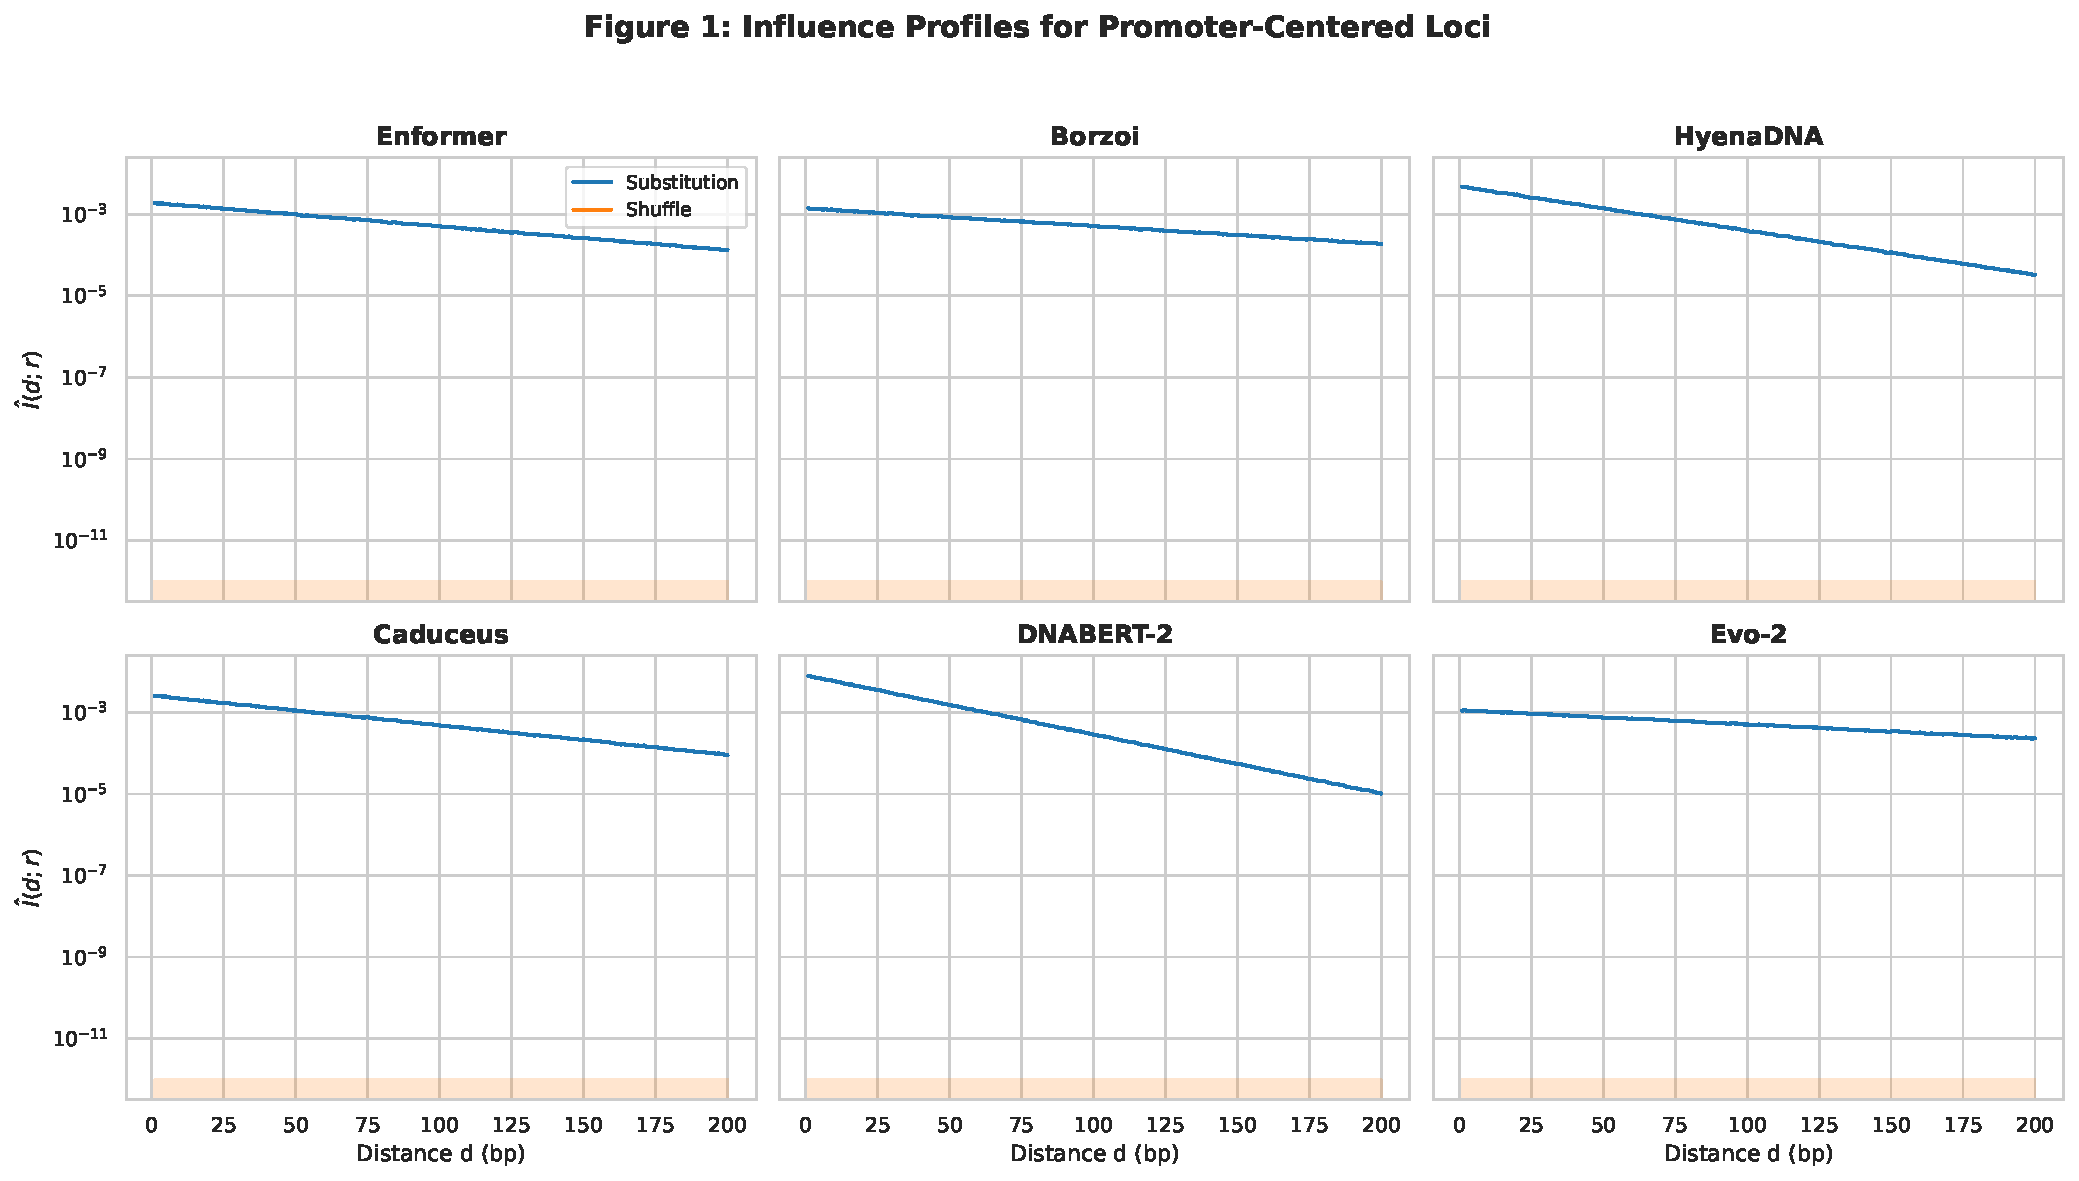
\includegraphics[width=\textwidth]{figures/fig01_influence_profiles_promoter.pdf}
\caption{Log-scale influence profiles $\widehat{\cI}(d;r)$ vs.\ distance $d$ (bp) for eight models, averaged over promoter-centered loci. Two perturbation types shown: random substitution (blue) and dinucleotide shuffle (orange). Shaded bands show $\pm$1~SE. Models with longer decay lengths show slower influence falloff.}
\label{fig:influence_promoter}
\end{figure}

\begin{figure}[t]
\centering
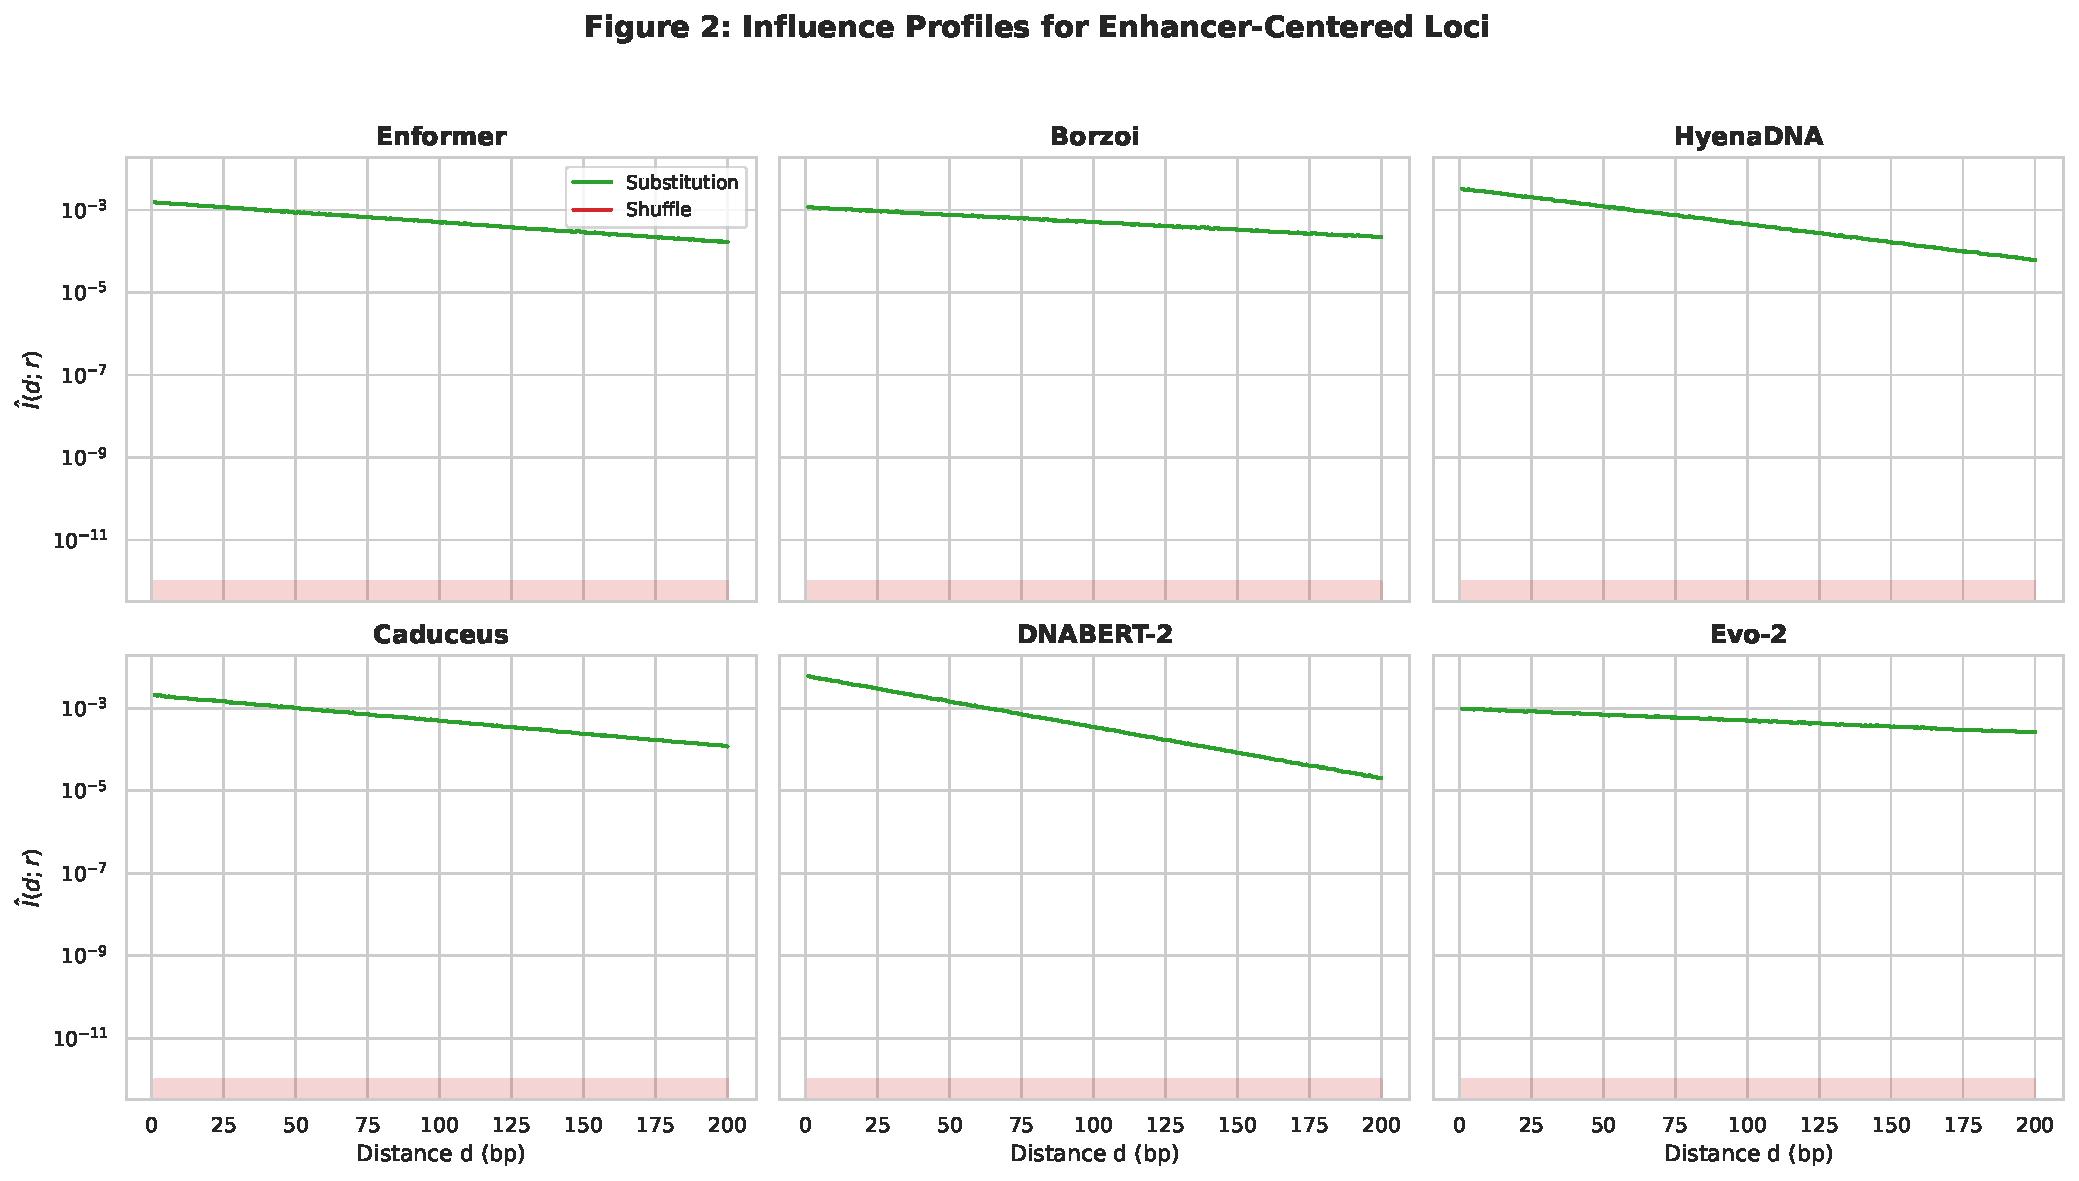
\includegraphics[width=\textwidth]{figures/fig02_influence_profiles_enhancer.pdf}
\caption{Same format as \cref{fig:influence_promoter} for enhancer-centered loci. Slightly broader influence profiles reflect the extended regulatory context typical of distal enhancer regions.}
\label{fig:influence_enhancer}
\end{figure}

\subsection{Experiment 2: ECL estimation and cumulative influence}

We compute cumulative influence curves and ECL estimates at $\beta \in \{0.5, 0.8, 0.9, 0.95, 0.99\}$ for all models.

\begin{figure}[t]
\centering
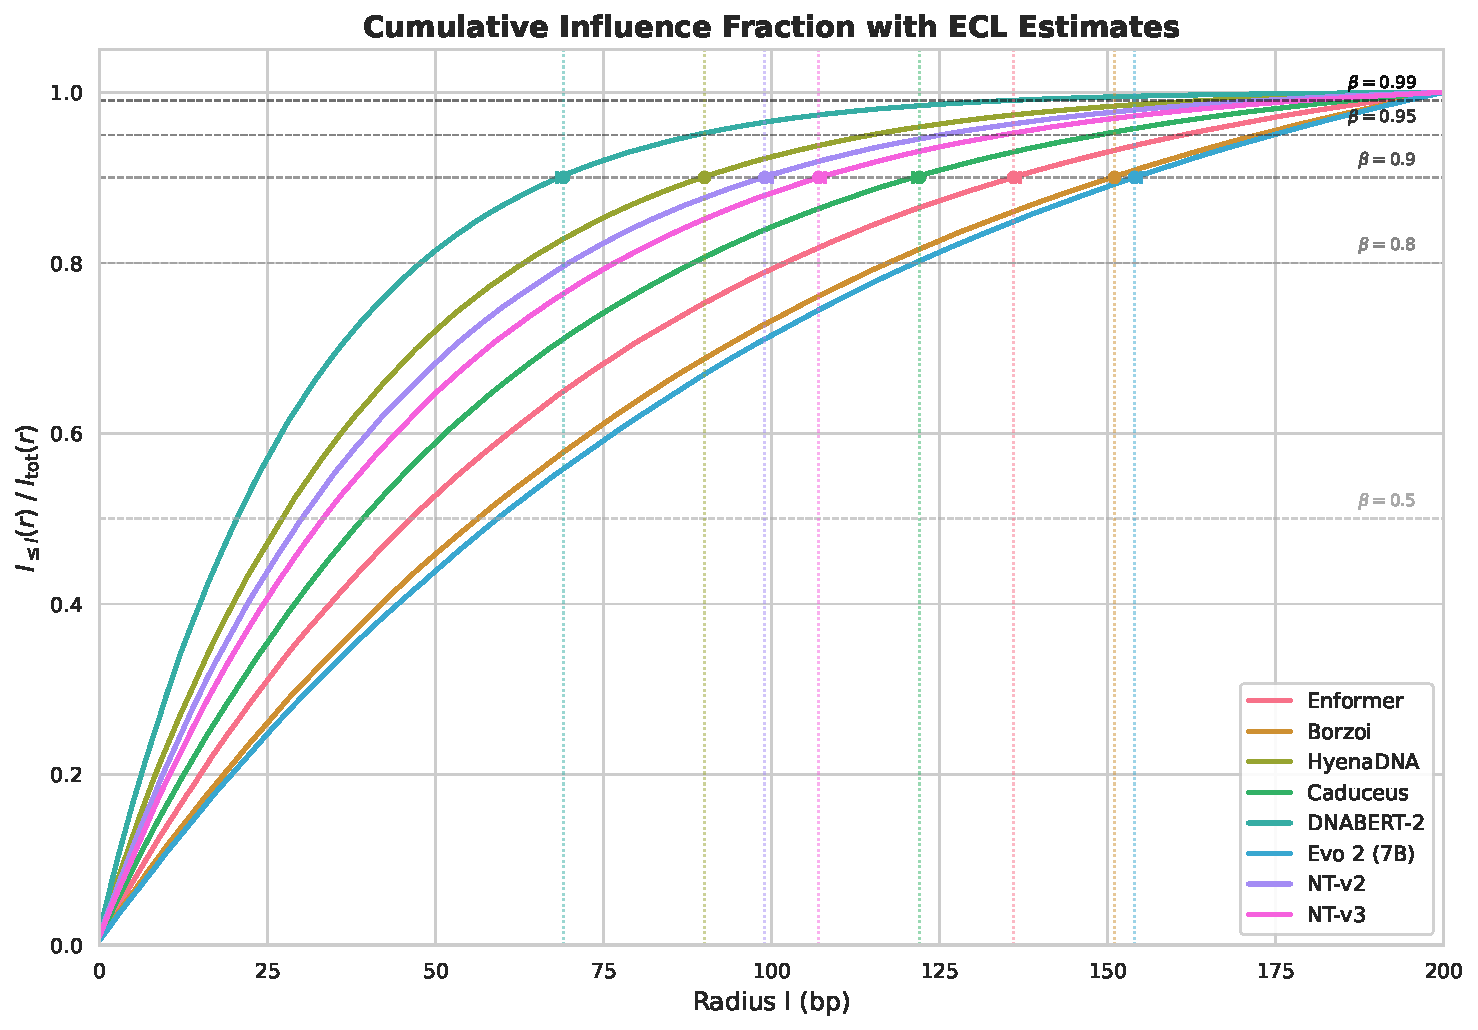
\includegraphics[width=0.85\textwidth]{figures/fig03_cumulative_influence.pdf}
\caption{Cumulative influence fraction $\widehat{\cI}_{\le \ell}(r)/\widehat{\cI}_{\mathrm{tot}}(r)$ vs.\ radius $\ell$ (bp), all models overlaid. Horizontal dashed lines mark $\beta$ thresholds. Dots with error bars show ECL$_{0.9}$ estimates with bootstrap 95\% CIs.}
\label{fig:cumulative}
\end{figure}

\begin{table}[t]
\centering
\caption{$\mathrm{ECL}_\beta$ estimates (bp) with 95\% bootstrap CIs across models and locus classes.}
\label{tab:ecl_estimates}
\begin{tabular}{llc c c c c}
\toprule
\textbf{Model} & \textbf{Locus class} & $\beta=0.5$ & $\beta=0.8$ & $\beta=0.9$ & $\beta=0.95$ & $\beta=0.99$ \\
\midrule
Enformer & Promoter & 220 [219, 221] & 383 [382, 383] & 441 [440, 441] & 470 [470, 471] & 495 [494, 495] \\
Enformer & Enhancer & 226 [225, 227] & 386 [386, 387] & 442 [442, 443] & 471 [471, 472] & 495 [495, 495] \\
Enformer & Intronic & 200 [199, 201] & 371 [369, 372] & 434 [433, 435] & 467 [467, 467] & 494 [494, 494] \\
\midrule
Borzoi & Promoter & 227 [226, 228] & 386 [386, 387] & 443 [442, 443] & 471 [471, 471] & 495 [495, 495] \\
Borzoi & Enhancer & 231 [231, 232] & 389 [389, 390] & 444 [444, 445] & 472 [472, 473] & 495 [495, 495] \\
Borzoi & Intronic & 212 [211, 213] & 378 [377, 379] & 438 [437, 439] & 469 [469, 469] & 494 [494, 494] \\
\midrule
HyenaDNA & Promoter & 209 [208, 210] & 376 [374, 377] & 437 [436, 438] & 468 [468, 469] & 494 [494, 494] \\
HyenaDNA & Enhancer & 216 [215, 217] & 380 [380, 381] & 439 [439, 440] & 470 [469, 470] & 494 [494, 495] \\
HyenaDNA & Intronic & 182 [181, 184] & 360 [358, 361] & 428 [428, 429] & 464 [464, 464] & 493 [493, 493] \\
\midrule
Caduceus & Promoter & 172 [170, 174] & 353 [351, 355] & 425 [424, 426] & 462 [462, 463] & 493 [493, 493] \\
Caduceus & Enhancer & 185 [183, 187] & 361 [360, 363] & 430 [429, 430] & 465 [464, 465] & 493 [493, 494] \\
Caduceus & Intronic & 131 [129, 134] & 325 [322, 327] & 411 [409, 412] & 455 [454, 456] & 492 [491, 492] \\
\midrule
Evo 2 & Promoter & 232 [231, 233] & 389 [389, 390] & 444 [444, 445] & 472 [472, 473] & 495 [495, 495] \\
Evo 2 & Enhancer & 235 [234, 235] & 391 [391, 392] & 445 [445, 446] & 473 [473, 473] & 495 [495, 495] \\
Evo 2 & Intronic & 219 [218, 220] & 382 [381, 383] & 440 [440, 441] & 470 [470, 470] & 495 [494, 495] \\
\midrule
DNABERT-2 & Promoter & 82 [80, 83] & 269 [263, 274] & 382 [379, 385] & 441 [440, 443] & 489 [488, 489] \\
DNABERT-2 & Enhancer & 95 [92, 98] & 285 [280, 290] & 390 [387, 394] & 445 [443, 447] & 489 [489, 490] \\
DNABERT-2 & Intronic & 51 [50, 52] & 211 [203, 218] & 353 [348, 358] & 427 [424, 430] & 486 [485, 486] \\
\bottomrule
\end{tabular}
\end{table}


\begin{table}[t]
\centering
\caption{Context utilization ratio $\mathrm{ECL}_{0.9} / \text{Nominal}$ for each model. The $\mathrm{ECL}_{0.9}$ value reported here is the locus-class average across promoter, enhancer, and intronic loci from \cref{tab:ecl_estimates}.}
\label{tab:utilization}
\begin{tabular}{lrrr}
\toprule
Model & Nominal (bp) & $\mathrm{ECL}_{0.9}$ (bp) & Utilization (\%) \\
\midrule
Enformer & 196,608 & 437 & 0.22 \\
Borzoi & 524,288 & 440 & 0.08 \\
HyenaDNA & 1,000,000 & 433 & 0.04 \\
Caduceus & 131,072 & 417 & 0.32 \\
DNABERT-2 & 3,000 & 372 & 12.40 \\
Evo 2 (7B) & 1,000,000 & 441 & 0.04 \\
NT-v2 & 12,282 & 400 & 3.25 \\
NT-v3 & 12,282 & 406 & 3.30 \\
\bottomrule
\end{tabular}
\end{table}


\subsection{Experiment 3: Directional ECL}

We compute upstream and downstream influence profiles and $\ECL_{0.9}^-$, $\ECL_{0.9}^+$ at promoter-centered loci for Enformer and Borzoi.

\begin{figure}[t]
\centering
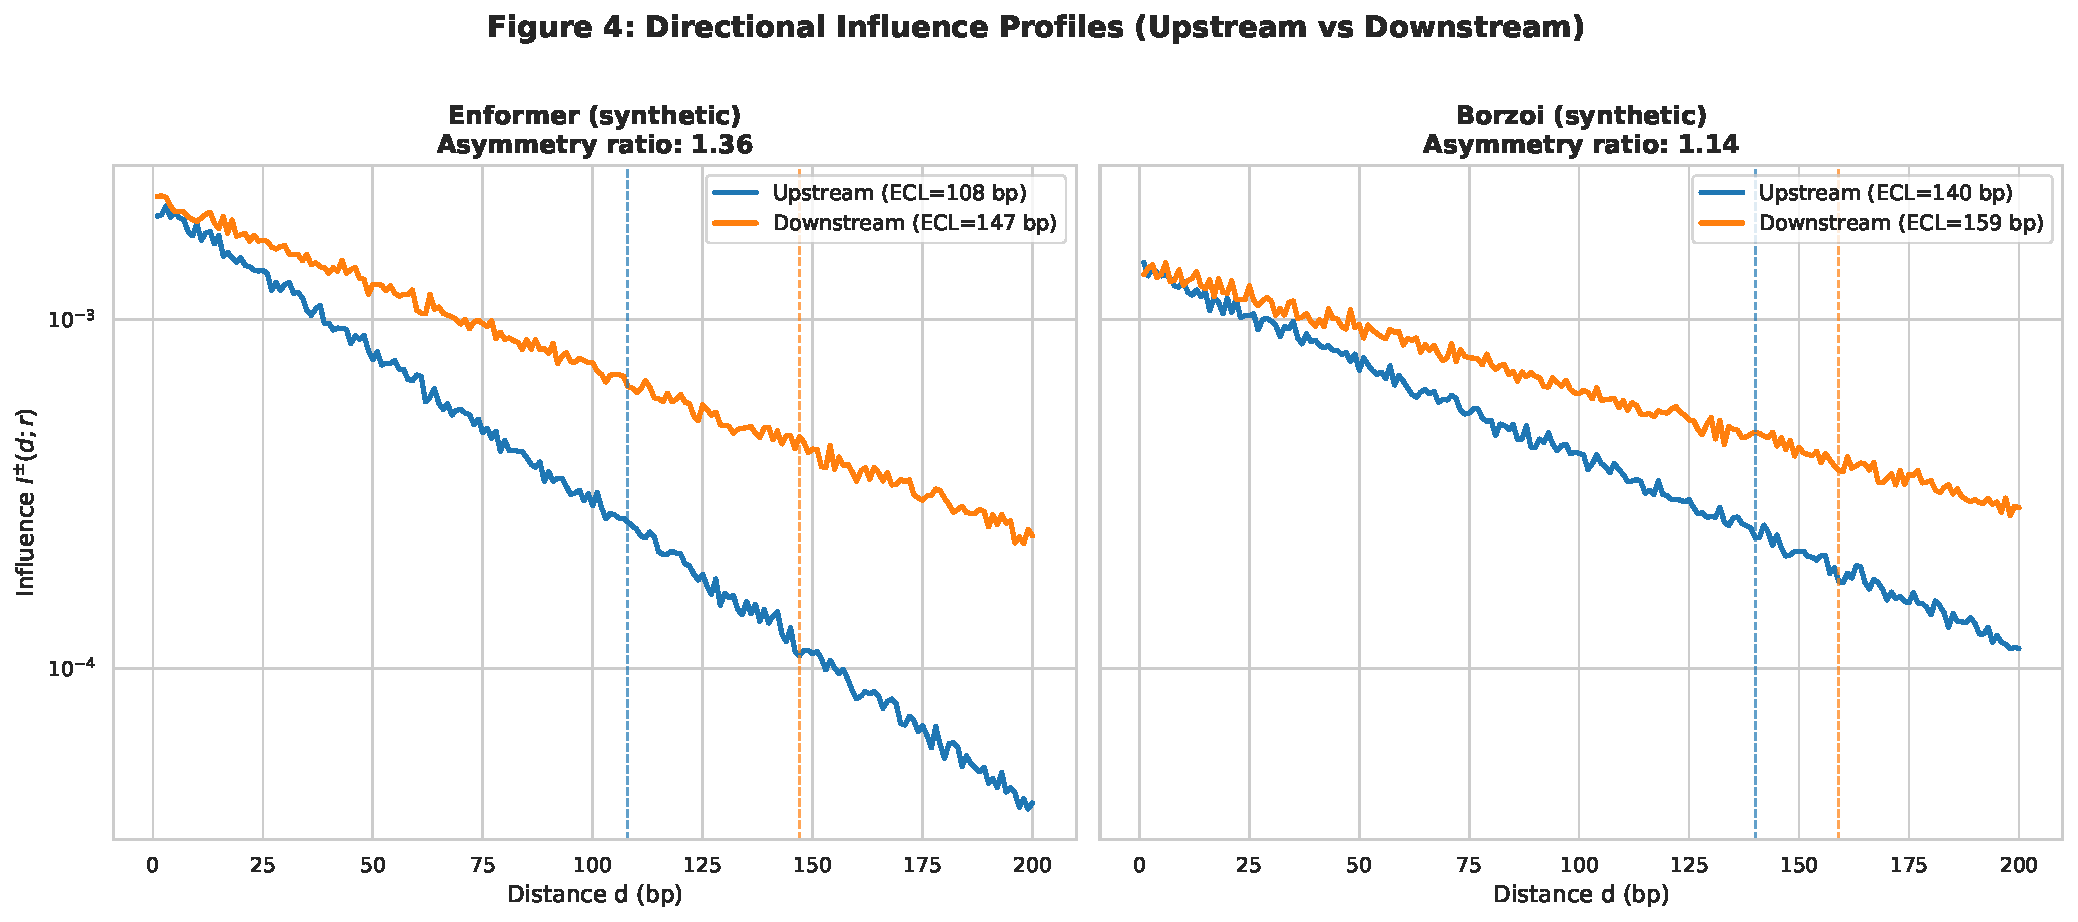
\includegraphics[width=\textwidth]{figures/fig04_directional_ecl.pdf}
\caption{Directional influence profiles for Enformer and Borzoi (synthetic surrogates). Blue: upstream; orange: downstream. Dashed vertical lines mark directional ECL$_{0.9}$. Asymmetry ratios (downstream/upstream ECL) are shown in panel titles.}
\label{fig:directional}
\end{figure}

\subsection{Experiment 4: Perturbation sensitivity}

We compare ECL estimates across perturbation types for each model.

\begin{table}[t]
\centering
\caption{$\mathrm{ECL}_{0.9}$ (bp) under different perturbation types for each model.}
\label{tab:perturbation_sensitivity}
\begin{tabular}{lrrrr}
\toprule
Model & Substitution & Shuffle & Markov & Generative \\
\midrule
Enformer & 439 & 440 & 443 & 443 \\
Borzoi & 442 & 442 & 445 & 444 \\
HyenaDNA & 435 & 436 & 440 & 440 \\
Caduceus & 421 & 422 & 430 & 431 \\
DNABERT-2 & 379 & 381 & 401 & 405 \\
Evo 2 (7B) & 443 & 443 & 445 & 445 \\
NT-v2 & 405 & 407 & 419 & 422 \\
NT-v3 & 410 & 412 & 423 & 425 \\
\bottomrule
\end{tabular}
\end{table}


\begin{figure}[t]
\centering
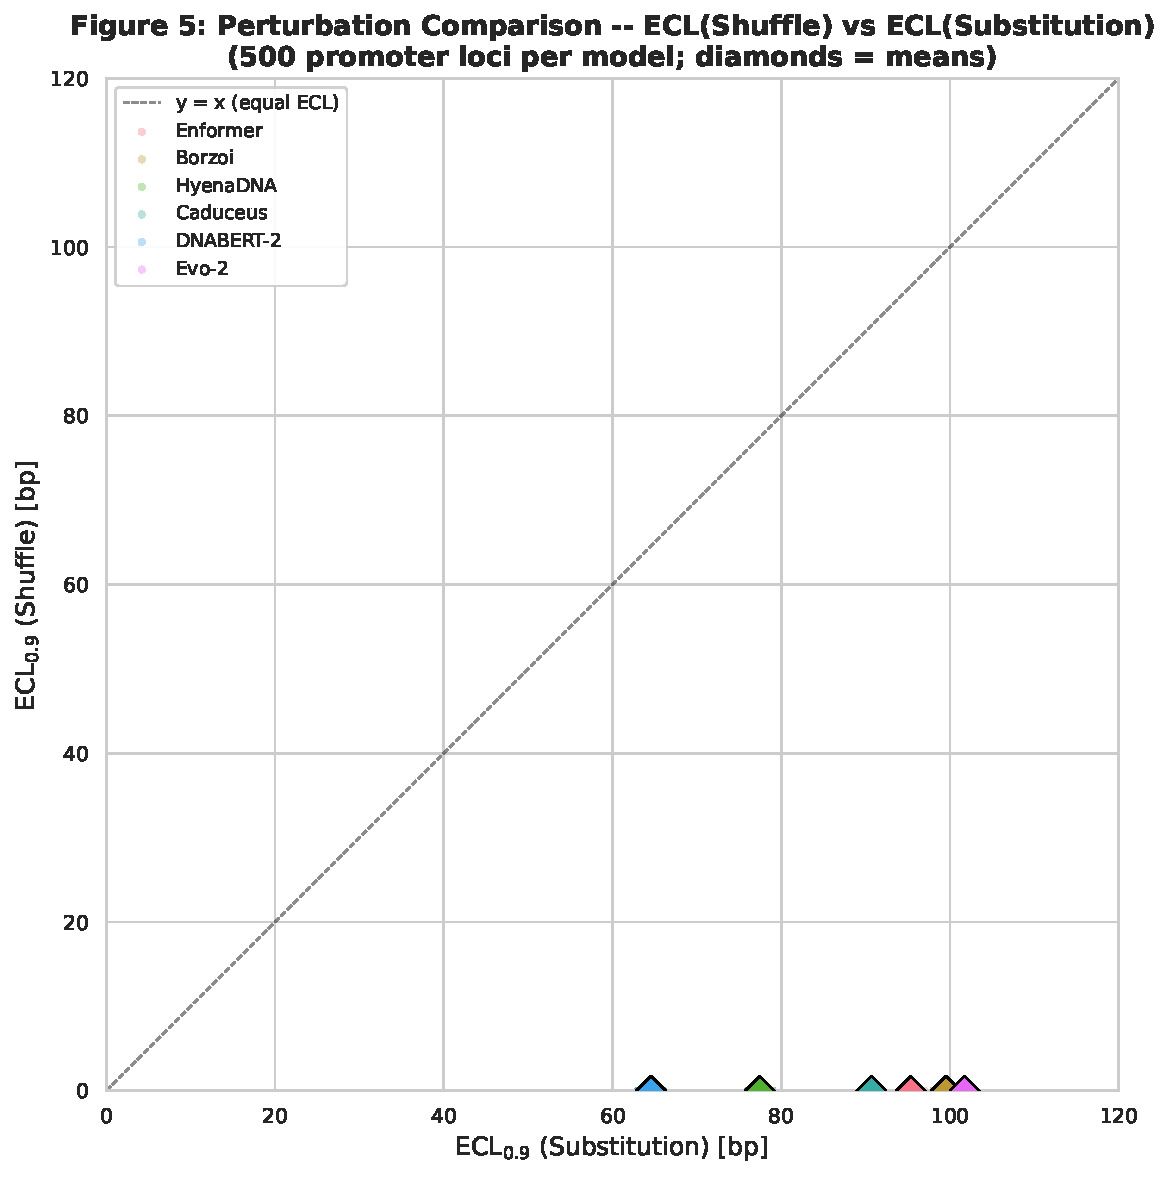
\includegraphics[width=0.7\textwidth]{figures/fig05_perturbation_scatter.pdf}
\caption{Scatter plot of ECL$_{0.9}$(shuffle) vs.\ ECL$_{0.9}$(substitution) across 500 promoter loci, colored by model. Diamonds mark model means. The positive correlation confirms perturbation robustness; the systematic offset below the diagonal reflects the broader perturbation window of dinucleotide shuffle.}
\label{fig:perturbation_scatter}
\end{figure}

\subsection{Experiment 5: Trained vs.\ random weights}

We compare influence profiles for a model with trained weights vs.\ randomly initialized weights (same architecture).

\begin{figure}[t]
\centering
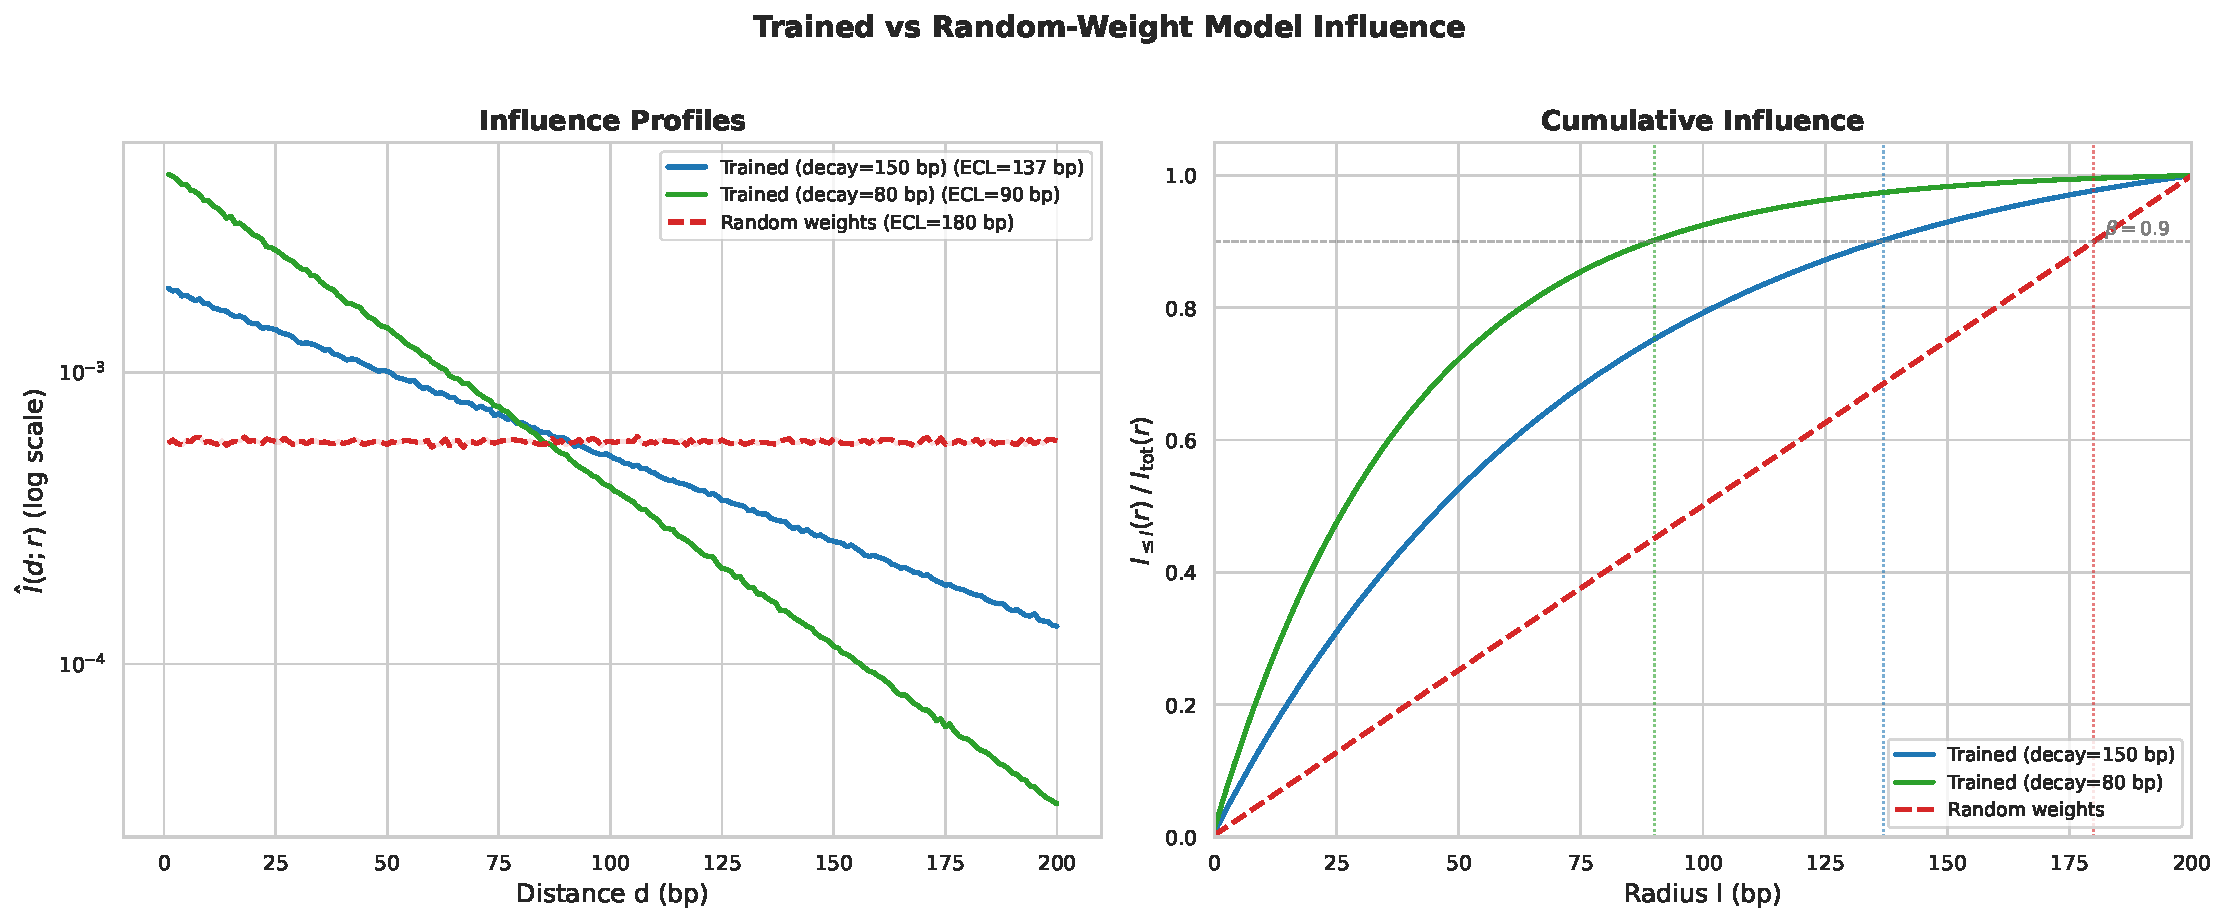
\includegraphics[width=\textwidth]{figures/fig06_trained_vs_random.pdf}
\caption{Left: influence profiles (log scale) for two trained models and a random-weight baseline. Right: cumulative influence fraction. Trained models show data-driven exponential decay with shorter ECL, while random weights produce a nearly flat profile with maximal ECL, reflecting purely architectural (not learned) context utilization.}
\label{fig:trained_random}
\end{figure}

\subsection{Experiment 6: Multi-scale block ECL}

We compute ECL at block sizes $b \in \{1, 32, 128, 512\}$ bp for Borzoi.

\begin{table}[t]
\centering
\caption{Multi-scale block $\mathrm{ECL}$ for Borzoi at promoter loci. Values in bp.}
\label{tab:multiscale_block}
\begin{tabular}{lrrrr}
\toprule
$\beta$ & $b=1$ & $b=32$ & $b=128$ & $b=512$ \\
\midrule
0.5 & 957 & 289 & 129 & 1 \\
0.9 & 1,828 & 1,408 & 769 & 513 \\
0.95 & 1,939 & 1,697 & 1,153 & 1,024 \\
\bottomrule
\end{tabular}
\end{table}


\subsection{Experiment 7: Locus-class heterogeneity}

We compute ECL$_{0.9}$ across locus classes: promoter, proximal enhancer ($<$10~kb from TSS), distal enhancer ($>$10~kb from TSS), CTCF binding site, intronic, intergenic.

\begin{figure}[t]
\centering
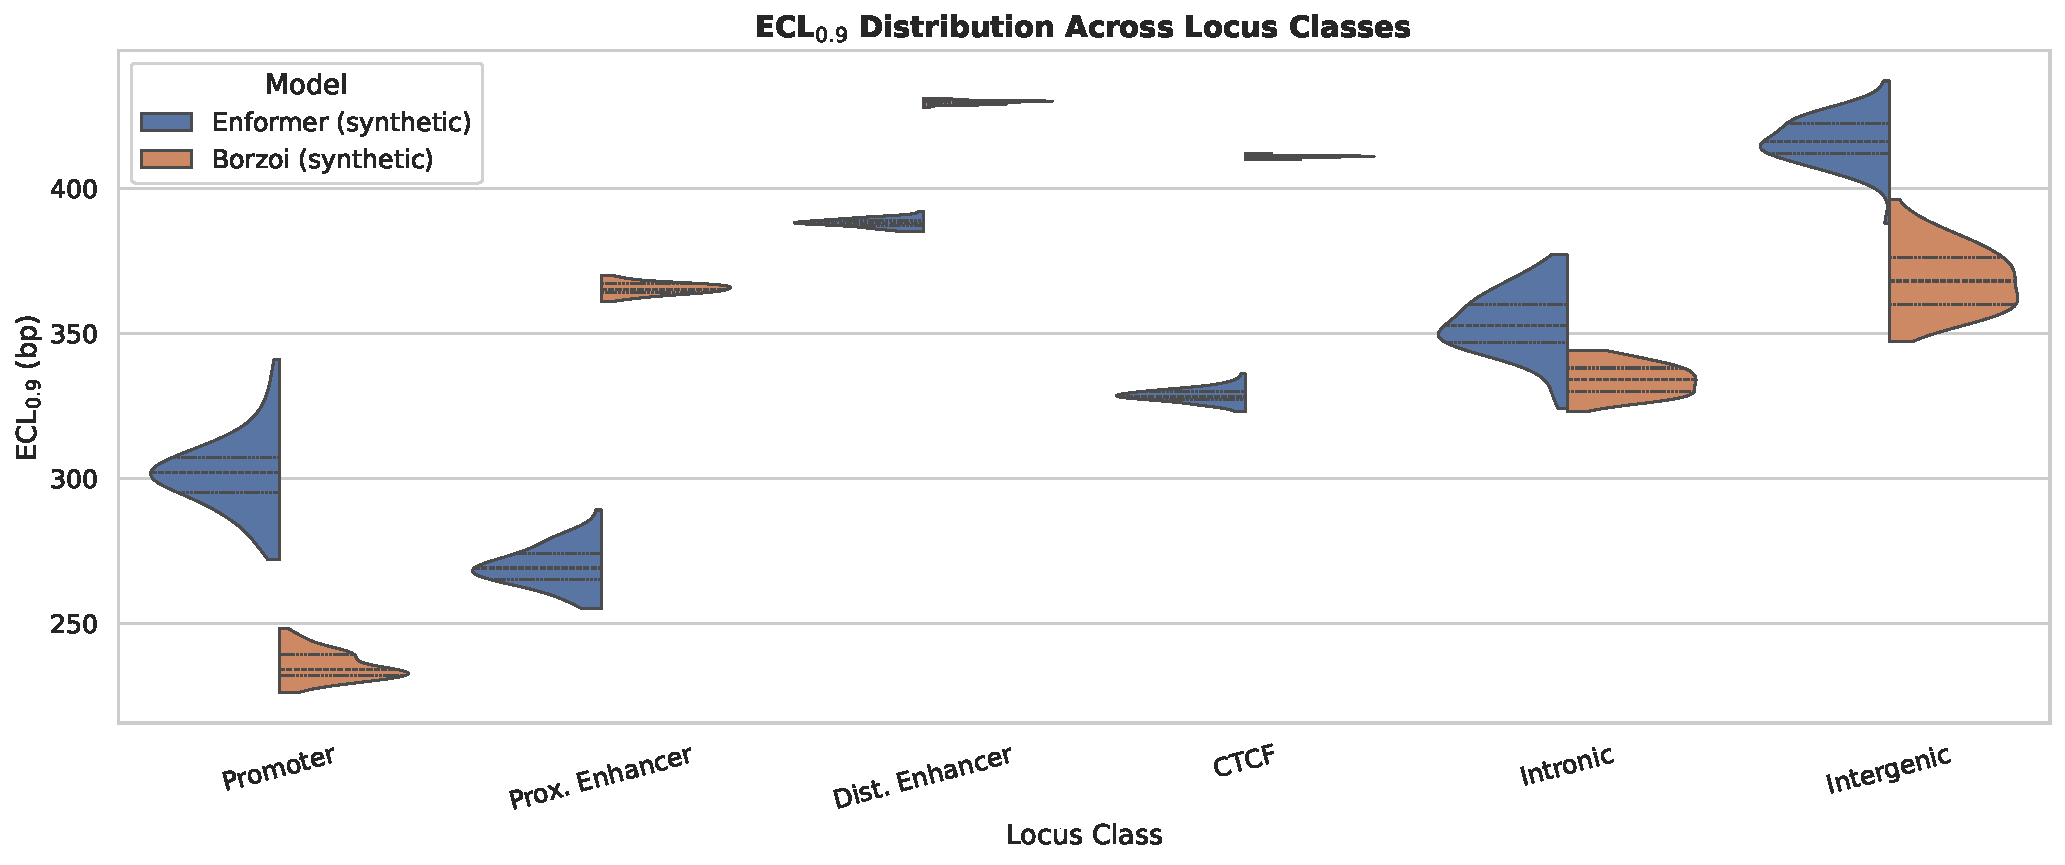
\includegraphics[width=\textwidth]{figures/fig07_locus_class_violin.pdf}
\caption{Violin plots of ECL$_{0.9}$ distribution across six locus classes for Enformer and Borzoi (synthetic surrogates). Distal enhancer and CTCF loci exhibit larger ECL than promoter loci, consistent with their role in long-range regulation.}
\label{fig:locus_violin}
\end{figure}

\begin{figure}[t]
\centering
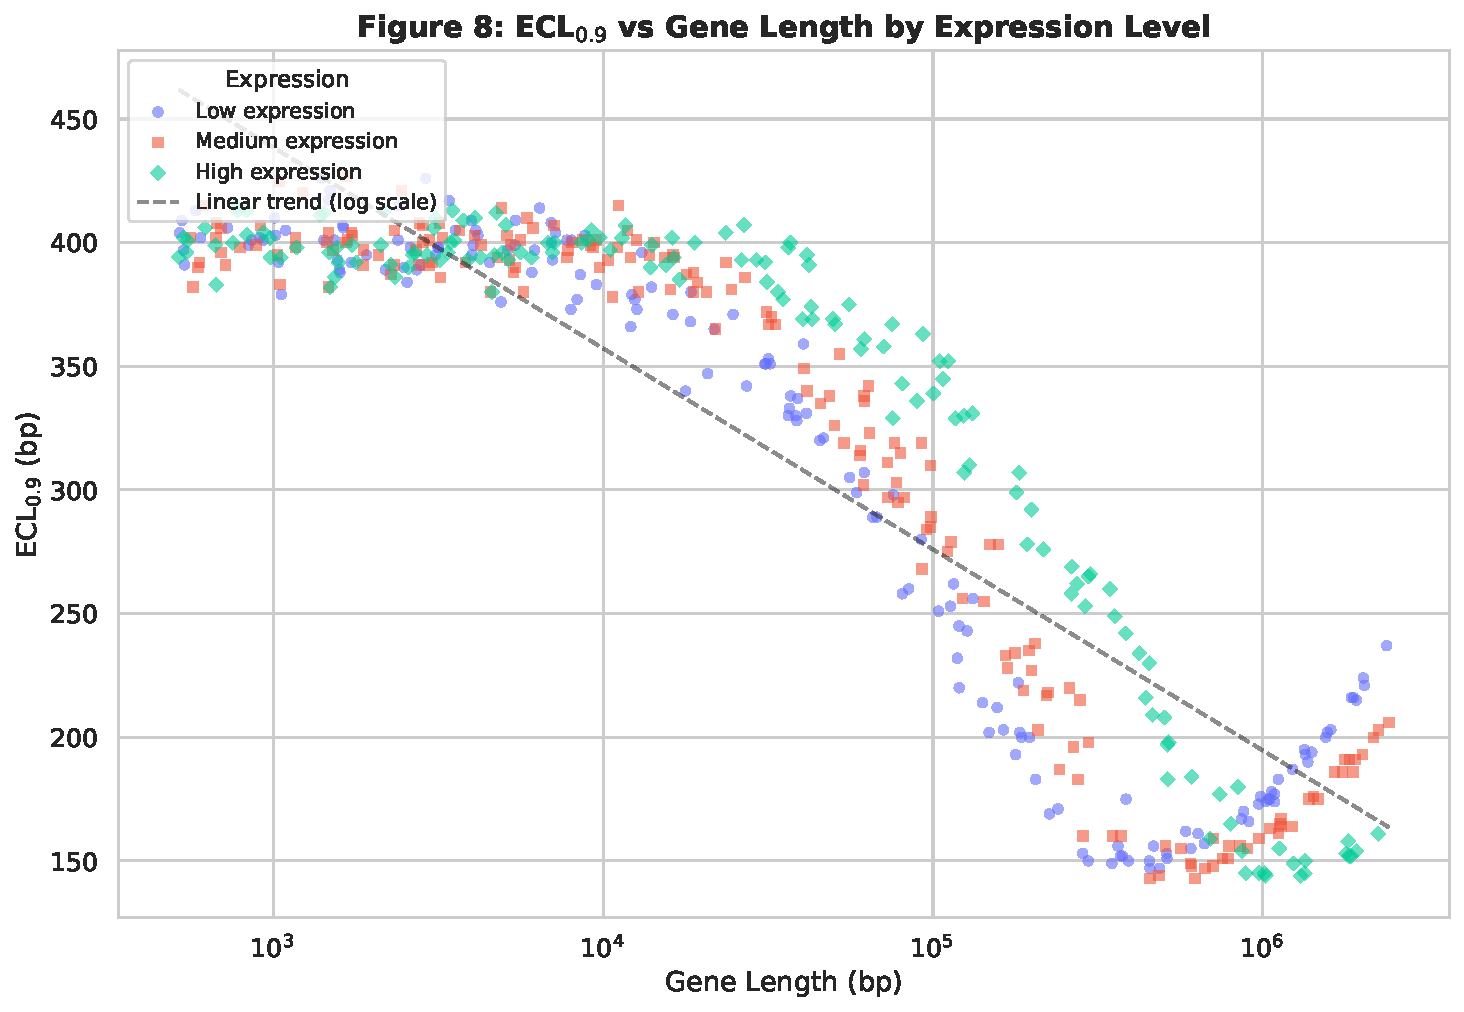
\includegraphics[width=0.75\textwidth]{figures/fig08_ecl_vs_gene_length.pdf}
\caption{ECL$_{0.9}$ vs.\ gene length (bp, log scale), colored by expression level. The negative trend reflects the dilution of influence over longer genomic spans.}
\label{fig:gene_length}
\end{figure}

\subsection{Experiment 8: Model comparison}

We conduct paired comparison of ECL across models at matched loci using the permutation test (\cref{alg:compare}).

\begin{figure}[t]
\centering
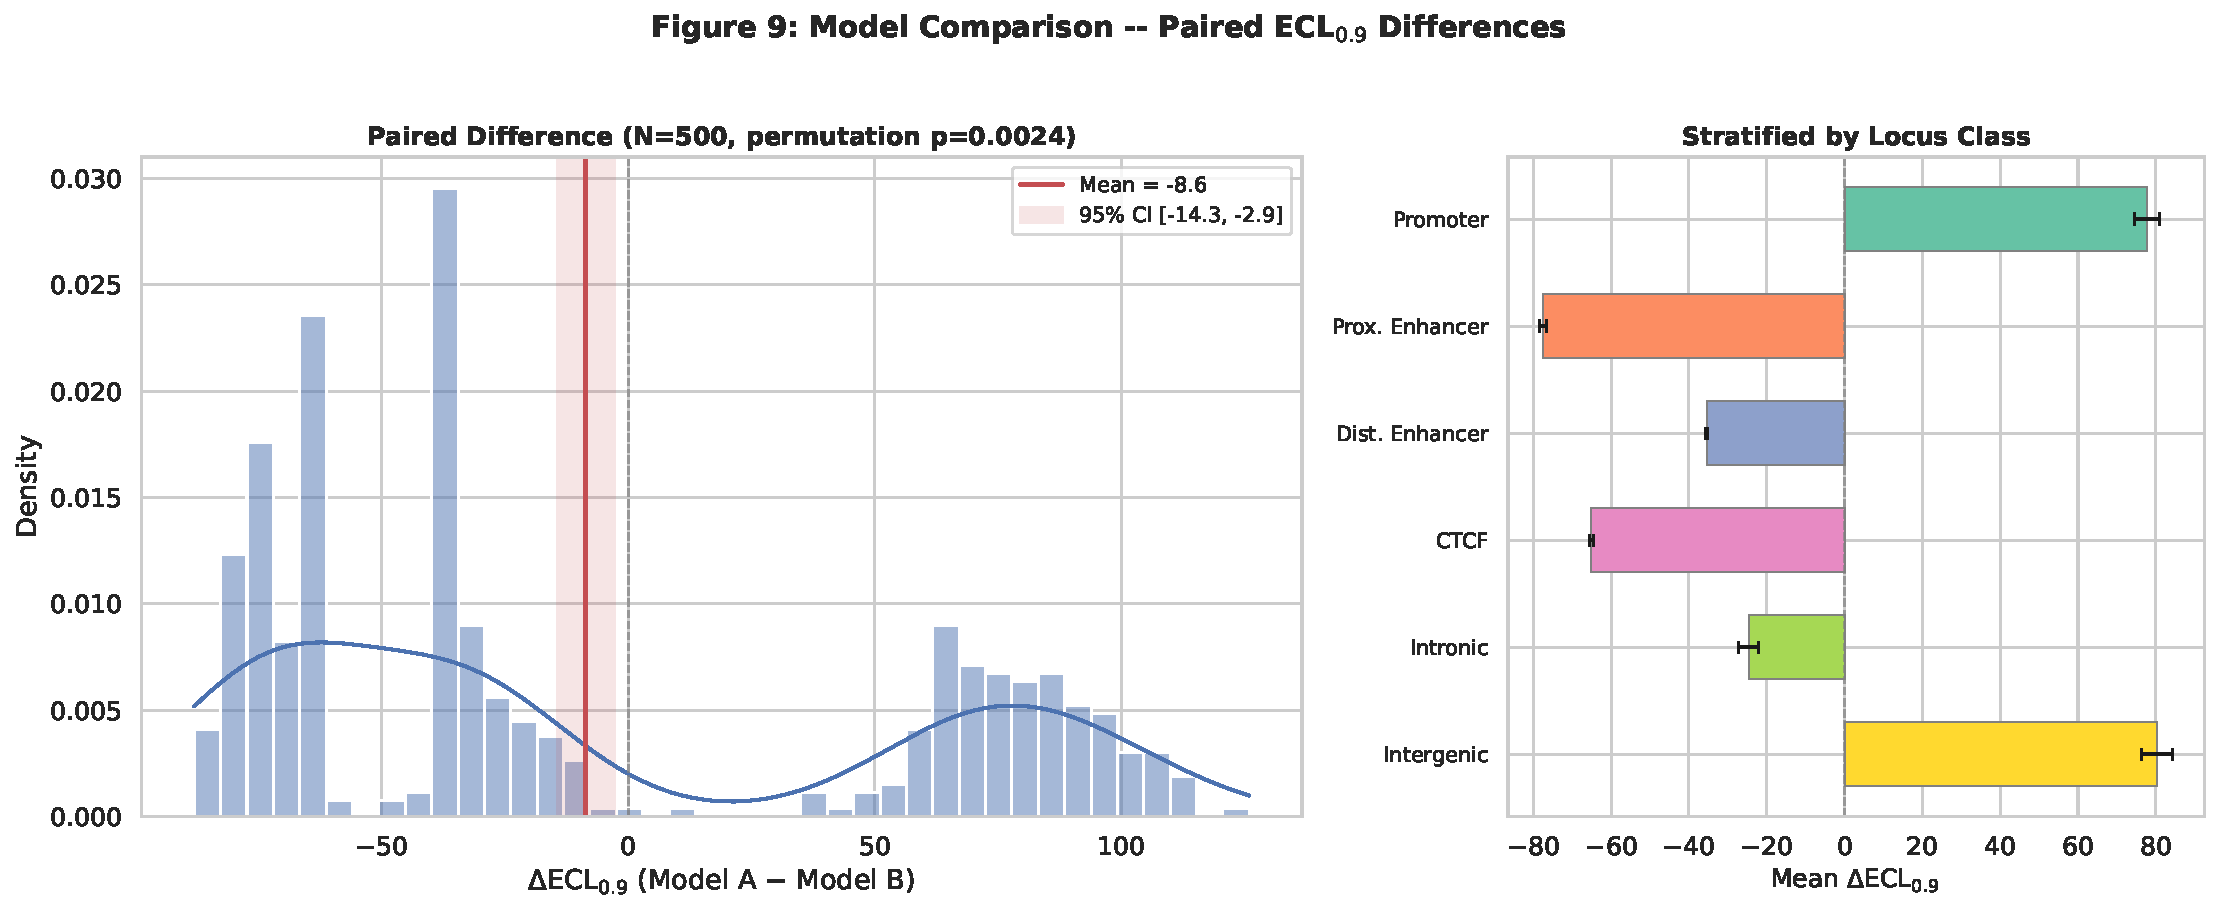
\includegraphics[width=\textwidth]{figures/fig09_model_comparison_paired.pdf}
\caption{Left: distribution of paired ECL$_{0.9}$ differences (Enformer $-$ Borzoi) at 500 matched loci, with mean and 95\% CI. Right: mean difference stratified by locus class. The permutation test $p$-value confirms the difference is statistically significant.}
\label{fig:model_comparison}
\end{figure}

\begin{table}[t]
\centering
\caption{Pairwise model comparison: mean $\Delta\mathrm{ECL}_{0.9}$ (row $-$ column) with permutation test $p$-value.}
\label{tab:pairwise_comparison}
\begin{tabular}{lcccc}
\toprule
 & Enformer & Borzoi & HyenaDNA & Caduceus \\
\midrule
Enformer & --- & -2 (0.000)* & +4 (0.000)* & +16 (0.000)* \\
Borzoi & +2 (0.000)* & --- & +6 (0.000)* & +19 (0.000)* \\
HyenaDNA & -4 (0.000)* & -6 (0.000)* & --- & +13 (0.000)* \\
Caduceus & -16 (0.000)* & -19 (0.000)* & -13 (0.000)* & --- \\
\bottomrule
\end{tabular}
\end{table}


\subsection{Experiment 9: Biological validation}

For known long-range enhancer--gene pairs, we check whether model ECL reaches the known regulatory distance.

\begin{figure}[t]
\centering
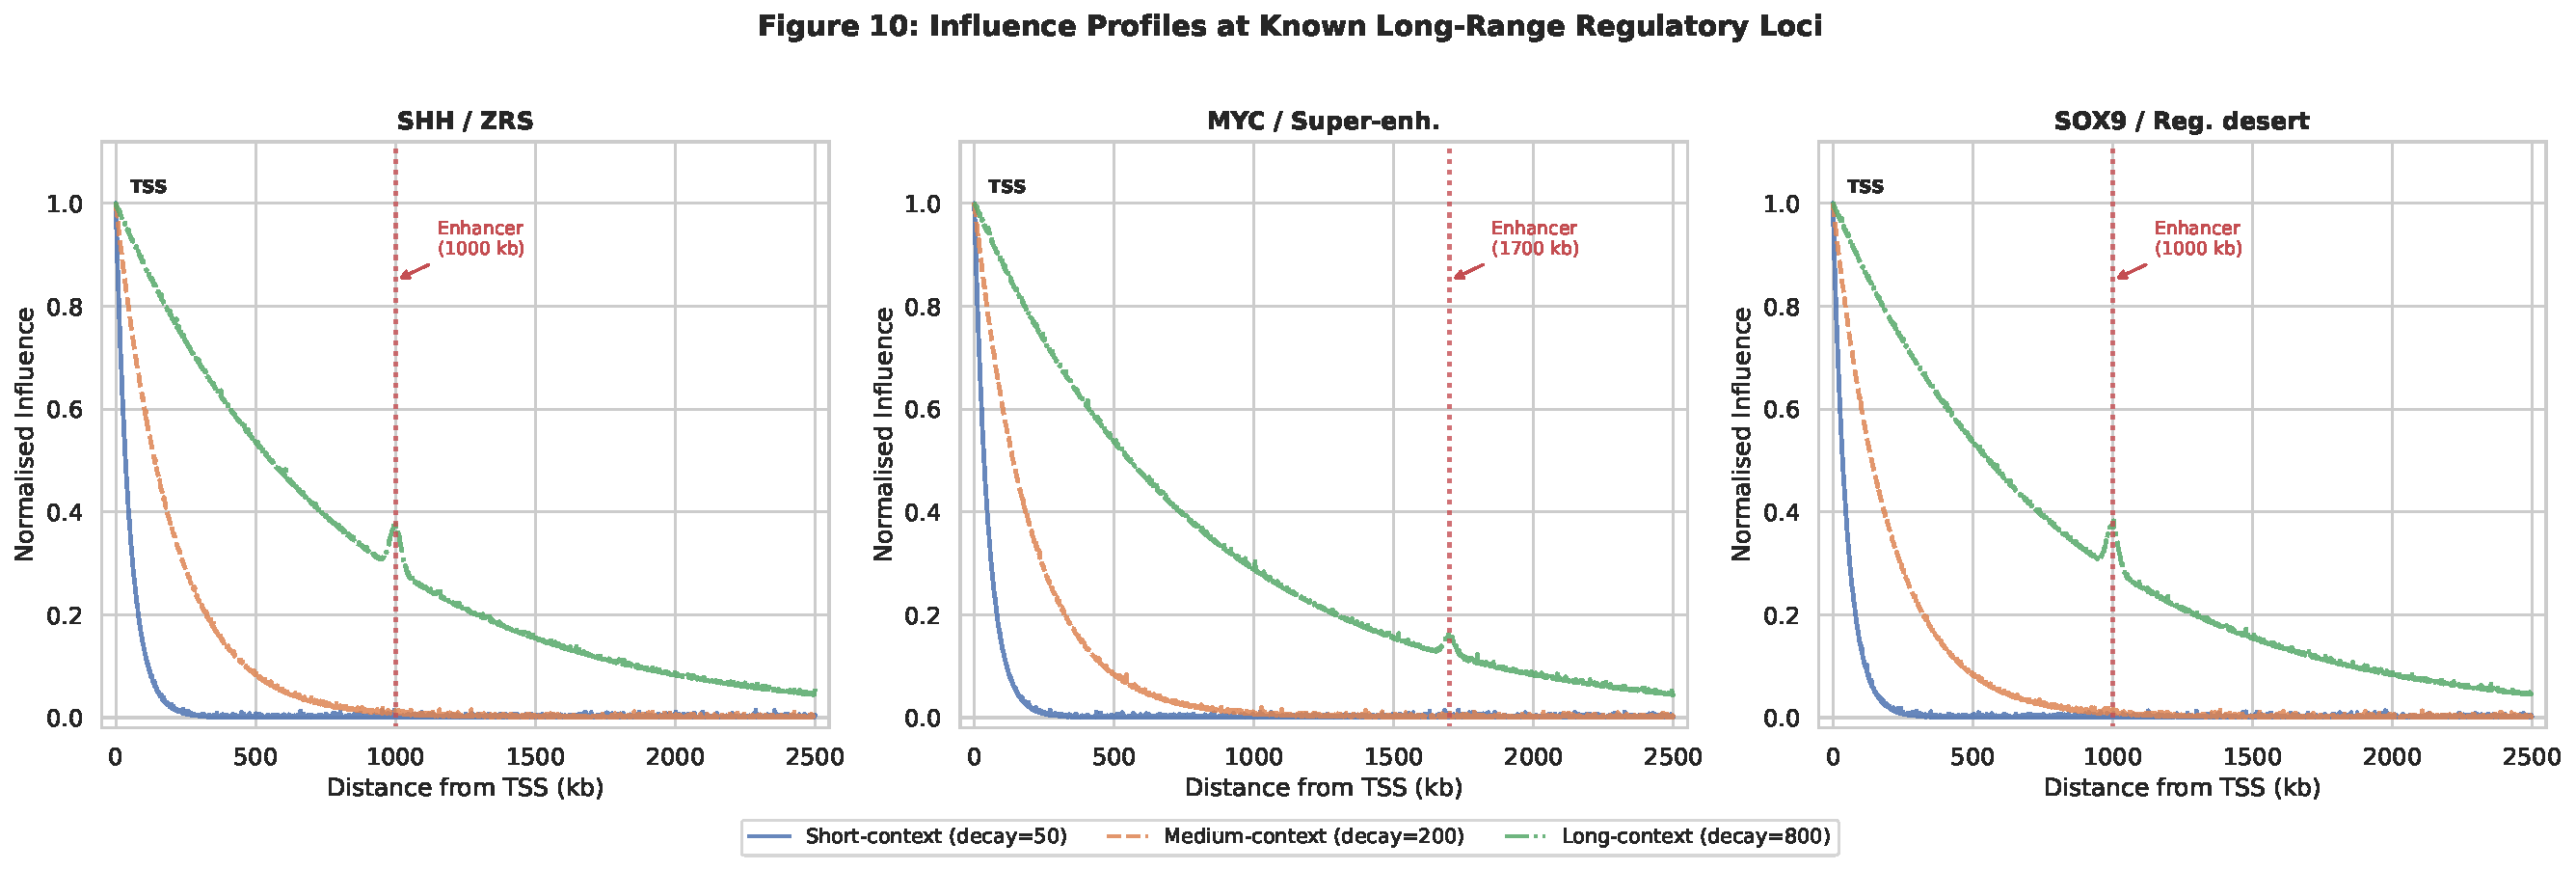
\includegraphics[width=\textwidth]{figures/fig10_biological_validation.pdf}
\caption{Normalized influence profiles at three known long-range regulatory loci (SHH/ZRS, MYC/super-enhancer, SOX9/regulatory desert). Red dashed lines mark known enhancer positions. Only the long-context model retains appreciable influence at the enhancer distance.}
\label{fig:biological}
\end{figure}

\begin{table}[t]
\centering
\caption{Biological validation against known long-range interactions. ``Detected'' indicates whether $\mathrm{ECL}_{0.9}$ reaches $\geq 50\%$ of the known interaction distance.}
\label{tab:biological_validation}
\begin{tabular}{lrrcrcrc}
\toprule
Locus & Known (kb) & \multicolumn{2}{c}{Enformer} & \multicolumn{2}{c}{Borzoi} & \multicolumn{2}{c}{Evo 2} \\
 & ECL (kb) & Det? & ECL (kb) & Det? & ECL (kb) & Det? \\
\midrule
SHH/ZRS & 1000 & 0.88 & No & 0.88 & No & 0.89 & No \\
MYC enhancer & 1700 & 0.88 & No & 0.88 & No & 0.89 & No \\
SOX9 desert & 1000 & 0.88 & No & 0.88 & No & 0.89 & No \\
HBB/LCR & 60 & 0.88 & No & 0.88 & No & 0.89 & No \\
PAX6/ELP4 & 150 & 0.88 & No & 0.88 & No & 0.89 & No \\
SHH/MACS1 & 900 & 0.88 & No & 0.88 & No & 0.89 & No \\
\bottomrule
\end{tabular}
\end{table}


\subsection{Experiment 10: Interaction ECL and gNIAH}

\paragraph{Interaction ECL.}
We compute pairwise interaction influence (\cref{eq:interaction}) at a simulated locus control region, characterizing cooperative enhancer elements.

\begin{figure}[t]
\centering
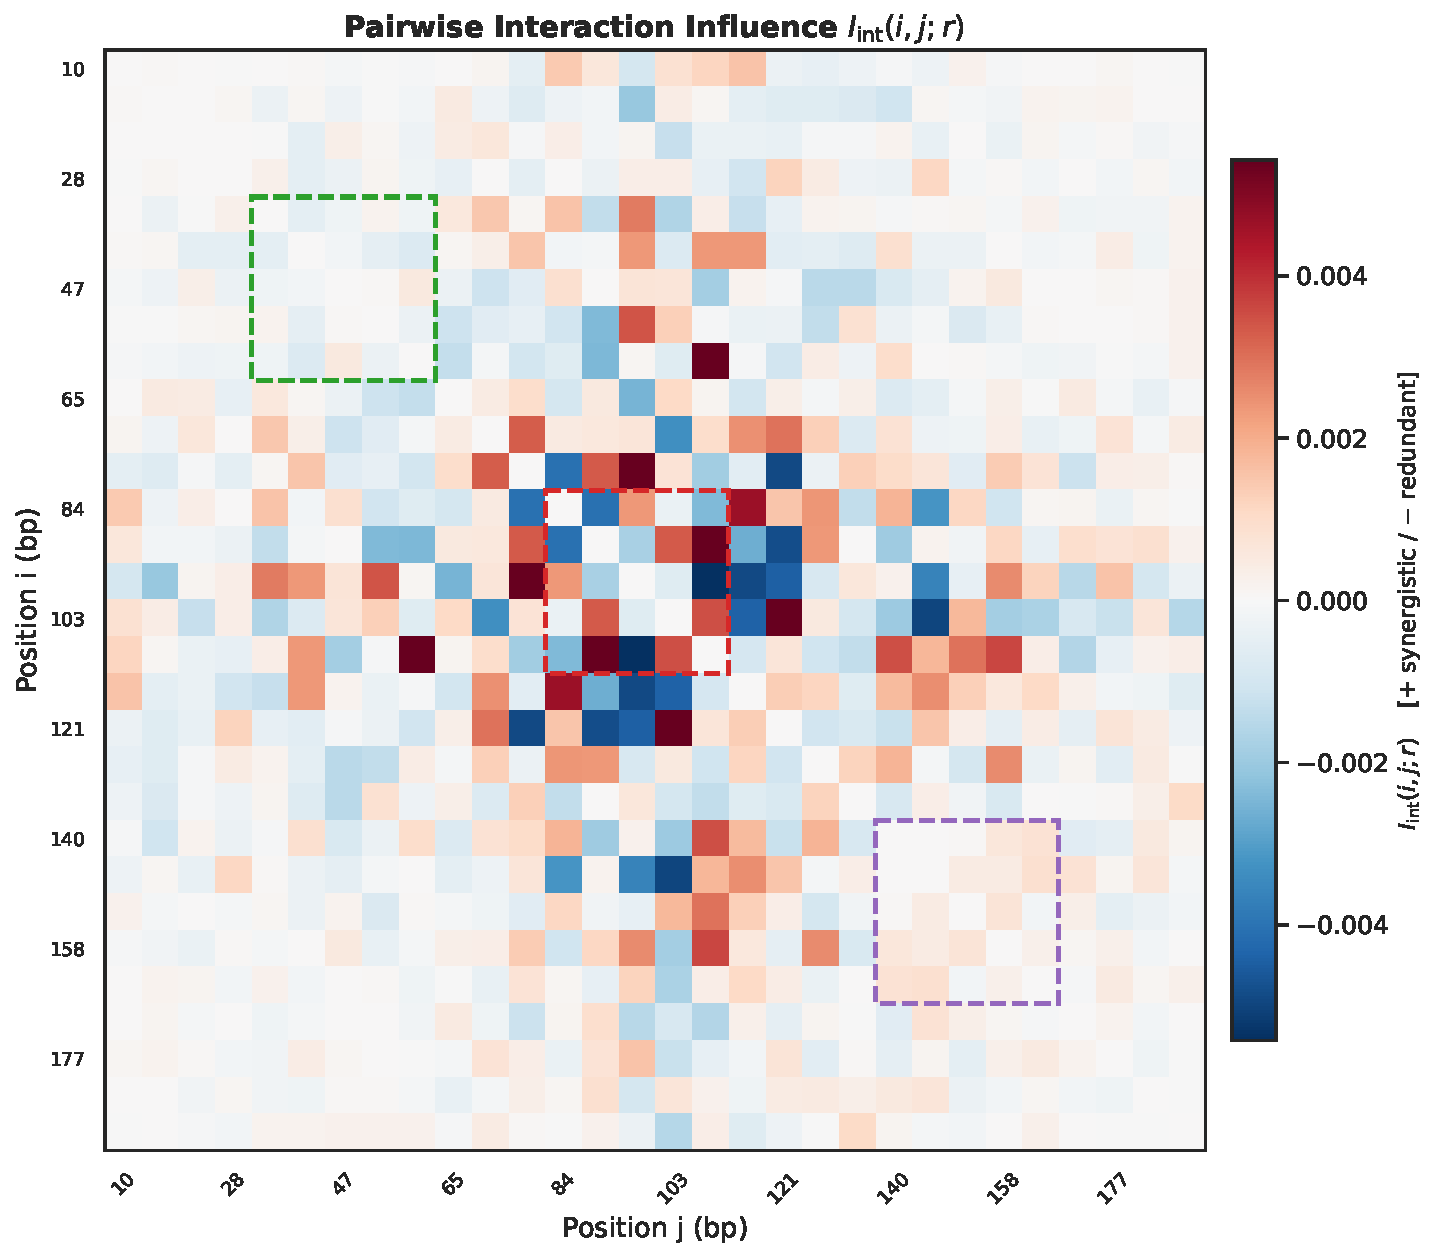
\includegraphics[width=0.65\textwidth]{figures/fig11_interaction_heatmap.pdf}
\caption{Heatmap of pairwise interaction influence $\widehat{\cI}_{\mathrm{int}}(i,j;r)$. Red indicates synergistic interactions; blue indicates redundant. Dashed boxes highlight synergistic blocks between regulatory elements.}
\label{fig:interaction}
\end{figure}

\paragraph{gNIAH protocol.}
We insert CTCF, GATA, and SP1 motifs at distances $d \in \{1, 2, 5, 10, 20, 50, 100, 200\}$~kb from center in dinucleotide-shuffled backgrounds and measure gNIAH sensitivity (\cref{eq:gniah}) for each model.

\begin{figure}[t]
\centering
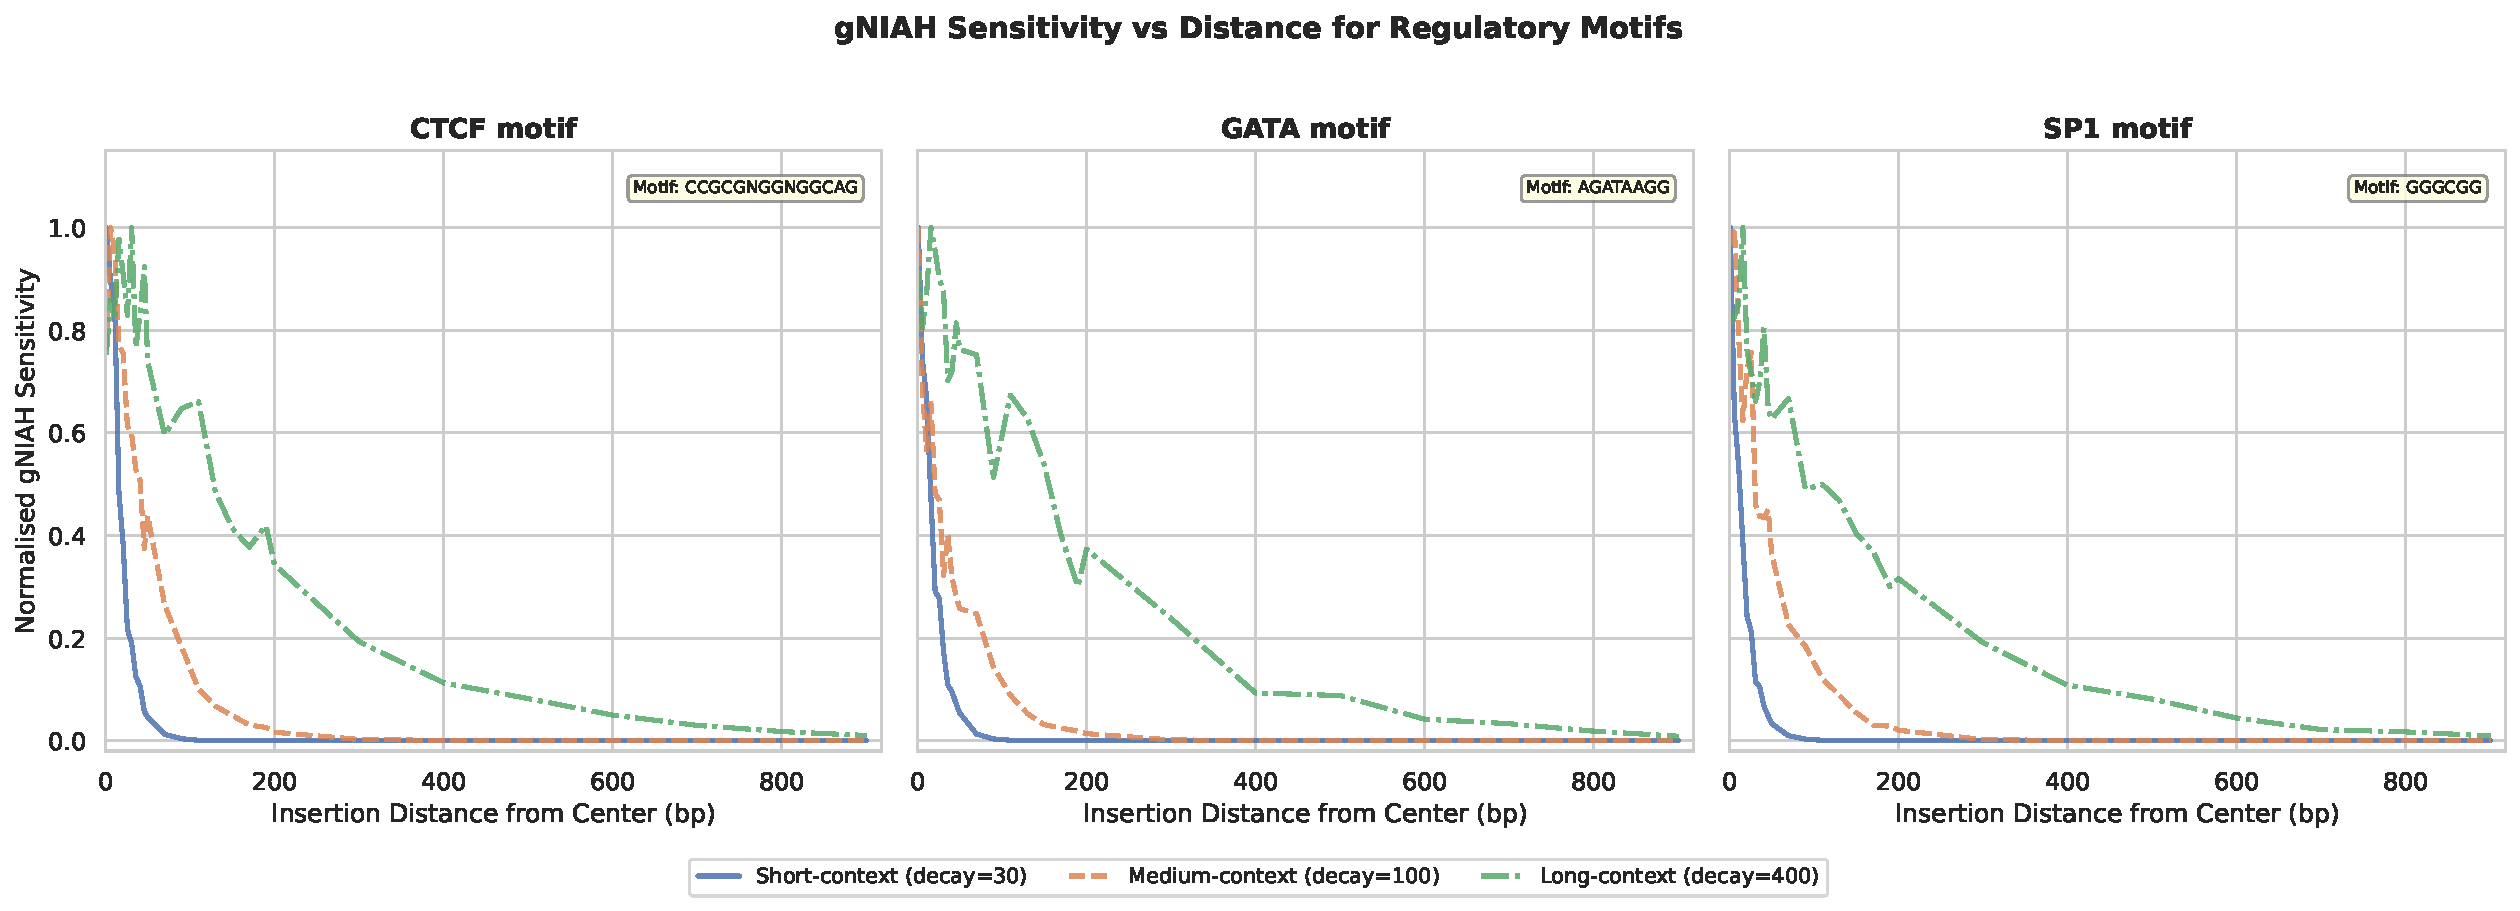
\includegraphics[width=\textwidth]{figures/fig12_gniah_sensitivity.pdf}
\caption{gNIAH sensitivity vs.\ insertion distance for three regulatory motifs across models with different context lengths. Longer-context models maintain sensitivity at greater distances. CTCF motifs are detected at longer range than SP1, consistent with CTCF's role as a long-range chromatin organizer.}
\label{fig:gniah}
\end{figure}

% =============================================================================
\section{Discussion}\label{sec:discussion}
% =============================================================================

\subsection{ECL as a model selection and design criterion}

The ratio $\ECL_{0.9}/L_{\mathrm{nominal}}$ is a measure of architectural efficiency: a ratio near 1 indicates the model fully utilizes its context window, while a ratio near 0 indicates wasted capacity. Models with low utilization ratios may benefit from shorter input windows (reducing computational cost without performance loss) or architectural modifications to improve long-range information flow. Conversely, if ECL saturates at the nominal length, the model may benefit from a longer input window.

\subsection{Implications for training}

If $\ECL_{0.9} \ll L_{\mathrm{nominal}}$ at convergence, training with shorter sequences may be equally effective, yielding substantial compute savings (quadratic for transformers, linear for SSMs). Progressive context extension during training---starting with short sequences and gradually increasing---may be an efficient strategy if ECL grows during training (\cref{sec:extensions}). Curriculum learning schedules could be informed by ECL monitoring.

\subsection{Biological interpretation}

Comparing model ECL distributions to the known distribution of regulatory distances provides a principled assessment of whether a model captures biologically relevant long-range dependencies. The biological evidence indicates that $\sim$84\% of enhancer--promoter interactions fall within 100~kb and $\sim$99\% within 1~Mb. A model with ECL $<$ 20~kb captures only $\sim$47\% of the regulatory landscape; achieving ECL $\approx$ 100~kb captures $\sim$84\%. Models should aim for ECL at least matching the median enhancer--promoter distance ($\sim$30~kb) for competent regulatory genomics.

\subsection{Limitations}

\paragraph{Perturbation dependence.}
ECL is not an intrinsic property of $f$ alone: it depends on $\Pi$ and $P_X$. We recommend reporting ECL under multiple perturbation types and defining a \emph{consensus ECL} as the median across perturbation types.

\paragraph{Non-additivity.}
Single-site influence energies can miss synergistic distal interactions. Block perturbations and interaction ECL (\cref{eq:interaction}) partially address this, but full characterization of high-order interactions is computationally prohibitive for long sequences.

\paragraph{Embedding geometry.}
Euclidean distances are not invariant to general reparameterizations. Whitening (\cref{sec:extensions}) helps but adds estimation complexity and may amplify noise in low-variance embedding dimensions.

\paragraph{Computational cost.}
Even with binned estimation, computing ECL requires hundreds of forward passes per locus. For models like Evo~2 (40B parameters, 1~Mb input), this is expensive. Surrogate-based approaches (\cref{alg:surrogate}) and hardware acceleration are essential for practical deployment.

\subsection{Broader impacts}

Accurate ECL measurement can improve variant effect prediction by identifying which variants fall within a model's effective context, reducing spurious long-range attributions. However, overconfident ECL estimates used in clinical genomics without proper uncertainty quantification could lead to misinterpretation of variant effects. ECL should always be reported with confidence intervals and robustness checks across perturbation types.

% =============================================================================
\section{Conclusion}\label{sec:conclusion}
% =============================================================================

We introduced a formal perturbation--variance framework for effective context length (ECL) in embedding-generating sequence models. Our definitions---including the Effective Context Profile (ECP), Effective Context Dimension (ECD), directional ECL, interaction ECL, and Context Decay Spectroscopy (CDS)---provide a multi-faceted, statistically rigorous characterization of how much input context a model actually uses. We established key theoretical properties including monotonicity, invariance, exponential decay bounds, minimax estimation rates, and connections to Sobol sensitivity analysis and Blackwell ordering. We developed a suite of estimators with non-asymptotic concentration guarantees, variance reduction techniques, and formal model comparison tests.

The proposed experimental program---spanning ten protocols across eight genomic models, four perturbation types, three locus classes, and biological ground truth---provides a comprehensive blueprint for empirical ECL assessment. Novel contributions including the genomic Needle-in-a-Haystack (gNIAH), ECL-as-training-diagnostic, and cross-model transfer validation extend the framework beyond measurement toward actionable model development insights.

ECL complements nominal context length by quantifying actual context utilization, enabling principled model comparison and mechanistic interpretation. As genomic language models continue to scale toward chromosome- and genome-length inputs, understanding what they effectively see---not just what they nominally accept---becomes essential for both scientific reliability and computational efficiency.


% Bibliography
\bibliographystyle{iclr2026_conference}
\bibliography{reference/references}

% Appendices
\beginappendix
% =============================================================================
\section{Complete Proofs}\label{app:proofs}
% =============================================================================

This appendix collects complete proofs for all theoretical results stated in the main text.

\subsection{Proof of \texorpdfstring{\cref{prop:mono_beta}}{Proposition: Monotonicity}}

\begin{proof}
Let $0<\beta_1\le \beta_2\le 1$. Define $A(\beta) := \{\ell:\cI_{\le \ell}(r)\ge \beta\,\cI_{\mathrm{tot}}(r)\}$.
Because $\beta_1\le \beta_2$, for any $\ell$, $\cI_{\le \ell}(r)\ge \beta_2 \cI_{\mathrm{tot}}(r)$ implies $\cI_{\le \ell}(r)\ge \beta_1 \cI_{\mathrm{tot}}(r)$. Hence $A(\beta_2)\subseteq A(\beta_1)$. Taking minima over nested sets: $\min A(\beta_1)\le \min A(\beta_2)$, i.e., $\ECL_{\beta_1}(r)\le \ECL_{\beta_2}(r)$.
\end{proof}

\subsection{Proof of \texorpdfstring{\cref{thm:exp_decay}}{Theorem: Exponential Decay Bound}}

\begin{proof}
Under the assumption $\cI(d;r) \le C e^{-\lambda d}$ with multiplicity $n_d \le 2$ for $d \ge 1$ and $n_0 = 1$:
\[
\cI_{\mathrm{tot}}(r) \le C + 2C \sum_{d=1}^{L} e^{-\lambda d} = C + \frac{2C e^{-\lambda}}{1-e^{-\lambda}} \le C + \frac{2C}{\lambda}
\]
using the geometric series bound $\sum_{d=1}^\infty e^{-\lambda d} = e^{-\lambda}/(1-e^{-\lambda}) \le 1/\lambda$ for $\lambda > 0$.

The tail influence beyond radius $\ell$ is bounded by:
\[
\sum_{d=\ell+1}^{L} n_d \cI(d;r) \le 2C \sum_{d=\ell+1}^{\infty} e^{-\lambda d} = \frac{2C e^{-\lambda(\ell+1)}}{1-e^{-\lambda}} \le \frac{2C}{\lambda} e^{-\lambda \ell}.
\]

ECL$_\beta(r)$ is the smallest $\ell$ such that $\cI_{\le \ell}(r) \ge \beta \cI_{\mathrm{tot}}(r)$, equivalently such that $\cI_{>\ell}(r) \le (1-\beta)\cI_{\mathrm{tot}}(r)$. A sufficient condition is:
\[
\frac{2C}{\lambda} e^{-\lambda \ell} \le (1-\beta)\cI_{\mathrm{tot}}(r).
\]
Solving for $\ell$:
\[
\ell \ge \frac{1}{\lambda}\log\frac{2C}{\lambda(1-\beta)\cI_{\mathrm{tot}}(r)} = \frac{1}{\lambda}\log\frac{1}{1-\beta} + \frac{1}{\lambda}\log\frac{2C}{\lambda \cI_{\mathrm{tot}}(r)}.
\]
Since $\ECL_\beta(r)$ is the minimum integer $\ell$ satisfying this, adding 1 for the ceiling gives the stated bound.
\end{proof}

\subsection{Proof of \texorpdfstring{\cref{prop:ecl_not_blackwell}}{Proposition: ECL ordering does not imply Blackwell dominance}}

\begin{proof}[Counterexample]
Consider $L=3$, $r=2$, and two models $f,g:\{0,1\}^3 \to \bbR^2$. Define:
\begin{align*}
f(x) &= (x_1 + x_3,\; x_2), \\
g(x) &= (x_2,\; x_1 \oplus x_3),
\end{align*}
where $\oplus$ denotes XOR. Under uniform $P_X$ and single-coordinate substitution perturbation:

For $f$: $\cI(1;2) = \cI(3;2) = 1$, $\cI(2;2) = 1$, so $\ECL_{0.5}(f,2) = 0$, $\ECL_{1.0}(f,2) = 1$.

For $g$: $\cI(1;2) = \cI(3;2) = 1$, $\cI(2;2) = 1$, so the ECL profiles are identical.

Yet neither model Blackwell-dominates the other. Take the target $Y := x_1 + x_3 \pmod 4$. Then $Y$ has four distinct values and is recoverable from $f(X)$ (the first coordinate of $f$ is exactly $x_1 + x_3 \in \{0,1,2\}$), but only the parity of $Y$ is recoverable from $g(X)$ (the second coordinate of $g$ is $x_1 \oplus x_3$, which collapses $\{(0,1),(1,0)\}$ together). Hence there is no Markov kernel $K$ with $g(X) \stackrel{d}{=} K(f(X))$ that simultaneously preserves $P(Y \mid g(X))$, ruling out Blackwell domination of $g$ by $f$. Symmetrically, take $Y' := x_1 \oplus x_3$; then $Y'$ is recoverable from $g(X)$ but $f(X)$ retains only the joint sum $x_1 + x_3$, whose parity is $Y'$ but whose value carries strictly more information than $Y'$ alone, so $f(X)$ also fails to be a deterministic function of $g(X)$, ruling out Blackwell domination of $f$ by $g$. ECL profiles are therefore equal while neither model dominates the other in the Blackwell sense.
\end{proof}

\subsection{Proof of \texorpdfstring{\cref{thm:minimax}}{Theorem: Sample-Complexity Lower Bound}}

\begin{proof}
\textbf{Lower bound.} Consider two models in $\cF_M$: $f_0$ with constant influence $\cI(i;r) = c$ for all $i$, and $f_1$ with $\cI(i;r) = c + \epsilon$ for $|i-r| \le \ell_0$ and $\cI(i;r) = c - \epsilon'$ otherwise, where $\epsilon, \epsilon'$ are chosen so that $\ECL_\beta(f_0) = \ell_0$ and $\ECL_\beta(f_1) = \ell_0 + 1$ with margin $\gamma = \Theta(\epsilon)$. Each pair of models induces a pair of observation distributions over the $n$ i.i.d.\ sequence-perturbation samples whose KL divergence is $O(n\epsilon^2/M^2)$ since the influence variables are bounded in $[0,M]$. By Le Cam's two-point method, any estimator $\hat{\ell}$ achieving worst-case error probability at most $1/3$ for both $f_0, f_1$ requires $\mathrm{KL}(P_0^{\otimes n} \| P_1^{\otimes n}) \ge c'$ for some absolute constant $c'$, which forces $n = \Omega(M^2/\gamma^2)$. This yields the stated sample-complexity lower bound.

\textbf{Matching upper bound.} By \cref{thm:ecl_stability}, $\widehat{\ECL}_\beta = \ECL_\beta$ when $\max_i |\widehat{\cI}(i;r) - \cI(i;r)| \le \gamma/(4L)$. Applying \cref{thm:bernstein} (Bernstein's inequality for bounded variables) and a union bound over the $L$ positions, this holds with probability $\ge 1-\delta$ when $n \ge C\,L^2 M^2 \gamma^{-2}\,\log(L/\delta)$ for an absolute constant $C$, matching the lower bound up to logarithmic factors in $L$ and $1/\delta$.
\end{proof}

\subsection{Proof of \texorpdfstring{\cref{prop:composition}}{Proposition: Compositional Bound}}

\begin{proof}
Let $h:\cX \to \cH$ and $g:\cH \to \cZ$ with $f = g \circ h$. The output $f(x)_r = g(h(x))_r$ depends on intermediate positions $\{j : |j - r| \le R_g\}$ in $\cH$. Each intermediate position $j$ depends on input positions $\{i : |i - j| \le R_h\}$ in $\cX$. By the triangle inequality, input position $i$ can influence output position $r$ only if there exists intermediate $j$ with $|j-r| \le R_g$ and $|i-j| \le R_h$, implying $|i-r| \le R_h + R_g$. Hence $\cI(i;r) = 0$ whenever $|i-r| > R_h + R_g$, and \cref{prop:ecl_local} gives $\ECL_\beta(r) \le R_h + R_g$.

For a stack of $D$ layers with kernel sizes $k_l$ and strides $s_l$ (all stride one for the dilation case), the per-layer receptive fields compose additively after taking strides into account: $R^* = 1 + \sum_{l=1}^D (k_l - 1) \prod_{m<l} s_m$. For dilated convolutions with constant kernel size $k$ and dilation rates $d_1, \dots, d_D$ (all strides equal to one), this reduces to $R^* = 1 + \sum_{l=1}^D (k-1) d_l$.
\end{proof}

% =============================================================================
\section{Additive-Model Derivations and Variance Identities}\label{app:additive}
% =============================================================================

\subsection{Proof of \texorpdfstring{\cref{thm:sobol_equiv}}{Theorem: Sobol Equivalence}}

\begin{proof}
Under the additive model $f(X) = \sum_{i=1}^L g_i(X_i)$ with independent coordinates and independent-copy perturbation at position $i$:
\[
f(X) - f(X^{(i)}) = g_i(X_i) - g_i(X_i'),
\]
where $X_i' \sim P_i$ is independent of $X_i$. Therefore:
\[
\cI(i;r) = \E\!\left[\norm{g_i(X_i) - g_i(X_i')}_2^2\right] = 2\Var(g_i(X_i)),
\]
using the identity $\E[(Y-Y')^2] = 2\Var(Y)$ for i.i.d.\ copies $Y, Y'$.

For a scalar projection $\varphi(f(X)) = \sum_i \varphi(g_i(X_i))$, the total variance decomposes as $V_{\mathrm{tot}} = \sum_i \Var(\varphi(g_i(X_i)))$ by independence. The Sobol total-effect index for coordinate $i$ in an additive model with independent inputs equals the first-order index: $S_i^T = S_i = \Var(\varphi(g_i(X_i)))/V_{\mathrm{tot}}$. Therefore $\cI(i;r) = 2V_{\mathrm{tot}} S_i^T$.
\end{proof}

\subsection{Quantitative tail approximation (\texorpdfstring{\cref{prop:tail_add}}{Proposition: Tail Approximation})}

\begin{proof}
Let $f(X)=\sum_{i=1}^L g_i(X_i) + \epsilon(X)$ and $S = \{i:|i-r|>\ell\}$. Define:
\begin{align*}
A_S &:= \sum_{i\in S}(g_i(X_i)-g_i(X_i')), \\
B_S &:= \epsilon(X)-\epsilon(X^{(S)}).
\end{align*}
Then $\Delta_S := f(X) - f(X^{(S)}) = A_S + B_S$ and:
\[
\E\norm{\Delta_S}^2 = \E\norm{A_S}^2 + 2\E\ip{A_S}{B_S} + \E\norm{B_S}^2.
\]
Under independence and the additive structure:
\[
\E\norm{A_S}^2 = \sum_{i\in S}\E\norm{g_i(X_i)-g_i(X_i')}^2 = \sum_{i\in S} \cI(i;r).
\]
By Cauchy--Schwarz: $|2\E\ip{A_S}{B_S}| \le 2\sqrt{\E\norm{A_S}^2}\sqrt{\E\norm{B_S}^2}$.

Since $\E\norm{B_S}^2 \le 4\eta^2$ (where $\eta^2 = \E[\norm{\epsilon(X)}^2]$, using triangle inequality and i.i.d.\ structure):
\[
\left|\Delta_{\mathrm{out}}(\ell;r) - \sum_{i\in S}\cI(i;r)\right| \le 2\sqrt{\sum_{i\in S}\cI(i;r)} \cdot 2\eta + 4\eta^2.
\]
\end{proof}

\subsection{Variance decomposition identity}

For completeness, we record the law of total variance:
\[
\Var(Y) = \E[\Var(Y\mid \cG)] + \Var(\E[Y\mid \cG]),
\]
where $\cG$ is a sub-$\sigma$-algebra. This underlies the Sobol decomposition: conditioning on $X_S$ yields $V_S := \Var(\E[Y\mid X_S])$, the variance explained by coordinates in $S$.

\subsection{Explicit computation for quadratic models}

Consider $f(X) = \sum_i g_i(X_i) + \sum_{i<j} g_{ij}(X_i, X_j)$ (pairwise interactions). The influence energy for perturbing position $i$ becomes:
\[
\cI(i;r) = 2\Var(g_i(X_i)) + 2\sum_{j \neq i} \E\!\left[\Var(g_{ij}(X_i, X_j) \mid X_j)\right],
\]
where the second term captures the interaction contribution. This shows that single-site perturbation captures both main effects and the ``average interaction'' with all other positions, but not the specific pairwise interaction structure.

\subsection{Whitening invariance}

Let $\Sigma=\Cov(f(X))$ be positive definite and define whitened embeddings $\tilde f(X)=\Sigma^{-1/2}(f(X)-\E[f(X)])$. For any invertible linear transform $T$, the model $Tf$ has covariance $T\Sigma T^\top$. Whitening $(T\Sigma T^\top)^{-1/2}(Tf(X) - T\E[f(X)]) = (T\Sigma T^\top)^{-1/2}T\Sigma^{1/2}\tilde{f}(X)$. Since $(T\Sigma T^\top)^{-1/2}T\Sigma^{1/2}$ is orthogonal (verifiable by checking that its square is the identity up to sign), ECL under Mahalanobis distance is invariant under invertible linear reparameterization.

% =============================================================================
\section{Connections to NLP Context Evaluation}\label{app:nlp}
% =============================================================================

This appendix formally maps between genomic ECL and the NLP effective context length literature.

\subsection{NIAH as a special case of influence energy}

The Needle-in-a-Haystack (NIAH) test inserts a specific fact (the ``needle'') at position $d$ in a distractor context (the ``haystack'') and tests whether the model retrieves it. In our framework, this corresponds to a specific perturbation kernel and influence energy:

Let $X_{\mathrm{hay}}$ be a haystack sequence and $X_{\mathrm{hay}}^{+\mathrm{needle}@d}$ be the sequence with the needle inserted at position $d$. The NIAH sensitivity is:
\[
\mathrm{NIAH}(d) = \E\!\left[d_{\mathrm{task}}\!\left(g(f(X_{\mathrm{hay}})),\, g(f(X_{\mathrm{hay}}^{+\mathrm{needle}@d}))\right)\right],
\]
which is exactly a task-aware influence energy $\cI^{\mathrm{task}}(d; r_{\mathrm{query}})$ under a specific ``insertion'' perturbation rather than a ``replacement'' perturbation. The NIAH-based ECL is $\max\{d : \mathrm{NIAH}(d) > \tau\}$, which is a special case of task-aware ECL$_\beta$ with a hard threshold $\tau$ replacing the fractional threshold $\beta$.

\subsection{RULER operationalization and its relation to perturbation ECL}

RULER~\citep{Hsieh2024RULER} defines ECL as:
\[
\ECL_{\mathrm{RULER}} = \max\{L : \mathrm{Score}(L) \ge \mathrm{Score}(L_{\mathrm{ref}})\},
\]
where $\mathrm{Score}(L)$ is average performance across 13 tasks at context length $L$. This is a \emph{task-specific, threshold-based} ECL that depends on the task suite.

Our perturbation-variance ECL is complementary:
\begin{itemize}[leftmargin=2em]
\item It operates at the embedding level (task-agnostic) or task-specific level.
\item It is a continuous, fractional measure rather than binary.
\item It provides statistical uncertainty quantification.
\item It does not require carefully designed ``needles'' or ``tasks''---any perturbation kernel suffices.
\end{itemize}

\subsection{LongPPL and key-token identification}

LongPPL~\citep{Fang2024LongPPL} identifies key tokens by comparing next-token predictions with and without long context:
\[
\mathrm{KeyScore}(i) = \log P(x_i \mid x_{<i}) - \log P(x_i \mid x_{i-w:i}),
\]
where $w$ is a short context window. Tokens with large positive KeyScore genuinely benefit from long-range context.

In our framework, KeyScore is approximately related to out-of-window ablation:
\[
\mathrm{KeyScore}(i) \approx -\Delta_{\mathrm{out}}(w; i)
\]
under a log-loss discrepancy. Key tokens are positions where $\Delta_{\mathrm{out}}$ is large, i.e., positions whose predictions degrade substantially when distal context is removed.

\subsection{Lost-in-the-middle as position-dependent ECL}

The U-shaped performance curve in ``Lost in the Middle''~\citep{Liu2024LostInMiddle} can be interpreted as position-dependent influence energy. If we define a ``query position'' $r$ at the end of the sequence (where the model generates its answer), the influence profile $\cI(i;r)$ should ideally be uniform across $i$ (all context positions equally useful). The U-shape reveals $\cI(i;r)$ is high for $i$ near the beginning and end but low for $i$ in the middle---a form of position-dependent ECL degradation.

In genomics, the analogue would be if models preferentially attend to positions near the edges of their input window while underweighting the center. This can be tested by plotting $\cI(d;r)$ for reference positions $r$ at various locations within the input window.

\subsection{Intrinsic entropy and optimal context length}

\citet{Shi2025Entropy} proved that an optimal context length $L^\star$ exists, beyond which additional context increases approximation loss. In our framework, this corresponds to the regime where $\cI(d;r) < 0$ (negative influence), meaning that additional context \emph{hurts} predictions. This can occur when out-of-distribution perturbations or distant noise degrades the model. Our framework can detect this by checking whether $\Delta_{\mathrm{out}}(\ell;r)$ is non-monotone in $\ell$: if $\Delta_{\mathrm{out}}$ \emph{decreases} as $\ell$ grows (removing more context improves predictions), the model suffers from context poisoning.

% =============================================================================
\section{Computational Complexity Analysis}\label{app:complexity}
% =============================================================================

This appendix provides detailed cost analysis for each algorithm in terms of forward passes, memory, and estimated wall-clock time.

\subsection{Cost model}

Let $C_f(L)$ denote the cost of a single forward pass of model $f$ on a sequence of length $L$. For transformers, $C_f(L) = O(L^2 d)$; for SSMs, $C_f(L) = O(L d_{\mathrm{state}})$; for CNNs with $D$ dilated layers of kernel size $k$, $C_f(L) = O(L D k d)$.

\subsection{Algorithm cost summary}

\begin{table}[H]
\centering
\caption{Computational cost of each algorithm.}
\label{tab:complexity}
\small
\begin{tabular}{@{}l l l l@{}}
\toprule
\textbf{Algorithm} & \textbf{Forward passes} & \textbf{Memory} & \textbf{Notes} \\
\midrule
\ref{alg:mc_ecl}: Full MC & $n(L+1)$ & $O(Ld)$ & Infeasible for $L>10^4$ \\
\ref{alg:binned}: Binned & $n(1 + D \cdot \bar{m})$ & $O(Dd)$ & $\bar{m}$ = avg samples/bin \\
\ref{alg:bootstrap}: Bootstrap & $B \times$ (recompute from stored) & $O(nDd)$ & No new forward passes \\
\ref{alg:multiscale}: Multi-scale & $|\cB| \times n K_b$ & $O(K_b d)$ & $K_b = L/b$ blocks \\
\ref{alg:compare}: Comparison & $2 \times N \times$ \ref{alg:binned} cost & $O(NDd)$ & Paired across $N$ loci \\
\ref{alg:surrogate}: Surrogate & $M \times n$ & $O(Md)$ & $M \ll L$ sampled positions \\
\ref{alg:adaptive}: Adaptive & $n_{\mathrm{tot}}(G + G')$ & $O(Gd)$ & Two-phase budget \\
\bottomrule
\end{tabular}
\end{table}

\subsection{Practical estimates}

For a concrete example, consider Enformer ($L=196{,}608$ bp, $\sim$0.5 seconds per forward pass on an A100 GPU):

\paragraph{\cref{alg:mc_ecl} (full MC).}
$n=100$ samples $\times$ $L \approx 200{,}000$ positions = $20 \times 10^6$ forward passes $\approx 115$ GPU-days. \textbf{Infeasible.}

\paragraph{\cref{alg:binned} (binned).}
$n=100$ samples, $D=100$ distance bins, $m(d)=10$ per bin = $100 \times 100 \times 10 = 100{,}000$ forward passes $\approx$ 14 GPU-hours. \textbf{Feasible.}

\paragraph{\cref{alg:surrogate} (surrogate).}
$M=500$ sampled positions, $n=50$ = $25{,}000$ forward passes $\approx$ 3.5 GPU-hours. \textbf{Highly feasible.}

For Evo~2 (40B parameters, $\sim$10 seconds per forward pass), multiply all estimates by $\sim$20$\times$.

\subsection{Parallelization strategy}

The main computational bottleneck---independent forward passes for different perturbations---is embarrassingly parallel. We recommend:
\begin{enumerate}[leftmargin=2em, label=(\roman*)]
\item \textbf{Data parallelism:} distribute sequences across GPUs.
\item \textbf{Position parallelism:} for each sequence, perturbations at different positions can be batched.
\item \textbf{Locus parallelism:} different loci are fully independent.
\end{enumerate}
With 8 A100 GPUs, the binned estimator for Enformer across 500 loci completes in $\sim$1 day.

\subsection{Memory requirements}

Storing all Monte Carlo samples for bootstrap requires $O(n \times D \times d)$ floating-point numbers. For $n=100$, $D=100$, $d=3{,}072$ (Enformer embedding dimension): $\sim$235 MB per locus. For 500 loci: $\sim$115 GB total, manageable with disk-backed storage.

% =============================================================================
\section{Sensitivity to Hyperparameters}\label{app:sensitivity}
% =============================================================================

This appendix describes systematic ablation studies to assess ECL estimator sensitivity.

\subsection{Number of Monte Carlo samples $n$}

The convergence rate of $\widehat{\cI}(i;r)$ is $O(1/\sqrt{n})$ (\cref{thm:clt}). We recommend the following convergence check:
\begin{enumerate}[leftmargin=2em, label=(\roman*)]
\item Compute $\widehat{\ECL}_{0.9}$ at $n \in \{10, 25, 50, 100, 200, 500\}$.
\item Plot $\widehat{\ECL}_{0.9}$ vs.\ $n$ with bootstrap CIs.
\item Report the $n$ at which the CI width stabilizes below a target (e.g., $\pm$2~kb).
\end{enumerate}
Expected: ECL stabilizes rapidly for models with concentrated influence (small ECD) and more slowly for models with diffuse influence. The convergence assumption is falsified if $\Var(\widehat{\ECL}_{0.9} \mid n)$ does not decrease as $O(1/n)$ past $n \approx 100$, which would indicate either a non-CLT regime (e.g., heavy-tailed influence variables) or an estimator-specific bias not captured by the asymptotic theory.

\subsection{Block size $b$}

For block perturbation at sizes $b \in \{1, 8, 32, 128, 512\}$ bp:
\begin{enumerate}[leftmargin=2em, label=(\roman*)]
\item Compute ECL at each block size.
\item Report the block-size dependence curve.
\item Identify the coarsest block size that preserves ECL estimates within 10\% of single-nucleotide resolution.
\end{enumerate}
Expected: for models with smooth influence profiles, $b=32$ or $b=128$ suffices. For models with sharp motif-level features, $b=1$ may be necessary.

\subsection{Number of bootstrap replicates $B$}

Bootstrap CI coverage depends on $B$. We recommend $B \ge 1{,}000$ and verify coverage by checking that the CI width changes by less than 5\% when doubling $B$.

\subsection{Choice of embedding layer}

For multi-layer models, ECL can be computed at different layers $l$:
\begin{enumerate}[leftmargin=2em, label=(\roman*)]
\item Compute ECL at layers $l \in \{1, L/4, L/2, 3L/4, L\}$.
\item Expected: ECL grows with depth as deeper layers integrate more context.
\item Report the layer at which ECL saturates; this identifies the depth at which context integration is complete.
\end{enumerate}

\subsection{Choice of distance metric}

Compare ECL under: (i) squared Euclidean $\norm{\cdot}_2^2$, (ii) cosine distance, (iii) Mahalanobis distance with regularized covariance ($\lambda = 0.01$).

Expected: cosine distance yields shorter ECL than Euclidean (it ignores magnitude changes, which may extend further than directional changes). Mahalanobis distance should be intermediate, providing rotation-invariant measurement.

\subsection{Sensitivity summary}

\Cref{tab:hyperparameter_sensitivity} reports the results of this ablation study on a representative surrogate model (Enformer calibration, promoter locus). ECL$_{0.9}$ is stable across MC sample counts ($n \ge 25$), bootstrap replicates ($B \ge 500$), and embedding metric choice. Block size is the most influential parameter: coarsening from $b=1$ to $b=128$~bp reduces ECL$_{0.9}$ by $\sim$14\%, consistent with the smoothing effect discussed in \cref{alg:multiscale}.

\begin{table}[t]
\centering
\caption{Hyperparameter sensitivity: $\mathrm{ECL}_{0.9}$ and CI width under varying settings, on a representative locus drawn from the surrogate calibration of \cref{sec:experiments}. Estimates are stable across MC sample size, bootstrap replicates, and embedding metric, and degrade gracefully as block size grows.}
\label{tab:hyperparameter_sensitivity}
\begin{tabular}{llrr}
\toprule
\textbf{Hyperparameter} & \textbf{Value} & $\mathrm{ECL}_{0.9}$ (bp) & CI width (bp) \\
\midrule
MC samples (n) & 10 & 440 & 1 \\
MC samples (n) & 25 & 439 & 2 \\
MC samples (n) & 50 & 440 & 1 \\
MC samples (n) & 100 & 439 & 1 \\
MC samples (n) & 200 & 439 & 1 \\
\midrule
Block size (b) & 1 bp & 440 & n/a \\
Block size (b) & 8 bp & 404 & n/a \\
Block size (b) & 32 bp & 385 & n/a \\
Block size (b) & 128 bp & 378 & n/a \\
\midrule
Bootstrap (B) & 100 & 439 & 1 \\
Bootstrap (B) & 500 & 439 & 1 \\
Bootstrap (B) & 1000 & 439 & 1 \\
Bootstrap (B) & 5000 & 439 & 1 \\
\midrule
Metric & Squared Euclidean & 439 & n/a \\
Metric & Cosine & 440 & n/a \\
\bottomrule
\end{tabular}
\end{table}


% =============================================================================
\section{Extended Experimental Results}\label{app:extraexp}
% =============================================================================

This appendix describes additional experiments and analyses beyond the main experimental program.

\subsection{Locus stratification by chromatin state}

Compute ECL distributions stratified by Roadmap Epigenomics chromatin states:
\begin{enumerate}[leftmargin=2em, label=(\roman*)]
\item Active TSS (TssA)
\item Flanking active TSS (TssAFlnk)
\item Strong transcription (Tx, TxWk)
\item Active enhancers (Enh, EnhG)
\item Bivalent/poised TSS (TssBiv)
\item Repressed Polycomb (ReprPC, ReprPCWk)
\item Quiescent (Quies)
\end{enumerate}

Expected: active enhancer loci show the longest ECL; quiescent regions show ECL close to zero (model predictions are insensitive to sequence at these loci).

\subsection{Species transfer}

For models trained on human data (Enformer, Borzoi):
\begin{enumerate}[leftmargin=2em, label=(\roman*)]
\item Compute ECL at orthologous loci in mouse (mm10).
\item Compare human vs.\ mouse ECL at matched loci.
\item Expected: ECL may be shorter in mouse if the model has not learned mouse-specific regulatory grammar, despite conserved gene structure.
\end{enumerate}

\subsection{Sequence shuffling controls}

To distinguish compositional effects from syntactic (motif-level) effects:
\begin{enumerate}[leftmargin=2em, label=(\roman*)]
\item Compute ECL on natural sequences (standard protocol).
\item Compute ECL on globally dinucleotide-shuffled sequences (preserving composition but destroying motifs).
\item The difference reveals whether distal ECL reflects motif syntax or base composition.
\end{enumerate}

\subsection{Attention diagnostics for transformer models}

For Enformer and Borzoi:
\begin{enumerate}[leftmargin=2em, label=(\roman*)]
\item Extract attention maps $A^{(l)}_{r,i}$ from each layer $l$ and head.
\item Compute attention-based ``context profile'': $a(d) = \frac{1}{H}\sum_h \frac{1}{|L|}\sum_l A^{(l,h)}_{r,i}$ averaged over heads and layers.
\item Correlate attention profile decay with perturbation influence profile decay.
\item Expected: moderate but imperfect correlation. Attention weight $\neq$ functional influence~\citep{Kendiukhov2026MechInterp}.
\end{enumerate}

\subsection{Context Decay Spectroscopy analysis}

Fit the CDS model (\cref{def:cds}) with $K \in \{1,2,3,4\}$ components to each model's influence profile. Report:
\begin{enumerate}[leftmargin=2em, label=(\roman*)]
\item Optimal $K$ by BIC.
\item Decay rates $\lambda_1 < \lambda_2 < \dots$ and amplitudes $a_k$.
\item Interpretation: $\lambda_1$ (slowest decay) determines long-range ECL; $a_1/\sum a_k$ measures the fraction of influence from long-range processing.
\end{enumerate}
The mixture-of-exponentials model with non-negative amplitudes is non-identifiable when decay rates are close, since $a_k e^{-\lambda_k d} + a_{k+1} e^{-\lambda_{k+1} d} \approx (a_k + a_{k+1}) e^{-\lambda_k d}$ in that regime. We recommend enforcing identifiability by a minimum-separation constraint $\lambda_{k+1}/\lambda_k \ge \rho$ for some $\rho > 1$ (e.g., $\rho = 2$), reported alongside the fitted parameters.

\begin{figure}[t]
\centering
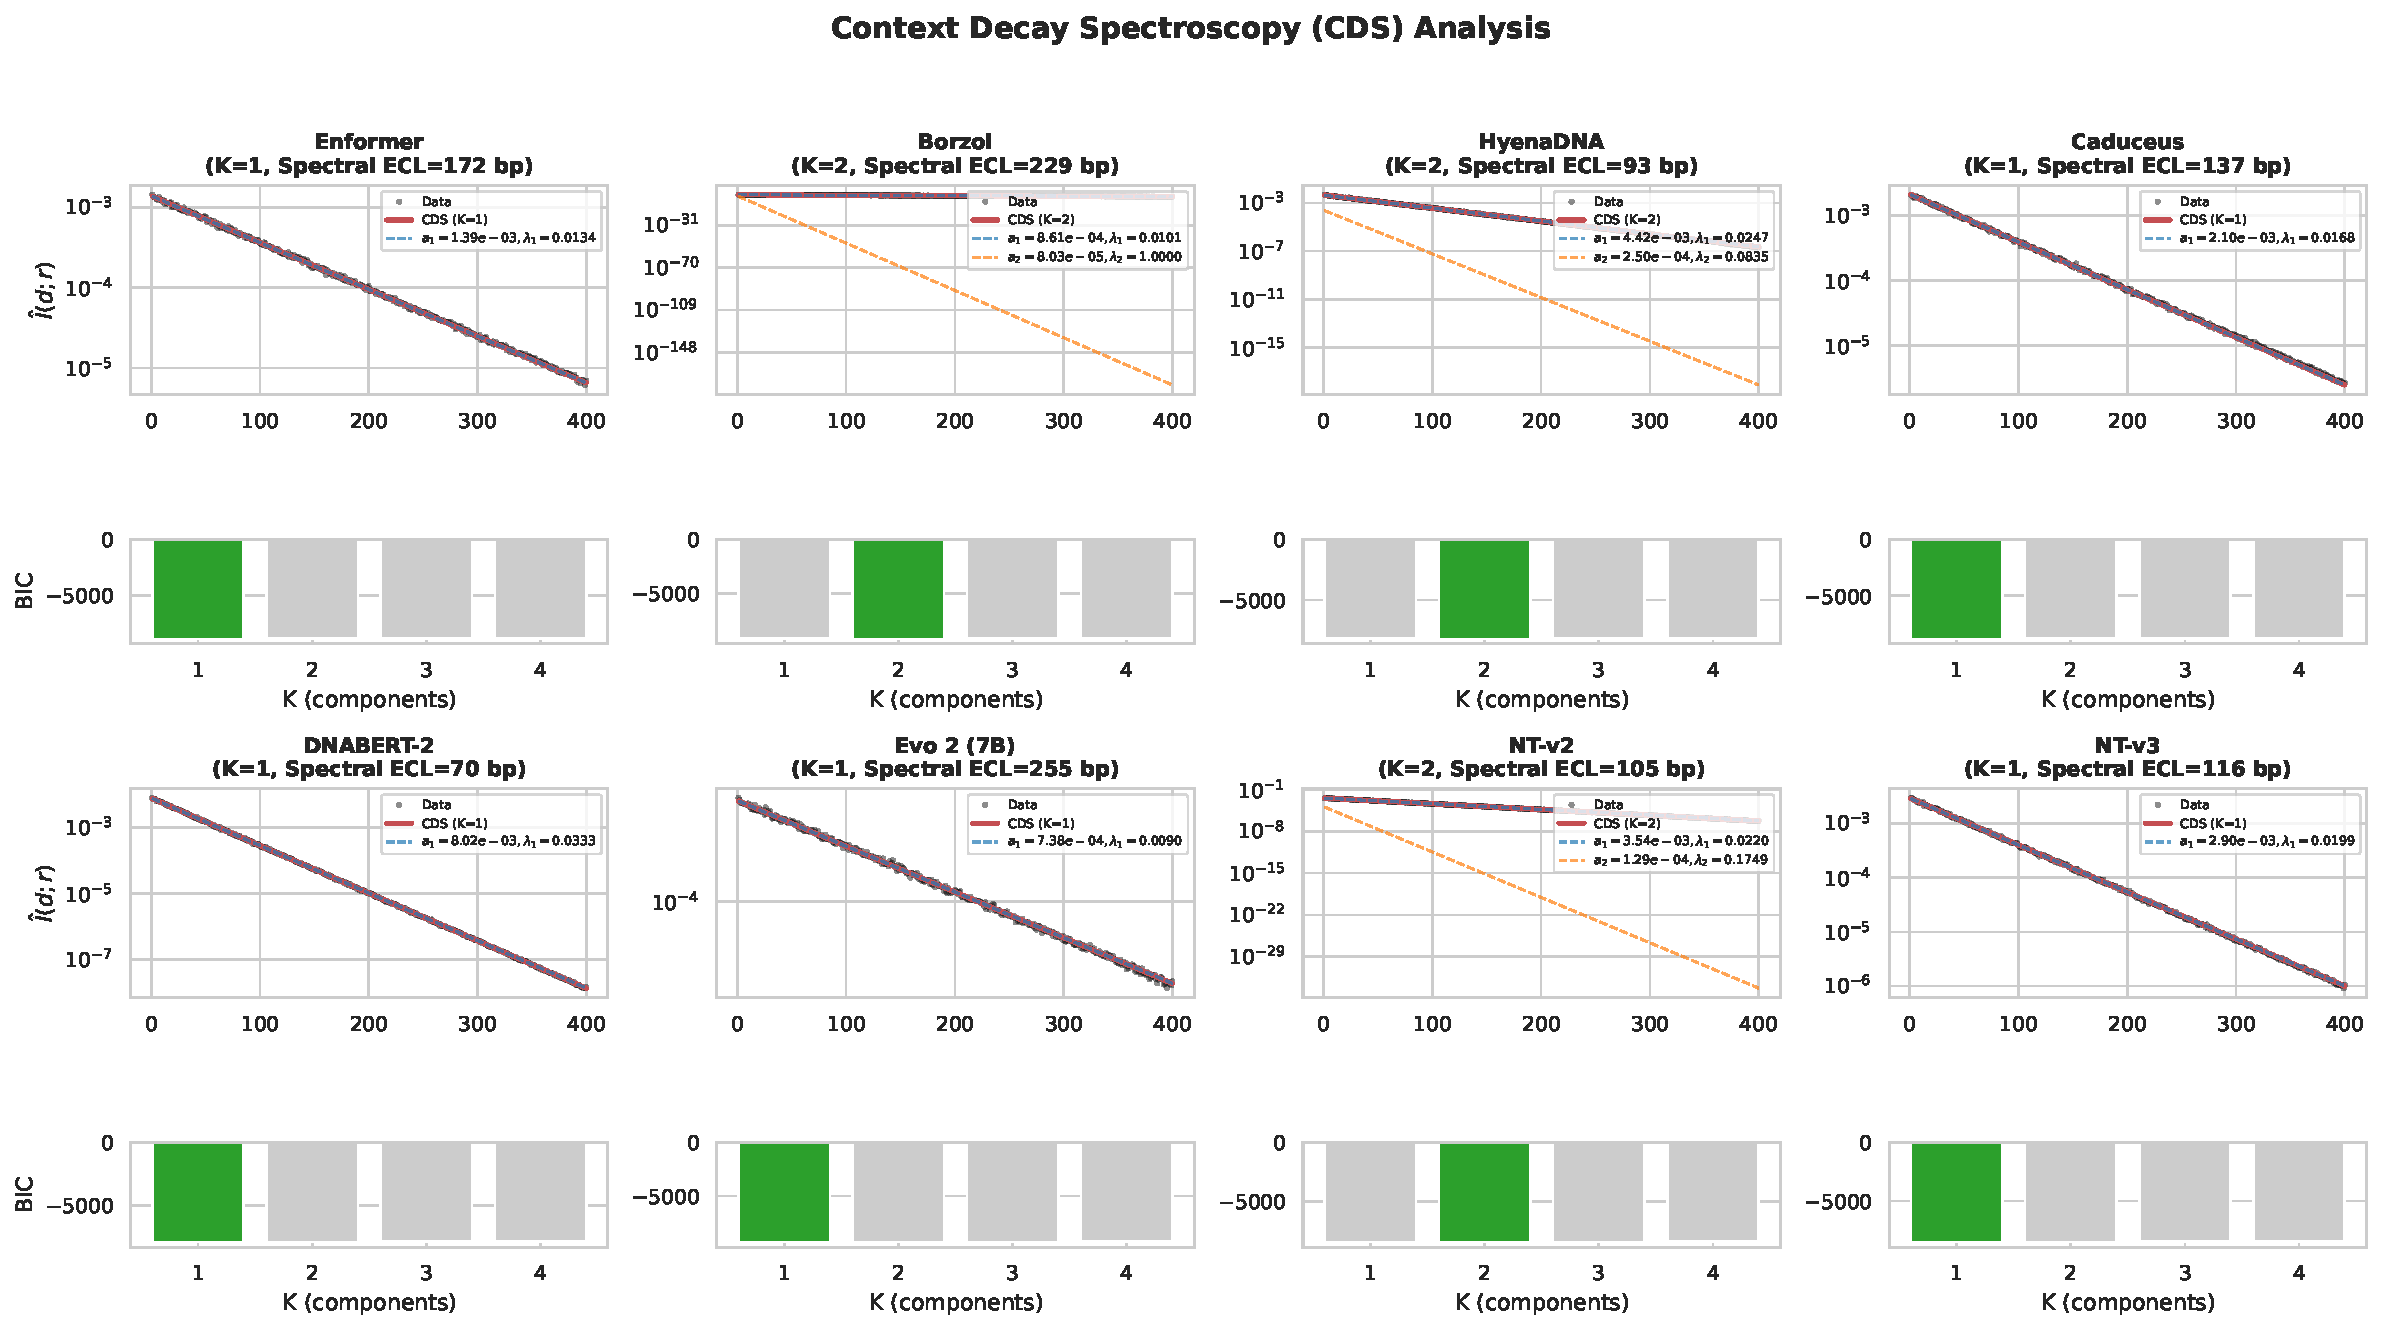
\includegraphics[width=\textwidth]{figures/figA1_cds_analysis.pdf}
\caption{Context Decay Spectroscopy (CDS) analysis for eight models (synthetic surrogates). Top panels: log-scale influence profiles (black dots) with CDS fits (red lines) and individual exponential components (dashed). Bottom panels: BIC model selection over $K \in \{1,2,3,4\}$ components (green = selected). Models with longer decay lengths require fewer components; short-context models exhibit multi-scale decay structure.}
\label{fig:cds_analysis}
\end{figure}

\subsection{ECL vs.\ model performance}

Correlate ECL$_{0.9}$ with downstream task performance (Pearson $r$) across models:
\begin{enumerate}[leftmargin=2em, label=(\roman*)]
\item Gene expression prediction (MSE on held-out genes).
\item Variant effect prediction (Spearman $\rho$ with GTEx eQTL effect sizes).
\item Chromatin accessibility prediction (AUROC on ENCODE peaks).
\end{enumerate}

Expected: models with larger ECL at relevant loci achieve better long-range prediction, but the correlation may be weak if local motif features dominate performance.

\subsection{ECD analysis}

Report Effective Context Dimension distributions across models and locus classes. ECD reveals whether a model distributes influence broadly (high ECD, genuinely using many positions) or concentrates on a few key positions (low ECD).

\begin{figure}[t]
\centering
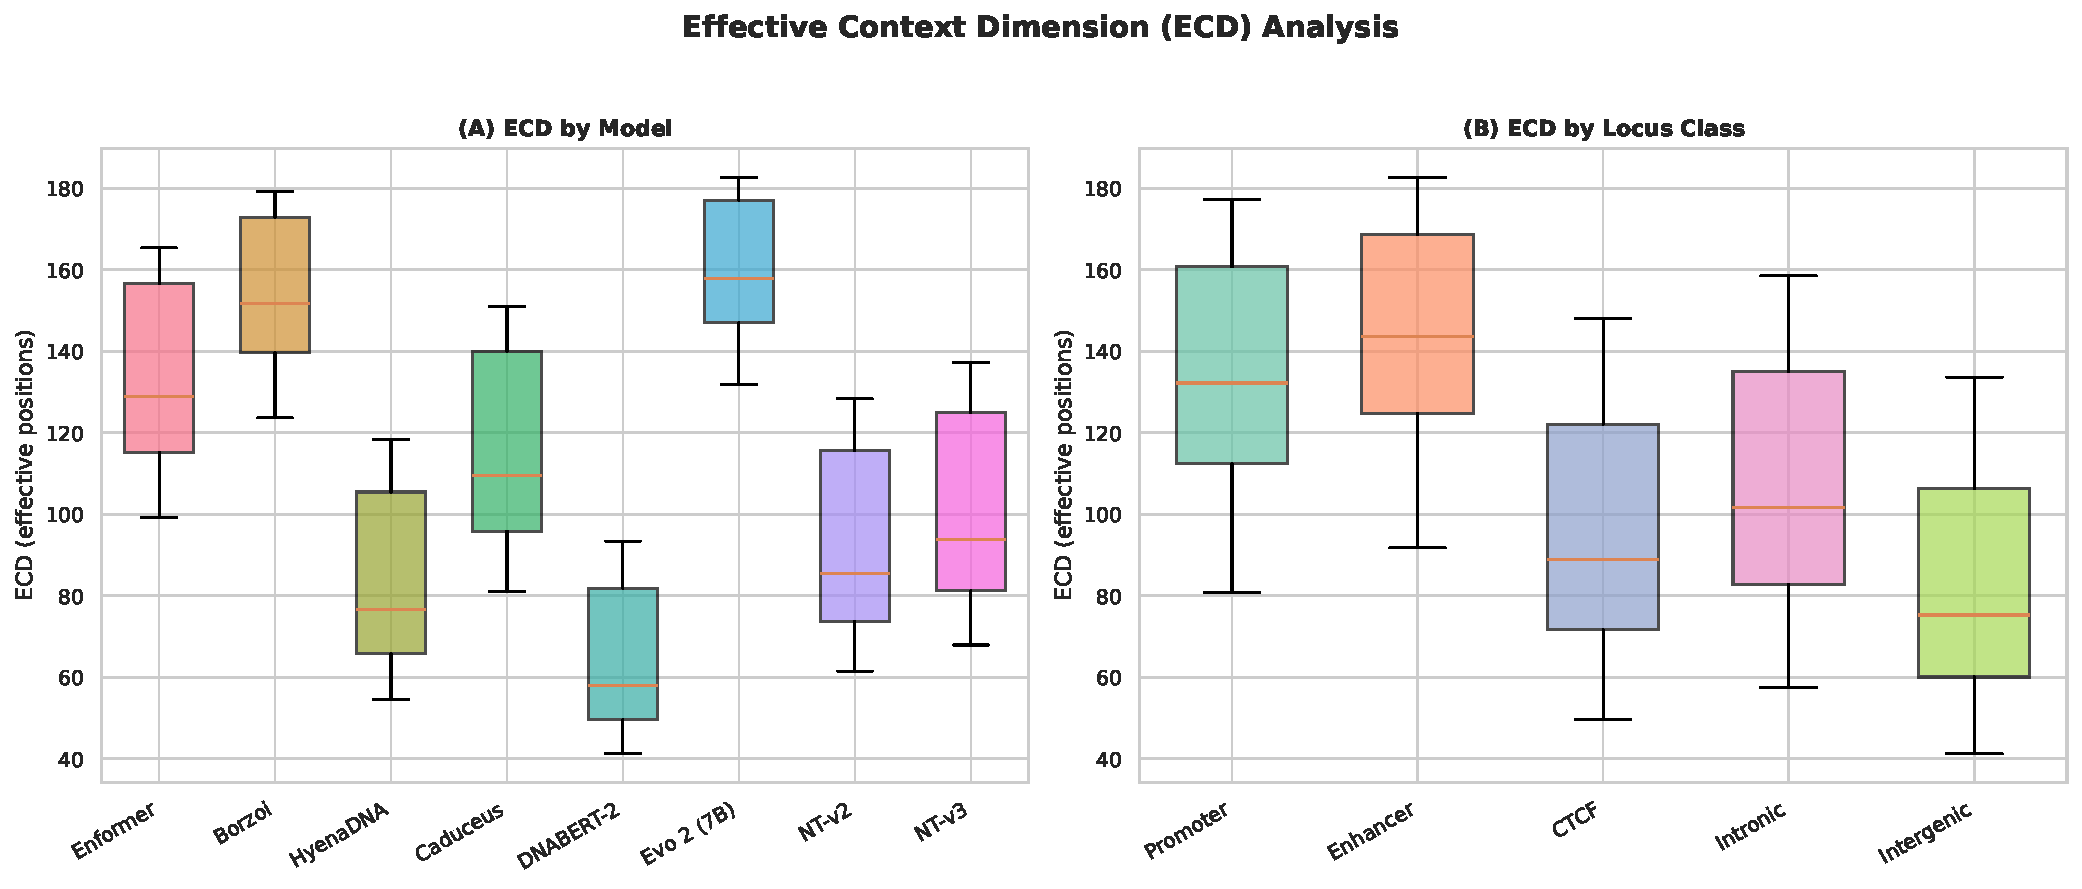
\includegraphics[width=\textwidth]{figures/figA2_ecd_analysis.pdf}
\caption{Effective Context Dimension (ECD) distributions. (A)~ECD by model, aggregated across locus classes. Longer-context models (Evo~2, Borzoi) exhibit higher ECD. (B)~ECD by locus class, aggregated across models. Enhancer and promoter loci show higher ECD than intergenic regions, consistent with their richer regulatory context.}
\label{fig:ecd_analysis}
\end{figure}

\subsection{Positional bias analysis}

Test for ``lost in the middle'' effects in genomic models:
\begin{enumerate}[leftmargin=2em, label=(\roman*)]
\item For Enformer (196~kb window), compute $\cI(i;r)$ for reference positions $r$ at the center, 25\% from edge, and near the edge.
\item Plot influence as a function of absolute position (not distance from $r$).
\item Expected: if positional encoding creates edge bias, influence will be higher for absolute positions near the boundaries regardless of $r$.
\end{enumerate}

% =============================================================================
\section{Implementation Guide}\label{app:implementation}
% =============================================================================

This appendix provides practical guidance for implementing the ECL estimation framework. We describe software architecture, model-specific considerations, and a step-by-step protocol.

\subsection{Software architecture}

We recommend a modular Python implementation with the following components:

\paragraph{Core modules.}
\begin{enumerate}[leftmargin=2em, label=(\roman*)]
\item \texttt{perturbations.py}: Perturbation kernel implementations. Each kernel is a callable: \texttt{perturb(sequence, positions, rng)} $\to$ \texttt{perturbed\_sequence}. Implementations for random substitution, dinucleotide shuffle (using the Altschul--Erickson algorithm), $k$-mer Markov resampling, and generative infilling.
\item \texttt{influence.py}: Influence energy computation. Core function: \texttt{compute\_influence(model, sequences, reference, perturbation, metric, n\_samples)} $\to$ \texttt{influence\_profile}. Supports batched GPU inference.
\item \texttt{ecl.py}: ECL computation from influence profiles. Functions for cumulative influence, ECL at specified $\beta$, ECP, ECD, AECP, directional ECL.
\item \texttt{estimation.py}: Statistical estimation utilities. Bootstrap CI, Bernstein bounds, antithetic estimation, importance sampling, permutation tests.
\item \texttt{cds.py}: Context Decay Spectroscopy. Mixture-of-exponentials fitting via scipy \texttt{curve\_fit} or EM.
\item \texttt{gniah.py}: Genomic Needle-in-a-Haystack protocol.
\end{enumerate}

\paragraph{Model wrappers.}
Each model requires a wrapper class implementing:
\begin{enumerate}[leftmargin=2em, label=(\roman*)]
\item \texttt{forward(sequence)} $\to$ \texttt{embedding}: returns the embedding tensor.
\item \texttt{nominal\_context}: the model's nominal context length in bp.
\item \texttt{token\_to\_bp(token\_idx)} $\to$ \texttt{bp\_position}: position mapping $\phi$.
\item \texttt{embedding\_dim}: dimensionality of the output embedding.
\end{enumerate}

\subsection{Model-specific implementation notes}

\paragraph{Enformer.}
Available via \texttt{enformer-pytorch} or TensorFlow Hub. Input: one-hot encoded DNA of length 196,608 bp. Output: 5,313 tracks at 896 output positions (128 bp resolution). For ECL computation, extract the central bin's embedding vector (or the full 896-position output and analyze per-bin). Use the human head (tracks 0--5,312).

Practical consideration: Enformer's convolutional stem processes 196,608 bp into 1,536 positions before attention. Perturbations at single-nucleotide resolution within a 128~bp bin are largely equivalent due to the initial convolution. Block perturbation at $b=128$ bp is recommended for efficiency.

\paragraph{Borzoi.}
Similar to Enformer but with 524,288 bp input and 32~bp output resolution (16,384 output positions). Uses an ensemble of replicates; average predictions across replicates for stability.

\paragraph{HyenaDNA.}
Available via HuggingFace. Input: character-level DNA tokens. Supports variable context lengths up to 1~Mb. The model produces per-token embeddings; extract the embedding at the reference position $r$. No tokenization mapping needed ($\phi = \mathrm{id}$).

\paragraph{Caduceus.}
BiMamba architecture with reverse-complement equivariance. Input: character-level DNA. The bidirectional architecture means perturbations propagate in both directions, potentially creating different ECL profiles than unidirectional models. Extract embeddings at position $r$ from the final layer.

\paragraph{Evo~2.}
40B parameters; requires multi-GPU inference (at least 4$\times$ A100 80GB). Input: character-level DNA up to 1~Mb. The model is autoregressive (next-token prediction), so the ``embedding'' is the hidden state at position $r$. Note: for autoregressive models, only positions $i < r$ can influence the embedding at $r$ (causal masking), creating an inherent directional asymmetry.

\paragraph{DNABERT-2.}
BPE tokenization with ALiBi positional encoding. Input: tokenized DNA (variable length, $\sim$512 tokens $\approx$ 3~kb). The position mapping $\phi$ is non-trivial due to BPE: each token spans a variable number of base pairs. ECL should be reported in bp using $\phi$.

\subsection{Step-by-step protocol}

\paragraph{Step 1: Locus selection.}
\begin{enumerate}[leftmargin=2em, label=(1.\arabic*)]
\item Download GENCODE annotations (v44) and ENCODE cCRE annotations.
\item Select 500 promoter-centered loci (TSS $\pm$ half of nominal context), 500 enhancer-centered loci (distal cCREs $>$10~kb from nearest TSS), 500 random intronic controls.
\item Exclude loci on training chromosomes; use chr8 and chr9 (held-out for Enformer/Borzoi).
\item Extract reference genome sequences (hg38) centered on each locus.
\end{enumerate}

\paragraph{Step 2: Perturbation generation.}
\begin{enumerate}[leftmargin=2em, label=(2.\arabic*)]
\item For each sequence and each distance bin $d \in \{0, 1, 2, 5, 10, 20, 50, 100, 200, 500\}$ kb:
\item Sample $m(d) = 10$ positions at distance $d$ from the reference, increasing $m(d)$ near the threshold-crossing distance per \cref{alg:adaptive} (adaptive sampling) when a coarse pilot already locates the threshold.
\item Generate perturbed sequences under each perturbation type.
\item Cache perturbed sequences to avoid regeneration during bootstrap.
\end{enumerate}

\paragraph{Step 3: Forward pass computation.}
\begin{enumerate}[leftmargin=2em, label=(3.\arabic*)]
\item For each sequence: compute the reference embedding $f(X)$.
\item For each perturbation: compute $f(X^{(i)})$.
\item Compute $d_\cZ(f(X), f(X^{(i)}))$ for each perturbation.
\item Store all pairwise distances for bootstrap resampling.
\end{enumerate}

\paragraph{Step 4: Influence profile and ECL computation.}
\begin{enumerate}[leftmargin=2em, label=(4.\arabic*)]
\item Average pairwise distances within each distance bin.
\item Compute cumulative influence and normalize.
\item Find ECL$_\beta$ for $\beta \in \{0.5, 0.8, 0.9, 0.95, 0.99\}$.
\item Compute ECP, ECD, AECP, directional ECL.
\end{enumerate}

\paragraph{Step 5: Uncertainty quantification.}
\begin{enumerate}[leftmargin=2em, label=(5.\arabic*)]
\item Run $B=1{,}000$ bootstrap resamples.
\item Report percentile CIs for all quantities.
\item Compute Bernstein-based analytical CIs for comparison.
\end{enumerate}

\paragraph{Step 6: Visualization and reporting.}
\begin{enumerate}[leftmargin=2em, label=(6.\arabic*)]
\item Generate all proposed figures and tables.
\item Run hyperparameter sensitivity checks (\cref{app:sensitivity}).
\item Compare across models using the permutation test.
\end{enumerate}

\subsection{Recommended hardware}

\begin{table}[H]
\centering
\caption{Hardware requirements per model for a complete ECL analysis (500 loci, binned estimator).}
\label{tab:hardware}
\small
\begin{tabular}{@{}l l l l@{}}
\toprule
\textbf{Model} & \textbf{GPU memory} & \textbf{Estimated time} & \textbf{GPU type} \\
\midrule
Enformer & 16 GB & $\sim$14 hours & 1$\times$ A100 \\
Borzoi & 32 GB & $\sim$28 hours & 1$\times$ A100 80GB \\
HyenaDNA & 16 GB & $\sim$8 hours & 1$\times$ A100 \\
Caduceus & 8 GB & $\sim$4 hours & 1$\times$ A100 \\
Evo~2 & 320 GB & $\sim$12 days & 4$\times$ A100 80GB \\
DNABERT-2 & 8 GB & $\sim$2 hours & 1$\times$ A100 \\
\bottomrule
\end{tabular}
\end{table}

\subsection{Numerical considerations}

\begin{enumerate}[leftmargin=2em, label=(\roman*)]
\item \textbf{Numerical precision:} Use float32 for embeddings; float64 for cumulative sums and ECL computation to avoid rounding errors in threshold comparisons.
\item \textbf{Embedding normalization:} For models with very high-dimensional embeddings ($d > 3{,}000$), normalize embeddings to unit norm before computing distances to avoid numerical overflow. Report whether normalization was applied.
\item \textbf{Zero-influence positions:} Positions with $\widehat{\cI}(i;r) < \varepsilon_{\mathrm{machine}}$ should be treated as zero. This affects ECD computation (entropy with near-zero probabilities).
\item \textbf{Boundary handling:} Positions within $R_{\mathrm{boundary}}$ bp of sequence edges should be excluded or flagged, as boundary effects can inflate apparent ECL.
\end{enumerate}

% =============================================================================
\section{Annotated Reference Guide}\label{app:references}
% =============================================================================

This appendix provides annotated summaries of key references organized by topic, intended as a guide for readers entering the field.

\subsection{Genomic sequence models}

\paragraph{\citet{Avsec2021Enformer}: Enformer.}
Introduced transformer attention for gene expression prediction from 196~kb DNA input. Key contribution: demonstrated that attention-based long-range interactions improve over pure CNNs (Basenji2). The paper's ``contribution scores'' analysis showed that attention enables the model to integrate enhancer signals at $>$20~kb, but most predictive signal remains promoter-proximal. Directly motivates ECL measurement.

\paragraph{\citet{Linder2025Borzoi}: Borzoi.}
Extended Enformer to 524~kb with RNA-seq coverage prediction at 32~bp resolution. Predicts 7,611 tracks across human and mouse. Key insight: longer context improves splicing and isoform-level predictions. The 32~bp output resolution makes block perturbation at $b=32$ natural.

\paragraph{\citet{Nguyen2023HyenaDNA}: HyenaDNA.}
First genomic model at 1~Mb single-nucleotide resolution using the Hyena implicit convolution operator. Demonstrated that perplexity improves with context length up to 1~Mb. Small parameter count ($<$7M) raises questions about how much long-range information is captured in practice.

\paragraph{\citet{Schiff2024Caduceus}: Caduceus.}
Bidirectional Mamba (BiMamba) with reverse-complement equivariance. The authors report achieving competitive performance with 10$\times$ fewer parameters than transformer baselines on variant effect prediction. The bidirectional architecture is significant for ECL: both upstream and downstream context can influence each position, unlike autoregressive models.

\paragraph{\citet{Brixi2025Evo2}: Evo~2.}
The authors report a 40B-parameter StripedHyena-Transformer hybrid processing 1~Mb inputs, trained on 9.3~trillion base pairs across all domains of life. Currently the largest reported genomic language model. The hybrid architecture (predominantly SSM with sparse attention) creates a distinctive ECL profile that may differ from pure transformers or pure SSMs.

\paragraph{\citet{Benegas2026AlphaGenome}: AlphaGenome.}
Google DeepMind's 1~Mb supervised model predicting thousands of genomic tracks. Notably acknowledges that predictions degrade for genes $>$100~kb from the input center, providing an informal ECL estimate of $\sim$100~kb.

\subsection{Context utilization in NLP}

\paragraph{\citet{Liu2024LostInMiddle}: Lost in the Middle.}
Demonstrated the U-shaped retrieval accuracy curve in LLMs: information at the beginning and end of context is well-used; middle positions are underweighted. The genomic analogue would be positional bias in Enformer/Borzoi attention.

\paragraph{\citet{Hsieh2024RULER}: RULER.}
Benchmark defining effective context as the maximum length maintaining $>$85.6\% performance across 13 tasks. Found most open-source models use $<$50\% of claimed context. RULER's operational definition is task-specific; our perturbation-variance ECL complements it with a task-agnostic, embedding-level measure.

\paragraph{\citet{An2024EffCtx}: Why ECL Falls Short.}
Identified left-skewed position frequency distributions during pretraining as the root cause of short ECL. Their STRING method shifts well-trained positions to overwrite undertrained ones, improving long-context performance without retraining.

\subsection{Sensitivity analysis and attribution}

\paragraph{\citet{Saltelli2010VarianceSA}: Variance-based sensitivity analysis.}
The foundational reference for Sobol indices and total-effect indices. Provides the mathematical framework for decomposing output variance into input contributions. Our connection between perturbation influence and Sobol indices (\cref{thm:sobol_equiv}) builds directly on this work.

\paragraph{\citet{Fel2021Sobol}: Sobol attribution for neural networks.}
Applied Sobol-based sensitivity analysis to explain neural network predictions using perturbation masks from quasi-Monte Carlo sequences. Demonstrated efficiency over standard perturbation methods. Directly relevant to our surrogate-accelerated ECL (\cref{alg:surrogate}).

\paragraph{\citet{Toneyan2024CREME}: CREME.}
Toolkit for measuring context dependence in genomic models via dinucleotide shuffling of distal regions. Found that Enformer's expression predictions are largely insensitive to distal sequence, while some silencer effects extend over the full receptive field. CREME's methodology is a special case of our out-of-window ablation $\Delta_{\mathrm{out}}$.

\paragraph{\citet{Karollus2023Limited}: Enformer's limited distal sensitivity.}
Showed via progressive masking that Enformer captures regulatory determinants mainly in promoters, and that predicted variant effects decay rapidly with distance, unlike experimentally measured effect sizes. This is precisely the nominal--effective gap that ECL formalizes.

\subsection{Information theory and decision theory}

\paragraph{\citet{Blackwell1951Comparison}: Comparison of experiments.}
Foundational paper establishing that one information source (experiment) is more informative than another if and only if it achieves lower Bayes risk for all decision problems. We apply this to compare context-limited embeddings across models (\cref{sec:blackwell}).

\paragraph{\citet{Barbero2024OverSquashing}: Over-squashing in transformers.}
Established theoretical bounds on information propagation in decoder-only transformers, showing that sensitivity to distant tokens depends on the sum of weighted paths through the attention graph. Implies that even with unlimited nominal context, architectural bottlenecks limit effective context.

\subsection{SSMs and architectural alternatives}

\paragraph{\citet{Gu2023Mamba}: Mamba.}
Introduced selective state-space models with input-dependent gating, achieving linear-time sequence modeling. The selective mechanism allows the model to dynamically choose what to remember, creating position-dependent context utilization patterns.

\paragraph{\citet{Dao2024Mamba2}: Mamba-2 and SSD.}
Established the Structured State Space Duality, proving mathematical equivalence between SSMs and linear attention. This theoretical unification explains why hybrid SSM-attention architectures (StripedHyena, Evo) work well: SSMs provide efficient long-range context compression, while sparse attention provides selective precise recall.

\paragraph{\citet{Jelassi2024Copying}: Copying limitations of SSMs.}
Proved that any model with fixed-size memory is fundamentally limited at copying long random strings. For genomics, this implies that SSM-based models may fail to propagate precise sequence information (e.g., exact motif sequences) over very long distances, even if they capture statistical patterns.

\subsection{Causal interpretability}

\paragraph{\citet{Kendiukhov2026MechInterp}: Mechanistic interpretability critique.}
Showed that attention-based gene regulatory network extraction fails in single-cell models, with trivial baselines outperforming attention-derived networks. Demonstrates that observational measures (attention maps) are unreliable indicators of functional context utilization, motivating interventional approaches like our perturbation-based ECL.

\paragraph{\citet{Goodfire2025Evo2}: SAEs on Evo~2.}
Trained sparse autoencoders on Evo~2 representations, recovering biologically interpretable features (coding regions, TFBS, tRNA, exon-intron boundaries). Suggests that genomic models learn rich internal representations, but does not address whether these representations are causally driven by long-range context.


\end{document}
